\documentclass[oneside,10pt]{memoir}
\usepackage{OFP}
\usepackage{tikz}

\makeindex

\begin{document}

\newcommand{\titlefont}{\color{red!30!black}\bfseries}

\begin{flushright}
\thispagestyle{empty}

\vspace{1cm}
\Large
\textbf{Самойленко~С.\,Б.}\\
\textbf{Хан~П.\,В.}
\normalfont

\vspace{2cm}

\hrule
\bigskip
           \HUGE\titlefont
            Функциональное\\
            программирование\\
            \huge\normalcolor\normalfont
            в примерах и задачах
\bigskip
\hrule
\vspace{2cm}
% \begin{SchemeCode}[emph={n,b,f,x},
% basicstyle={\schemestyle\color{gray!80!blue}},
% classoffset=0,
% keywordstyle={\schemestyle\color{gray!80!purple}},
% classoffset=1,
% keywordstyle={\bfseries\color{gray!70!blue}},
% classoffset=0,
% emphstyle={\itshape\color{gray!80!blue}}]
%     (define fact (Y Ф))
    
%     (define Y (lambda(b) ((lambda(f) (b (lambda(x) ((f f) x))))
%                      (lambda(f) (b (lambda(x) ((f f) x)))))))
%     (define Ф
%       (lambda(f)
%         (lambda(n)
%           (if (zero? n) 
%               1 
%               (* n (f (- n 1)))))))

% \end{SchemeCode}
\vfill
\normalsize
Петропавловск-Камчатский\\
2012 г.

\end{flushright}


% %!TEX root = main.tex
% revision is done
\Chapterr{Предисловие}
\small

Это пособие создавалось, как помощь студентам для проведения лабораторных работ по курсу «Функциональное и логическое программирование». Оно содержит минимум теоретического материала и, в основном, освещает практические вопросы, возникающие при изучении курса. 

Учебники по функциональному программированию условно можно разделить на две группы: одни используют для примеров языки семейства \Lang{ML} (\Lang{OCaml}, \Lang{Hope}, \Lang{Haskell} и т.д.), другие основываются на семействе \Lang{Lisp} (чаще всего, \Lang{Common Lisp} или \Lang{Scheme}), несмотря на то, что \Lang{Lisp} не является чисто функциональным. Мы пошли по второму пути: для всех иллюстраций и примеров используется язык \Scheme~--- диалект языка \Racket, разработанный специально для этого курса. В свою очередь \Racket является потомком замечательного языка \Lang{Scheme}.

Язык \Lang{Racket} был выбран по следующим причинам. Минимальность основных средств этого языка и его гибкость позволяют сосредоточиться на алгоритмах и принципах функционального программирования, практически не отвлекаясь на изучение самого языка. Расширяемость \Racket позволяет с помощью одних только базовых средств построить многие специфические для функционального программирования конструкции, такие как ленивые потоки, монады, абстрактные алгебраические типы, продолжения и т.\,п. Рассмотрение и построение этих концепций <<с нуля>> позволяет глубже понять их принципы и грамотно применять их в <<серьёзных>> языках, таких как \Lang{Haskell} или \Lang{Erlang}.
Сам \Lang{Racket} является полноценным, активно развивающимся языком программиррования общего назначения, предназначенным для быстрого прототипирования, разработки новых экспериментальных концепций теоретического программирования, создания веб-серверов и приложений и т.д. Он обладает очень богатым инструментарием и замечательно документирован. Кроме того, для этого языка существует удобная свободно распространяемая интегрированная среда разработки \Lang{DrRacket}. Не последнюю роль сыграло и то, что именно \Lang{Scheme} используется в замечательных фундаментальных учебниках по общему программированию: <<Структура и интерпретация компьютерных программ>>, Х. Абельсон и др. или <<Как разрабатывать программы>>, М. Феллайзен и др. 

Мы намеренно используем только очень незначительную часть инструментария, предоставляемого языком \Racket. К примеру, мы не будем рассматривать разнообразные специфические типы данных, которые представлены в языке: структуры, векторы, объекты и пр., не будем пользоваться ключами при определении и использовании функций, ограничимся написанием только самых примитивных макросов. Кроме базовых функций и форм языка, мы воспользуемся подстановками с механизмом сопоставления с образцом и бесточечной нотацией, которые позволят нам писать более прозрачный код и помогут читателю освоить такие языки, как \Lang{OCaml}, \Lang{Haskell}, \Lang{Prolog}, \Lang{Mathematica}~и~т.\,п.
 
Мы не собираемся учить языку \Racket или \Lang{Scheme}; наша задача~--- дать практические навыки функционального программирования, по существу, в отрыве от какого-либо конкретного языка. И как раз для этой задачи \Racket подходит замечательно. Все главы, в которых вводятся новые понятия и концепции функционального программирования, имеют раздел, в котором указывается, в каких ещё распространённых языках программирования можно ими пользоваться.

Книга предназначена, в первую очередь, для студентов информационно\-/технических специальностей, как учебное пособие. Но она будет полезна для преподавателей, в качестве дидактического материала, а так же для всех, интересующихся программированием и желающих получить представление о функциональном программировании.

\tableofcontents*

\renewcommand\listtablename{Указатель заданий}

\listoftables*
\normalsize
  % %!TEX root = main.tex
% revision is done
\Chapter{Введение}

\section{Парадигмы программирования}%
Когда-то, не~очень давно, работа программиста называлась «кодированием», а~программа~--- «машинным кодом». В~самих этих названиях есть что-то от~шпионских игр и~шифровки. Программисты переводили метод решения прикладных задач на~язык алгоритмов, понятный человеку, а~алгоритмы~--- в~последовательность инструкций, понятных машине. Таким образом, программа воспринималась, как текст, предназначенный для машины, а~не для человека. Для того, чтобы человек мог разобраться в~этих инструкциях, для их отладки или модификации, разрабатывались те или иные \emph{парадигмы программирования}~--- стилистические и~методологические концепции, позволяющие приблизить процесс написания и~чтения программы к~человеческому восприятию и~к предметной области решаемых программистом задач.

Разделяют две противоположные парадигмы программирования: \index{парадигма программирования!императивная}\emph{императивную} и~\index{парадигма программирования!декларативная}\emph{декларативную}. Само слово «программа» подразумевает некоторую последовательность действий, предписанную для выполнения задачи. В~этом и~проявляется императивный подход. В~нём программой является последовательность инструкций, а~вычислительным процессом~--- последовательность состояний вычислительной среды. При~декларативном подходе программа превращается в~совокупность набора определений, описывающих условие решаемой задачи, и~набора соотношений, показывающих, в~чём состоит её решение.

\index{парадигма программирования!функциональная}\emph{Функциональное программирование} (ФП)~--- это одна из~парадигм декларативного программирования. В~ней описание процесса решения задачи сводится к~определению набора функций, а~постановку задачи определяют аргументы, передаваемые этим \mbox{функциям}.

В математике \index{функция}\emph{функция}~--- это отображение из~области определения в~область значений. Когда мы говорим о~функции $f(x)$, мы одновременно подразумеваем и~процедуру отображения и~результат этого отображения: в~определённом смысле, мы в~праве смешивать эти два понятия. Такой подход к~функциям оказался пригодным и~очень продуктивным для программирования. Когда мы представляем программу, как набор функций, мы можем воспринимать их, в~зависимости от~необходимости, как процессы или как результаты, то есть, как данные.

Перечислим основные принципы ФП:

\begin{enumerate}
 \item Программирование не~опирается на~хранение состояния вычислительной среды. Вместо этого вычисляются результаты чистых функций от~исходных данных и~результатов других функций.

 \item Использование функций, как \emph{объектов первого класса}. Это значит, что функции можно использовать как данные: создавать их во~время выполнения программы, передавать их в~качестве аргументов другим функциям и возвращать в качестве результатов.

 \item Из~предыдущего вытекает возможность писать и~использовать функции высших порядков и~функционалы~--- функции, аргументами и~значениями которых являются другие функции.

 \item Использование \emph{чистых функций}~--- функций не~имеющих побочных эффектов, зависящих только от~своих аргументов и~только возвращающих свой результат.

 \item Применение \emph{рекурсии}, как основного способа описания циклических процессов.

 \item \emph{Интенсивные} и~\emph{ленивые} \emph{вычисления}, различающиеся порядком, в~котором обрабатываются аргументы функций.

\end{enumerate}

Самое же главное --- разработанная в~математике строгая теория функций применима и~к функциональным программам. Из~перечисленных нами особенностей вытекают следующие достоинства~ФП:

\begin{enumerate}
 \item Возможность строгого доказательства корректности программы и, как следствие, повышение надёжности кода.

 \item Возможность существенной оптимизации программы при~компиляции.

 \item Высокая степень абстракции и~связанные с~этим удобочитаемость, расширяемость и~переносимость программ.

 \item Использование чистых функций существенно повышает модульность программ и~упрощает организацию параллельных вычислений.
\end{enumerate}

При изучении данного курса следует помнить, что достоинства функционального программирования не~определяются достоинствами того или иного языка программирования, \Lang{Scheme} или \Lang{Haskell}, например. Они относятся к~функциональному подходу в~целом, как к~модели вычислений и~модели построения программ и~структур данных. Эта модель возникла раньше модели Тьюринга и~частично легла в~её основу. Если сначала функциональное программирование носило, преимущественно, теоретический характер, как важный инструмент теории вычислений и~алгоритмов, а~потом долго не~выходило за~рамки специализированных функциональных языков программирования, то сейчас функциональный инструментарий включается во~многие широко используемые на~практике языки: \Lang{C\#}, \Lang{Python}, \Lang{Perl}, \Lang{JavaScript} и~т.\,д. Кроме того, и~существенно функциональные языки, такие, как \Lang{OCaml}, \Lisp, \Lang{Erlang,} \Lang{Haskell}, \Lang{F\#} давно вышли из~академической среды и~стали использоваться для решения самых разных практических и~промышленных задач.

\section[4]{Зачем изучать функциональное программирование?}%
Освоение функциональной парадигмы прививает определённый стиль программирования, имеющий универсальные достоинства~--- писать «функционально» можно практически на~любом высокоуровневом языке программирования. При~этом программы становится легче читать, отлаживать и~расширять. Меняется и~подход к~формулировке задач: она становится более строгой и~предметно-ориентированной.{\tolerance=800\par}

Кроме того, большинство современных промышленных языков программирования имеет функциональный инструментарий, и~квалифицированный специалист должен уметь использовать его в~полной мере.

Наконец, немаловажным оказывается и~субъективное восприятие той или иной парадигмы. При~императивном подходе программист является «диктатором»~--- машина, получая от~него список непреложных указаний, находится в~подчинённом положении. Процесс декларативного программирования можно воспринимать, как обучение машины человеком, как передачу знаний и~умений, зачастую, превращающееся в~совместное с~машиной исследование предметной области. Именно функциональные языки программирования используются для разработки искусственного интеллекта, экспертных систем, систем обработки символьных и~вербальных данных.

\section[2]{Язык Formica}%
Для примеров в этой книге используется язык \FLP{}\footnote{https://github.com/samsergey/formica} --- диалект языка \Scheme. В свою очередь, \Scheme является наследником замечательного языка \Lang{Scheme}.

\Lang{Scheme}~--- это \emph{язык программирования высокого уровня}, один из~двух наиболее популярных в~наши дни диалектов языка \Lisp. Язык \Lang{Scheme} был создан в~середине 1970-х годов и~с тех пор широко используется и~развивается. Он, наряду с~\Lisp-ом, используется, для написания скриптов и~сценариев, например, в~таких программах, как \Lang{AutoCAD}, \Lang{Gimp}, \Lang{Emacs} и~пр. Кроме того, эти языки используются для оптимизации трансляторов и~компиляторов, для синтаксического разбора текстов; на~них пишут серверы и~веб-приложения, экспертные системы и~системы компьютерной алгебры, а~так~же многие другие приложения. Существует множество интерпретаторов и~компиляторов \Lang{Scheme}, как свободных, так и~проприетарных.

Разработчики \Lang{Scheme} старались не~нарушить элегантность и~простоту языка, его подчёркнуто минималистскую философию. Цель создания \Lang{Scheme}~--- не~собирать воедино разные полезные конструкции и~средства, а~удалить слабости и~ограничения, вызывающие необходимость добавления в~язык новых возможностей. В~результате, язык содержит минимум примитивных конструкций и~позволяет выразить всё что угодно, путём надстройки над~ними. Девиз языков семейства \Lisp: «\Lisp~--- программируемый язык программирования». По~существу, программирование на~\Lang{Scheme}~--- это создание новых языков, заточенных под~решаемые задачи.

Язык \Lang{Scheme} и его диалекты могут быть полезны в~повседневной работе программиста, даже если он использует для работы совсем другие языки. С~их помощью можно детально разрабатывать алгоритмы, концентрируясь на~существе разрабатываемого вычислительного процесса, на~вопросах корректности и~эффективности алгоритма, не~отвлекаясь, до~поры до~времени, на~детали ввода-вывода или на~менеджмент памяти.

\Lang{Scheme} не~является чистым функциональным языком, как, например, \Lang{Haskell}, но принципы, лежащие в~его основе, дают возможность писать чисто функциональные программы. Более того, этот язык позволит нам самостоятельно разработать практически весь необходимый инструментарий для полноценного программирования в~рамках функциональной парадигмы.

\subsection{Особенности Formica}%
Перечислим основные особенности \FLP:

\begin{itemize}
  \item Упрощённый синтаксис для каррирования и частичного применения функций.
  \item Наличие подстановок, реализующих технику переписывания и сопоставления с образцом.
  \item Наличие формальных функций, служащих для отладки функциональных программ, 
  а так же для определения абстрактных и алгебраических типов данных.
  \item Встроенные средства для мемоизации функций.
  \item Инструментарий для определения и использования монад.
\end{itemize}

\section{Обозначения, принятые в~тексте}%
Приводя код на~языке \Scheme, мы будем выделять с~помощью различных шрифтов различные объекты:

\begin{itemize}[\ ]
  \item \s{cons list sin} ...~--- базовые функции; 
  \item \s{define let if} ...~--- специальные формы;
  \item \s{fold f sum} ...~--- определяемые нами функции;
  \item \lex{x y expr} ...~--- формальные аргументы функций;
  \item \s[emph={}]{1 2.3 #t "abc"} ...~--- константы;
  \item \s{; some text}~--- комментарии.
\end{itemize}

\section[2]{Программа DrRacket}%
Программа \Lang{DrRacket}\footnote{http://racket-lang.org/.} является интегрированной средой разработки программ для диалектов языка \Lang{Scheme}. Она включает в~себя редактор, компилятор и~интерпретатор, отладчик, менеджер программных модулей и~другие инструменты. Кроме этого, в~дистрибутив входит полная документация по~языку \Racket (на английском языке) и русскоязычная документация по \Scheme, которая находится в разделе \textbf{Getting started} (меню \MenuItem{Help | Help Desk}).

Программа разработана в~рамках проекта PLT (Programming Language Teaching) и~является свободно распространяемым продуктом. Существуют реализации программы \Lang{DrRacket} для различных платформ: MS Windows, Linux, MacOS и~др. Данный курс опирается на~версию \Lang{DrRacket} 5.3.1 или повышение.

Приведём основные команды программы \Lang{DrRacket}, которые нам потребуются:

\medskip
\noindent
\begin{threeparttable}
\begin{tabular}{p{0.35\textwidth}p{0.15\textwidth}>{\comment\baselineskip=9pt}p{0.4\textwidth}}\toprule
\bfseries Меню & \bfseries Клавиатура & \normalfont\bfseries Описание\\\midrule
-- & \MenuItem{F1} &
Вызывает контекстную справку по~функциям \Scheme и \Racket.\\

\MenuItem{Help | Help Desk} & -- &
Открывает браузер с~документацией.\\

\MenuItem{View | Hide Definitions} & \MenuItem{Сtrl\,+\,D}&
Скрывает окно определений, оставляя окно интерпретатора.\\

\MenuItem{View | Hide} \MenuItem{Interactions} & \MenuItem{Сtrl\,+\,E} &
Скрывает окно интерпретатора, оставляя окно определений.\\

\MenuItem{Racket | Run} & \MenuItem{F5} или\MenuItem{} 
\MenuItem{Ctrl\,+\,T} &
Интерпретирует определения и~выполняет программу.\\

\MenuItem{Racket | Ask the program to Quit} & \MenuItem{Ctrl\,+\,B} &
Прерывает выполнение программы.\\

-- & \MenuItem{F6} &
Показывает синтаксическую структуру программы.\\

\MenuItem{Racket | Reindent All} & \MenuItem{Ctrl\,+\,I} &
Выполняет автоматическое выравнивание выражений.\\

-- & \MenuItem{Alt\,+\,P},  \MenuItem{Alt\,+\,N} &
Выполняют навигацию по~ранее введённым командам интерпретатора: \MenuItem{Alt\,+\,P}~--- предыдущая, \MenuItem{Alt\,+\,N}~--- следующая.\\\bottomrule
\end{tabular}
\end{threeparttable}
\medskip

\section{Цикл интерпретатора}%
Как и~многие функциональные языки программирования, \Scheme может работать в~режиме интерпретатора. Это позволяет быстро отлаживать небольшие части кода, отдельные функции и,~таким образом, упрощает процесс разработки \mbox{программы}.

Окно \Lang{DrRacket} обычно разделено на~две части: окно определений (программ) и~окно диалога с~интерпретатором (см. иллюстрацию).
\vspace{-\medskipamount}
\begin{center}
\begin{tikzpicture}
   \node at (0,0) {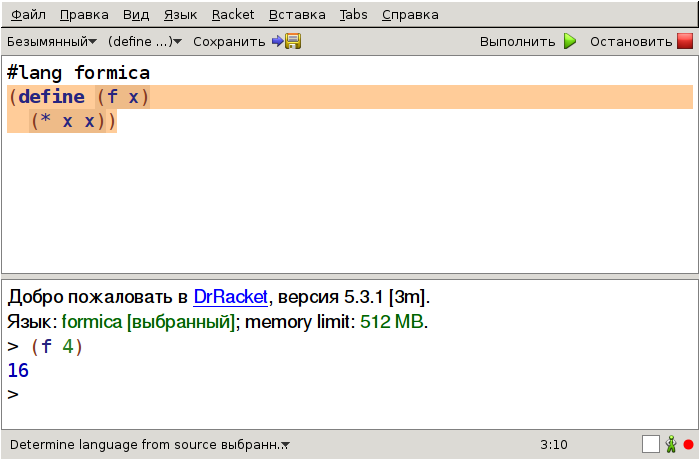
\includegraphics[width=0.9\textwidth]{../figures/DrRacket.png}}; 
   \node at (0,1) {\textsl{область определений}};
   \node at (0,-2) {\textsl{область диалога}};
   \end{tikzpicture}
\end{center}

В нижней части окна программы \Lang{DrRacket} находится окно диалога с~интерпретатором. Приглашение к~вводу выглядит, как «> ». После того, как введено выражение, оно вычисляется при~нажатии клавиши \MenuItem{Enter}, при~этом курсор должен находиться в~конце вычисляемого выражения, в~противном случае, будет просто введён символ разрыва строки.

\begin{example}{%
Введём константу и~нажмём клавишу \MenuItem{Enter}. Интерпретатор вернёт результат.}

\REPL
  {5}
  {5}

\end{example}

\section{Как читать эту книжку?}%
Замечательной особенностью языков\=/интерпретаторов является возможность создавать очень короткие программы\=/вопросы и~программы\=/эксперименты, а~так же получать незамедлительный ответ интерпретатора. Это делает процесс обучения активным и~увлекательным.

Все разделы нашей книги сопровождаются большим числом примеров; каждый из~них может быть выполнен в~программе \Lang{DrRacket}. Участки кода, которые можно использовать в~качестве программ выделены в~тексте следующим образом:

\begin{Definition}
(define func
 ...)
\end{Definition}

Некоторые примеры представлены в~виде короткого диалога с~интерпретатором:

\REPL
  {(question ...)}
  {answer}

Все эти примеры мы рекомендуем выполнять, по~ходу чтения. При~этом стоит экспериментировать и~вносить свои изменения, придумывать свои собственные примеры.

\section{Задания и юнит-тестирование}%
В книге приводятся задания для самостоятельной работы. Чаще всего, они заключаются в~определении тех или иных функций, при~этом большинству из~них даётся краткая спецификация такого рода:

\begin{Specification}
; func :: A B \arrow C
(test 
  (func 1 2)  ==> 3
  (func 1)    ==> 42
  ...)
\end{Specification}

\noindent Первая строчка описывает тип функции, как это принято в~функциональных языках программирования. Последующие строчки дают тестовые примеры и~ожидаемые результаты. 

Спецификация позволяет понять, что должна делать программа, как она должна реагировать на~типичные и~вырожденные случаи. Скажем, в~приведённом нами примере, функция \s{func}, вызванная с~двумя аргументами: 1~и~2, должна возвращать значение 3, а~если передать ей единственный аргумент 1, результат должен быть равен~42.

Форма \sflpi{test}  последовательнно сравнивает пары своих аргументов. Если они попарно одинаковы, она ничего не возвращает. В противном случае, генерируется развёрнутый отчёт об ошибке.

Спецификацию функции можно целиком скопировать или переписать в~окно определения \Lang{DrRacket} и~использовать для тестирования создаваемых программ.

Вообще, написание любой программы, не~только функциональной, должно \emph{начинаться} со~спецификации. Существует технология программирования, называемая «разработкой через тестирование». Согласно ей, тестовые примеры, должны быть написаны до~того, как будет написана сама программа. Такой подход упрощает решение задачи «с чистого листа» и~позволяет сократить работу над~ошибками. Начиная с~середины курса, читатель (студент) должен будет сам задавать спецификации создаваемых функций, перед тем, как приступать к~написанию кода. В~идеале, это должно стать его профессиональной привычкой.


  % %!TEX root = main.tex
% revision is done
\Lesson{Программирование на~\Scheme}

\label{Les:Scheme-programming}

\section{Синтаксис языка \Scheme}\label{Sec:expressions}%
%
Синтаксис \Lang{Scheme} и его диалектов столь прост и, вместе с~тем, последователен, что часто можно услышать утверждение, что <<в~\Lang{Scheme} нет синтаксиса>>. Конечно же, это преувеличение, но оно отражает главную особенность языков, ведущих свою родословную от~языка \Lisp: всё с~чем имеют дело и~программист и~транслятор~--- это универсальная синтаксическая структура, называемая \index{S-выражение}\emph{S-выражением} или просто \emph{выражением}.{\tolerance=500\par}

Приведём неполное, но практичное описание выражения, которое может быть программой \Scheme\footnote{На Занятии \ref{Less:lists} мы дадим полное формальное описание S-выражения.}:

\begin{itemize}[--]
 \item Любое выражение может быть либо \emph{атомом}, либо \emph{списком}. 
 \item \index{атом}Атомы могут быть \emph{константами} или \emph{символами}.\footnote{Тут возможна некоторая путаница в терминологии, от того что в русском языке слова «символ» и «знак» часто означают одно и то же: букву или специальный знак алфавита. В английском языке для знаков используется только слово «character», а слово «symbol» имеет более общее значение. В традиции языка \Lisp \emph{символ}~--- это последовательность одного или более \emph{знаков}, играющая роль идентификатора, имени функции или синтаксической конструкции.} 
\begin{itemize}[--]
 \item Константами являются \emph{числа}, \emph{строки} или \emph{булевы} \emph{константы}.
 \item\label{symbol}\index{символ}Символом является любая последовательность знаков латинского, русского или какого-либо ещё алфавитов, а~так же знаков препинания, не~включающая в~себя пробела и~служебные знаки: \s{" , ' ` ( ) [ ] #}. 
\end{itemize}
 \item Списки имеют следующий вид \s{(expr ...)}, где \s{expr} --- произвольные выражения. Элементы списка разделяются пробелами.
\end{itemize}

Всё, никаких других синтаксических правил или конструкций для написания программ нам не~понадобится. Если нам и~будут встречаться исключения, то они являются <<синтаксическим сахаром>>, призванным облегчить читаемость программы и~в любом случае, можно обойтись без~них.

Приведём несколько примеров:

\smallskip
\begin{tabular}{>{\comment\raggedright}p{0.3\textwidth}p{0.7\textwidth}}
  Примеры констант: & \parbox{0.7\textwidth}{\s[basicstyle=\constantstyle]{1,  -2.3, 1/3,  1.3e5, \#t, \#f, "abc"}}\\
  Примеры символов: & \parbox{0.7\textwidth}{\s{x,  abc,  =, 1+x,  a->b, zero?}}\\
  Примеры выражений: & \parbox[t]{0.7\textwidth}{\s{1,  x,  (a b),  (+ 1 2),}\\ \s{(f (g a) (g b)),  ((("abc")))}} 
\end{tabular}
\smallskip

Обратите внимание на~то, что, в~отличие от~большинства языков программирования, символы, играющие роль идентификаторов, могут начинаться с~цифр и~включать в~себя разнообразные знаки, не~относящиеся к~алфавиту.

\section{Голова и хвост выражения}%
%
С точки зрения интерпретатора, выра\-жение-список имеет две функционально различные части: \emph{голову}\index{голова выражения} (head) и \emph{хвост}\index{хвост выражения} (tail). Головой является первый элемент выражения, хвостом~--- последовательность остальных элементов. Например, у~выражения \s{(a b c)} головой является символ \s{a}, а~хвостом~--- последовательность символов \s{b}~и~\s{c}.{\tolerance=500\par}

Голова играет роль имени функции, а~хвост~--- последовательности её аргументов. Таким образом, имеется следующее соответствие между математическим обозначением функции и~её записью в~виде выражения \Scheme:
\begin{equation*}
f (x, y,...) \to  \text{\s{(f x y ...)}}
\end{equation*}
\index{нотация!префиксная}Такая форма записи арифметических выражений называется \emph{префиксной скобочной нотацией}.

\section[4]{Простейшие арифметические действия}%
%
Префиксная форма записи последовательно используется для любых выражений \Scheme. Запись арифметических выражений не является исключением и подчиняется общему синтаксическому правилу:
$$
\text{\s{(operator expr1 expr2 ...)}}.
$$
И,~хотя для арифметики такая запись выглядит громоздкой, она не~лишена смысла. Она становится более понятной, если читать её, как выражение <<человеческого>> языка:

\begin{example}{%
<<сумма единицы и двойки>>,

<<разность двойки и тройки>>,

<<произведение трёх и суммы двух, четырёх и четырнадцати>>.}
\begin{ExampleCode}
(+ 1 2)
(- 2 3)
(* 3 (+ 2 4 14))
\end{ExampleCode}
\end{example}

Функции \s{+}, \s{*}, \s{-} и~\s{/} могут принимать любое количество аргументов. При~этом для функций \s{-} и~\s{/} все аргументы, начиная со второго являются, соответственно, вычитаемыми и~делителями. Арифметические выражения со многими аргументами вычисляются следующим образом:

\begin{example}{%
$1+2+3+4$

$1-2-3-4$

$1\times2\times3\times4$

$1/2/3/4 = \frac{1}{2\cdot3\cdot4}$}
\begin{ExampleCode}
(+ 1 2 3 4)
(- 1 2 3 4)
(* 1 2 3 4)
(/ 1 2 3 4)
\end{ExampleCode}
\end{example}


\section{Типы числовых констант}\index{константы!числовые}%
В языке \Scheme определены два основных типа числовых констант: \emph{точные} (exact) и~\emph{неточные} (inexact). Каждая из них делится на~иерархические группы. Самым общим является тип \emph{комплексных} чисел. Для точных чисел он включает в~себя \emph{рациональные} числа, а~они, в~свою очередь, \emph{целые}. Неточные комплексные числа включают в~себя \emph{действительные числа с~плавающей точкой}.

\begin{itemize}[--]
  \item точные
  \begin{description}\small
    \item[\parbox{2.8cm}{целые}] \s[basicstyle=\constantstyle]{1, -2, 34, 32567}
    \item[\parbox{2.8cm}{рациональные}] \s[basicstyle=\constantstyle]{1/2, -3/4, 48/31, 3/10}
    \item[\parbox{2.8cm}{комплексные}] \s[basicstyle=\constantstyle]{1+2i, 0-5i, 1/2-3/5i}
  \end{description}
  \item неточные
  \begin{description}\small
    \item[\parbox{2.8cm}{действительные}] \s[basicstyle=\constantstyle]{1.2, 1e-2, -2.34e34, 0.3}
    \item[\parbox{2.8cm}{комплексные}] \s[basicstyle=\constantstyle]{1+1.0i, -3.14+2.3i, 0.+1.i}
  \end{description}
\end{itemize}

Количество значащих цифр в~точных числах ограничивается только памятью машины, то есть, формально его можно считать неограниченным:
\REPL
  {(expt 2 200)}
  {1427247692705959881058285969449495136382746624}
\REPL
  {(expt 3+1/2i 23)}
  {-428527467338522001/4194304-660817678420542493/8388608i}
Здесь функция \bfun{expt}{x y} вычисляет $x^y$.

\bfnindex{sqrt}
\begin{example}{%
Иррациональные и~трансцендентные функции почти всегда возвращают результаты в~виде неточных чисел. Исключения составляют, например, корни из~целых квадратов.}
\REPL
  {(sqrt 2)}
  {1.4142135623730951}
\REPL
  {(exp 3)}
  {20.085536923187668}
\REPL
  {(sqrt -4)}
  {0+2i}
\end{example}

\begin{Assignment}
а) Вычислите следующие выражения в~окне интерпретатора \DrRacket:
$$
\frac{3- 2\cdot(3/2-5^2)}{9\cdot 8\cdot 7\cdot 6\cdot 5},\qquad
2^{3^4},\qquad
\frac{1}{1+\frac{1}{1+1/2}},\qquad
\frac{1}{\sqrt{\pi}}e^{-1,5^2}.
$$

б) Выясните с помощью интерпретатора, как вычисляются такие выражения: \s{+}, \s{(+ 1)}, \s{(+)}, \s{(- 2)}, \s{(-)}, \s{(/ 3)}, \s{(/)}.
\end{Assignment}



\bsfindex{define}
\section{Определения с~помощью define}%
\label{define}Программирование высокого уровня начинается с~возможности давать данным или действиям понятные для человека имена. В~языках программирования базовым инструментом для этого служат присваивания и~определения функций и~процедур. В~языке \Scheme для этого
используются определения, которые \emph{связывают} символы с~их значениями. Это делается с~помощью специальной формы \s{define}.

\begin{example}{%
Дадим определение символу \s{a}. Теперь этот символ связан со~значением 2.}
\REPLin
  {(define a 2)}
\REPL
  {a}
  {2}
\end{example}


\begin{example}{%
Мы можем использовать это определение и~в арифметических действиях, и~в других определениях.}
\REPLin
  {(define b (+ a a))}
\REPL
  {b}
  {4}
\end{example}

Вспомним, как записывается применение функции: \s{(f x y ...)}. Задавая определение для функции, мы синтаксически определяем, что интерпретатор должен сделать, встретив подобную конструкцию.

\begin{example}{%
Таким образом определяется функция \s{sqr}\fnindex{sqr}, возводящая вещественное число в~квадрат.}
\begin{ExampleCode}
> (define (sqr a)
    (* a a))
\end{ExampleCode}
\REPL
  {(sqr 4)}
  {16}
\end{example}

\begin{example}{%
Классический пример: определим вычисление площади круга. Здесь символ \s{pi} обозначает число $\pi$.}
\begin{ExampleCode}
> (define (area r)
    (* pi (sqr r)))
\end{ExampleCode}
\REPL
  {(area 4)}
  {50.26548245743669}
\end{example}

\begin{Assignment}
Напишите определения для функций, вычисляющих среднее арифметическое и~среднее геометрическое двух чисел:

% \index{mean@Scheme@прочие функции}
\begin{Specification}
  ; mean :: Num Num \arrow Num
  (test 
    (mean 1 3)     ==> 2
    (mean 1+i 2-i) ==> 3/2)%\medskip%
  ; gmean :: Num Num \arrow Num
  (test 
    (gmean 2 3)     ==> (sqrt (* 2 3))
    (gmean 1+i 1-i) ==> (sqrt 2))
\end{Specification}

\tip{Указание: Прежде чем начинать реализацию функции, скопируйте в~окно определений спецификацию функций. Своё определение пишите между описанием типа и~тестовыми примерами:}%\vspace{-\bigskipamount}
\begin{Specification}
  ; mean :: Num Num \arrow Num
  (define (mean x y)  ...)
  (test 
    (mean 1 3)     ==> 2
    (mean 1+i 2-i) ==> 3/2)
\end{Specification}%\vspace{-\medskipamount}

\tip{Форма \sflpi{test} служит для тестирования написанных вами функций. Она принимает последовательность выражений и сравнивает первое со вторым, третье с четвёртым и т.д. Если при выполнении тестов не выводится никаких сообщений об ошибках, значит все сравнения прошли успешно и определённая вами функция соответствует спецификации.}
\end{Assignment}

\section[2]{Условные операторы}\bsfindex{if}%
Для программирования более сложных функций, необходимо иметь возможность производить проверки и выполнять различные действия, в зависимости от результата проверки. 
Простейшее управление потоком вычислений в~\Scheme выполняет специальная форма~\s{if}:
\begin{SchemeCode}
(if test? expr1 expr2)
\end{SchemeCode}

\noindent Её, с~некоторыми оговорками, можно воспринимать, как функцию, возвращающую второй аргумент (\s{expr1}) в~случае выполнения условия \s{test?} и~третий (\s{expr2})~--- в~противном случае.

\index{константы!булевы}Условия, используемые в~форме \s{if}, должны возвращать величины булевского типа. В~\Scheme используются следующие символы:
\begin{itemize}[--]
 \item для обозначения истинного значения --- \s{#t},

 \item для обозначения ложного значения --- \s{#f}.
\end{itemize}

Кроме того, в~\Scheme любое значение, кроме ложного, считается истинным:

\begin{example}{%
В первом случае число 1 сработало, как истинное значение: форма \s{if} вернула второй аргумент. <<По-настоящему>> ложной является только константа \s{\#f}.}
\REPL
  {(if 1 2 3)}
  {2}
\REPL
  {(if \#f 2 3)}
  {3}
\end{example}


Роль операторов сравнения для числовых данных выполняют функции \s{=}, \s{<}, \s{>}, \s{<=} и~\s{>=}.

\begin{example}{%
Примеры использования функций сравнения.}
\REPL
  {(< 2 3)}
  {\#t}
\REPL
  {(= 2 2.0)}
  {\#t}
\end{example}

\vspace{-\medskipamount}
\begin{example}{%
Операторы сравнения могут принимать более двух аргументов, в~таком случае выполняется проверка на~одновременное выполнение условия для всех последовательных пар аргументов.}
\REPL
  {(> 5 4 3 2 1)}
  {\#t}
\REPL
  {(< 2 3 4 3)}
  {\#f}
\end{example}

\index{предикат}Условия можно описывать явно, например, с~помощью операторов сравнения, или оформлять их в~виде именованных функций-предикатов. По~договорённости, имена предикатов заканчиваются знаком <<\s{?}>>. Например, \s{integer?}, \s{positive?}, \s{zero?}, \s{even?}, \s{odd?} и~т.\,п.

Использование именованных предикатов вместо явных условий делает программу более легко читаемой и~считается хорошим стилем.

\begin{example}{Так можно определить модуль от~действительного числа. Здесь мы использовали предикат \fun{negative?}{x}, возвращающий значение \s{\#t} для отрицательных значений \lex{x}.}
\begin{ExampleCode}[emph=x]
> (define (abs x)
    (if (negative? x) 
        (- x) x))
\end{ExampleCode}

\REPL
  {(abs 4)}
  {4}

\REPL
  {(abs -4)}
  {4}
\end{example}

Если требуется выполнение нескольких условий, их можно комбинировать с~помощью логических операций \si{and}, \si{or} и~\si{not}.


\begin{example}{Определим предикат принадлежности числа к~множеству натуральных чисел.\fnindex{natural?}}
\begin{ExampleCode}
(define (natural? x)
  (and (integer? x)
       (positive? x)))
\end{ExampleCode}
\end{example}

При необходимости создания более двух ветвей выполнения, вместо вложенных форм \s{if} используется форма \sfi{cond}:
\begin{SchemeCode}
(cond
  [test1 expr1]
  [test2 expr2]
  ...
  [else expr])
\end{SchemeCode}

Вас не~должны смущать квадратные скобки, они играют ту же самую роль, что и~круглые и~всегда можно обойтись без~них. Более того, в~программе \DrRacket символы квадратных скобок почти всегда автоматически заменяются на~круглые, за~исключением некоторых специальных форм.

Выражение \s{expr}, указанное после ключевого слова \s{else} выполняется в~том случае, когда ни~одно из~условий \s{test1}, \s{test2}, ... не~вернуло истинного значения. Ветви \s{else} может и~не быть.

\begin{example}{Определение функции $sign(x)$, возвращающей знак числа.}
\begin{ExampleCode}
(define (sign x)
  (cond
    [(negative? x) -1]
    [(zero? x) 0]
    [else 1]))
\end{ExampleCode}
\end{example}

Логические операции \s{and} и~\s{or} так же можно использовать, в качестве операторов ветвления, поскольку они производят вычисления только тех аргументов, которые могут изменить результат:

\begin{example}{%
В этих примерах второй аргумент не~вычисляется. Поскольку для любого $x$ верно, что

$true\ \text{или}\ x = true$

$false\ \text{и}\ x = false$}
\REPL
  {(or (< 1 2) (/ 1 0))}
  {\#t}
\REPL
  {(and (< 2 1) (/ 1 0))}
  {\#f}
\end{example}

\begin{example}{Так можно определить предикат с~охраной, возвращающий \s{\#t} только для положительных действительных чисел и~\s{\#f} для всех прочих объектов. Использование предиката \s{positive?} для двух последних случаев вызвало бы сообщение об~ошибке.}
\begin{ExampleCode}
> (define (positive-num? x)
    (and (real? x)
         (positive? x)))
\end{ExampleCode}
\REPL
  {(positive-num? 6)}
  {\#t}
\REPL
  {(positive-num? 2-i)}
  {\#f}
\REPL
  {(positive-num? "abs")}
  {\#f}
\end{example}

\section{Система типов языка \Scheme}%
\Scheme~--- язык со \index{динамическая типизация}\emph{строгой динамической типизацией}. Это означает, что проверка типов выражений производится в~процессе выполнения программы, а не во время компиляции. Типы в языке выполняют идентификационную и охраняющую роль, оптимизации, основанной на типах, в языке нет.

Тип данных связывается с величиной, а не с переменной, и представляет множество к которому принадлежит величина. Множество может быть задано перечислением, предикатом или индуктивным определением. При этом любая величина может принадлежать к неограниченному числу типов.

Договоримся, что названия типов будут начинаться с~заглавной буквы. Вот некоторые простые типы данных, определённые в языке:


\begin{type}
   \item Bool --- {\TextCommentлогическая константа}
   \item Num --- {\TextCommentчисло (комплексное)}
   \item Int --- {\TextCommentцелое число}
   \item Real --- {\TextCommentвещественное число}
   \item Sym --- {\TextCommentсимвол}
   \item Str --- {\TextCommentстрока}
\end{type}

\begin{example}{%
\bsfindex{if}%
Проверка типов производится формой \s{is}.}
\REPL
  {(is 5 Num)}
  {#t}
\REPL
  {(is 5 Str)}
  {#f}
\end{example}

\begin{example}{%
Типы могут определяться любыми предикатами.}
\REPL
  {(is 5 positive?)}
  {#t}
\REPL
  {(is 5 odd?)}
  {#t}
\end{example}

\begin{example}{%
Любая константа представляет собой единичный тип. Любая величина принадлежит типу \s{Any}}
\REPL
  {(is 5 5)}
  {#t}
\REPL
  {(is 5 Any)}
  {#t}
\end{example}

Кроме перечисленных выше, существует алгебраический способ определения множеств: путём их объединения, пересечения или отрицания. Комбинаторы типов \s{or/c}, \s{and/c} и \s{not/c} позволяют комбинировать их друг с другом алгебраически.

\begin{example}{%
Примеры объединения, пересечения и дополнения типов.}
\REPL
  {(is 5 (or/c 5 even?))}
  {#t}
\REPL
  {(is 5 (and/c  odd?))}
  {#t}
\begin{ExampleCode}
> (is 5 (and/c Int 
               (not/c 7)))
\end{ExampleCode}
\REPLout
  {#t}
\end{example}

\index{тип!функции}%
Функции, как полноправные объекты языка, также имеют тип, он называется \index{сигнатура функции} \emph{сигнатурой функции}. Сигнатура определяет область определения функции и область её значений.


Сигнатуры функций записываются в следующей форме:
\vspace{-\medskipamount}
\begin{type}
   \item A \arrow B --- {\TextCommentфункция одного аргумента}
   \item A B \arrow C --- {\TextCommentфункция двух аргументов}
   \item A .. \arrow B --- {\TextCommentфункция произвольного числа аргументов}
\end{type}
\medskip

Это обозначение сигнатуры соостветствует представлению о функции, как об отображении множества определения в множество значений.


Приведём пример, указав тип для написанной нами ренее функции \s{sign}:
\begin{SchemeCode}
(:: sqr (Real -> (or/c -1 0 1))
  (define (sign x)
   (cond
     [(negative? x) -1]
     [(zero? x) 0]
     [else 1]))
\end{SchemeCode}
Оисание типа говорит нам, что функция \s{sign} является отображением из~множества действительных чисел во~множество, состоящее из трёх элементов $\{-1,0,1\}$.

Указывать типы функций и их аргументов не обязательно, однако их использование помогает документировать код, делает его более устойчивым и облегчает отладку программ, чётко локализуя ошибки. Подробнее о системе типов языка \Scheme, можно узнать из документации.

Хотя в~\Scheme указывать тип функции не~нужно, а~в \Lang{Haskell}~--- не~обязательно, типы в~функциональных языках играют очень важную роль. Приведём слова математика Хаскелла Карри, одного из~основоположников теории функций: «... доказательством является программа, формулой, которую нужно доказать~--- тип программы». Мощная система абстрактных, алгебраических, полимофных и~рекурсивных типов вместе в~механизмом вывода типов, делают функциональную парадигму не~уступающей, а~во многом и~превосходящей по~выразительности и~уровню абстракции объектно-ориентированный подход.




\begin{Assignment}
а) Используя форму \s{if} или логические операции, напишите предикат \fun{divisible?}{x y}, определяющий делятся ли нацело вещественные числа \lex{x} и \lex{y}. 

\begin{Specification}
;divisible? :: Real Real \arrow Bool
(test
  (divisible? 4 2)
  (not (divisible? 4 3))
  (divisible? 7 3.5)
  (divisible? 7.5 -2.5)
  (divisible? 2 1)
  (not (divisible? 2.5 1))
  (divisible? 1 0))
\end{Specification}

б) Определите функцию 
\begin{equation*}
\mathrm{sinc}(x) = \left\{
\begin{array}{lll}
  \frac{\sin(x)}{x} &\text{если}& x \neq 0,\\
  1 &\text{если}& x = 0,\\
  0 &\text{если}& x~\text{кратно}~\pi.
\end{array}\right. 
\end{equation*}
 
\fnindex{sinc}
\begin{Specification}
; sinc :: Real \arrow Real
(test
  (sinc 2)        ==> (/ (sin 2) 2)
  (sinc pi)       ==> 0
  (sinc (* 6 pi)) ==> 0
  (sinc 0)        ==> 1)
\end{Specification}
\end{Assignment}



\section[2]{Программы \Scheme}%
Введённые в~окне интерпретатора определения, хоть и~работают, программой не~являются. При~выходе из~\Lang{DrRacket} все они будут потеряны. Естественно сохранить их в~файл, затем, чтобы использовать в~дальнейшем.

Записанные в~верхней половине окна \Lang{DrRacket} и~сохранённые определения превращаются в~полноценную программу, её можно откомпилировать, выполнить, сохранить и~загрузить.

Заголовок простейшей программы должен состоять из~указания языка, на~котором она написана. Для использования \Scheme, следует указать заголовок \s{#lang formica}:

\begin{example}{Напишем небольшую программу.

В ней мы определяем две функции \s{area} и \s{perimeter}.}
\begin{ExampleCode}[emph={r}]
#lang formica

; area :: Num \arrow Num
(define (area r)
  (* pi (sqr r)))

; perimeter :: Num \arrow Num
(define (perimeter r)
  (* 2 pi r))
\end{ExampleCode}
\end{example}

Сохраним эту программу под~именем, скажем, \s{circle.rkt}. Нажатие клавиш \MenuItem{F5} или \MenuItem{Ctrl+T} заставит \Lang{DrRacket} выполнить её. После этого, мы можем воспользоваться определёнными в~программе функциями в~окне интерпретатора.

Нажатие клавиши \MenuItem{F6} позволит просмотреть синтаксическую структуру программы. В~этом режиме, наведение указателя мыши на~символ покажет, где дано его определение или где  он используется.


\section[4]{Компиляция и~создание приложений}\label{compilation}%
Для освоения принципов функционального программирования и~характерных для него алгоритмических приёмов и структур данных, нам будет достаточно общения с~интерпретатором. Но \Scheme~--- это язык для решения прикладных задач и, если перед нами встаёт задача создания приложения (файла, исполняемого операционной системой), программу надо будет откомпилировать. При~этом необходимо позаботиться о~вводе данных и~о выводе результата.

Приведём пример простейшей программы с~вводом-выводом:
\begin{Definition}[emph={r}]
#lang flp

; определения

; area :: Num \arrow Num
(define (area r)
  (* pi (sqr r)))

; perimeter :: Num \arrow Num
(define (perimeter r)
  (* 2 pi r))


; input
(display "Enter the radius:")
(define r (read))

; output
(display "Area: ")
(display (area r))
(newline)
(display "Perimiter: ")
(display (perimeter r))
\end{Definition}


Здесь мы использовали следующие функции: \bfun{display}{text}~--- выводит сообщение с~текстом \lex{text}; \bfun{read}{}~--- функция без аргументов, которая считывает выражение (последовательность символов до~пробела, символа перевода строки или табуляции) с устройства стандартного ввода; \bfun{newline}{}~--- выводит символ перевода строки.

Все эти функции по~умолчанию работают со~стандартными портами ввода и~вывода: \s{stdin} и~\s{stdout}. Однако, им можно указать порт, который может быть, например, файлом или строкой. Подробнее об~этом можно узнать из~документации \Lang{Racket}.

Далее, в~меню программы \Lang{DrRacket} выбираем \MenuItem{Racket | Создать исполняемый файл...} В~появляющемся диалоговом окне мы можем указать имя и~расположение создаваемого исполняемого файла, его тип и~используемый компилятор (\s{racket} или \s{gracket}\Lang{\footnote{\s{racket}~--- это компилятор \Racket, создающий эффективный код. \s{gracket}~--- это <<отладочный>> компилятор, который сообщает об~ошибках в~окне исполняемого приложения. Для отладки лучше использовать \s{gracket}, для создания конечного приложения~--- \s{racket}.}}).

Типы создаваемых файлов бывают следующими:

\begin{itemize}[--]
 \item \MenuItem{Запуск в~оболочке}~--- создаётся скомпилированный файл, исполняемый в~оболочке \Lang{DrRacket}. Этот тип бывает нужен для отладки программ.

 \item \MenuItem{Автономный}~--- создаётся компактный исполняемый файл, использующий динамические библиотеки \Lang{DrRacket}.

 \item \MenuItem{Дистрибутив}~--- создаётся автономный исполняемый файл, включающий в~себя все необходимые для его работы динамические библиотеки.
\end{itemize}

После нажатия кнопки \MenuItem{Создать}, в~указанной директории появится исполняемый файл с~расширением \s{exe} для ОС Windows или без~расширения для Linux.

Мы больше не~будем заострять внимание на~компиляции и~инструментах ввода-вывода. В~языке \Scheme они реализованы вполне стандартным образом, как и~в большинстве прочих языков: в~виде работы с~портами и~потоками ввода-вывода. Есть в~этом языке и~весьма полный инструментарий для создания оконных приложений. Заинтересованный читатель всегда может обратиться к~руководству по~языку, включённому в~дистрибутив программы \Lang{DrRacket}.

\begin{Queeze}
 \item Какие синтаксические конструкции есть в~языке \Scheme?

 \item Как можно с~помощью \Scheme вычислять арифметические выражения?

 \item Как в \Scheme запоминать вычисленные значения для дальнейшего использования?

 \item Как создавать свои функции в \Scheme?

 \item Какие есть конструкции выбора в \Scheme?
\end{Queeze}

  % %!TEX root = main.tex
% revision done
\Lesson{Функции в~\Scheme}%
\label{Less:functions}

% \begin{Abstract}
% Это занятие посвящено функциям --- основе ФП.
% \end{Abstract}

\section[4]{\Scheme~--- функциональный язык}%
Способ определения функций в~\Scheme пока существенно не~отличался от~того, как мы определяем функции в~языках \Lang{С} или \Lang{Pascal}: и~там и~там мы указываем имя функции, какие аргументы она должна получать и~что возвращать. Принципиальное отличие состоит в~том, что именно мы получаем в~результате. В~языках, не~являющихся функциональными, функция или процедура не~имеет смысла в~отрыве от~передаваемых ей аргументов.

\label{first-class}В функциональных языках программирования~--- функция это \index{объект первого класса}\emph{объект первого класса}. Это означает, что мы можем:

\begin{itemize}[--]
 \item связывать идентификаторы с~функцией;

 \item передавать её другим функциям в~качестве аргумента;

 \item возвращать её в~качестве результата;

 \item создавать функции во~время исполнения программы;

 \item идентифицировать функции независимо от~именования.
\end{itemize}

О последних трёх свойствах мы поговорим чуть позже, а~пока проиллюстрируем первые два:

\begin{example}{Мы связали символ \s{f} с~функцией \s{sqr},  как если бы функция \s{sqr} была рядовым объектом данных~--- константой или символом.

При вычислении \s{f} интерпретатор говорит нам, что это функция~\s{sqr}.}
\REPLin{(define f sqr)}
\REPL
  {(f 5)}
  {25}

\REPL
  {f}
  {\#<procedure:sqr>}
\end{example}


\begin{example}{Определим функцию, возвращающую без~изменений свой аргумент (\index{тождественное отображение}тождественное отображение).

\smallskip
Передадим ей в~качестве аргумента функцию \s{+}.

\medskip
Убедимся, что возвращаемая функция действительно является функцией сложения.}
\REPLin{(define (id x) x)}
\REPL
  {id}
  {\#<procedure:id>}
\smallskip
\REPL
  {(id +)}
  {\#<procedure:+>}
\smallskip
\REPL
  {((id +) 5 6)}
  {11}
\end{example}

\index{анонимная функция}
\section{Анонимные функции}%
Что не~даёт программисту возможности обращаться с~функциями, как с~объектами первого класса в~таких языках, как~\Lang{C} или~\Lang{Pascal}? В~них мы можем присвоить некой переменной указатель на~существующую функцию или связать эту переменную с~объектом процедурного типа. Но пока мы не~создадим функцию, то есть не~опишем последовательность действий, которую она должна произвести и, самое главное, не~дадим ей уникального имени, связывать переменную нам не~с чем.

Для того, чтобы функции можно было создавать в~процессе выполнения программы и~возвращать в~качестве результата, необходимо уметь описывать, что должна делать функция со~своими аргументами, не~прибегая к~именованию. \index{функция}В математическом понимании, функция~--- это отображение, то есть «правило», по~которому каждому элементу одного множества~--- \emph{области определения}~--- ставится в~соответствие некоторый элемент другого множества~--- \emph{области значений}. Например, функция, возводящая вещественный числовой аргумент в~квадрат, каждому вещественному числу $x$ ставит в~соответствие число $x \cdot x$. Это правило можно записать, вообще не~давая никакого имени этой функции, например, так, как это принято в математике: $$x \mapsto x\cdot x.$$

Таким образом, для полноценного функционального программирования, нужно уметь отделить абстрактную функцию-правило от~конкретной именованной функции, существующей в~памяти машины. Эту задачу выполняют \emph{анонимные функции} или \emph{\lmфункции}.

Формальную математическую запись функции возведения в~квадрат можно перенести на~язык \Scheme, практически буквально, с~помощью специальной формы \s{lambda} ({\syntaxform \texter{lambda}}):
\index{Formica!базовые формы!lambda@\s{lambda} ({\schemestyle\syntaxform lambda})}
\begin{SchemeCode}[emph={x}]
(lambda (x) (* x x))  
\end{SchemeCode}
Знак \s{lambda} вводится с~клавиатуры комбинацией клавиш \MenuItem{Ctrl + \textbackslash} или с~помощью команды меню \MenuItem{Insert | Insert  lambda}.

\begin{example}{%
Эта анонимная функция удваивает свой аргумент.

Как и любую полноценную функцию, и~её можно использовать в качестве головы выражения.}
\REPL
  {(lambda (x) (* 2 x))}
  {\#<procedure>}
\REPL
  {((lambda (x) (* 2 x)) 3)}
  {6}
\end{example}

В приведённых выше примерах символ \lex{x} является \index{формальный аргумент}\emph{формальным аргументом} \lmфункции. Принципиально то, что какой именно символ используется в~качестве формального, не~имеет значения.
Таким образом, функции \s[emph={x}]{(lambda (x) (* x x))} и~\s[emph={y}]{(lambda (y) (* y y))} эквивалентны.

Вопрос имени формального аргумента становится важен только тогда, когда мы имеем функции в~теле других функций. Например, в~данном случае не~очевидно, чьим аргументом является символ \s{x}:
\begin{SchemeCode}[emph={x,y}]
(lambda (x) (lambda (x y) (* x y)))
\end{SchemeCode}

\noindent Предлагаем читателю самостоятельно разобраться с~помощью интерпретатора, каким образом эти две функции делят символ \s{x}.

Покажем аналогию между \s{lambda} и~\s{define}. Выражения справа и~слева определяют одинаковые по~своему действию процедуры

\label{lambda-arity}
Функция одного аргумента:

\begin{tabular}{*{2}{p{0.5\textwidth}}}
\parbox{0.5\textwidth}
{\s{(define (f arg) body)}}
&
\parbox{0.5\textwidth}
{\s{(lambda (arg) body)}}
\end{tabular}

Функция двух аргументов:

\begin{tabular}{*{2}{p{0.5\textwidth}}}
\parbox{0.5\textwidth}
{\s{(define (f arg1 arg2) body)}}
&
\parbox{0.5\textwidth}
{\s{(lambda (arg1 arg2) body)}}
\end{tabular}
По существу, запись, связывающую функцию с~символом \s{f}:
\begin{SchemeCode}
(define (f arg1 arg2 ...) body)
\end{SchemeCode}
можно переписать так:
\begin{SchemeCode}
(define f (lambda (arg1 arg2 ...) body)),
\end{SchemeCode}
\noindent и эти определения будут эквивалентны.

Анонимные функции играют очень важную роль в~функциональном программировании~--- именно они позволяют создавать функции во~время выполнения программы и~возвращать функции, в~качестве результата. Они же делают функции самоидентифицируемыми, то есть, независимыми от~именования. Благодаря этим свойствам, граница между данными и~функциями в~функциональных языках программирования, фактически, стирается. 

\section{Анонимные~функции и~подстановки}%
В языке \Scheme существует понятие \index{подстановка}\emph{подстановки}~--- замены выражения или его части по~определённым правилам. И хотя семантика подстановок и \lmфункций, в~общем смысле, отличается (см. Занятие~\ref{Less:rewriting}, стр.~\pageref{Less:rewriting}), во~многих случаях, подстановку можно рассматривать, как способ определения анонимной функции.

Форма \s{(/. arg ... --> body)}, определяющая простую подстановку, соответствует форме
\s{(lambda (arg ...) body)}. 

\begin{example}{%
Так можно определить анонимную функцию, удваивающую свой аргумент.}
\REPL
  {(/. x --> (* 2 x))}
  {\#<procedure:rewrite-all>}
\REPL
  {((/. x --> (* 2 x)) 3)}
  {6}
\end{example}
\begin{example}{%
Эта подстановка определяет бинарную функцию, вычисляющую модуль разности для двух чисел.}
\REPL
  {(/. x y --> (abs (- x y)))}
  {\#<procedure:rewrite-all>}
\end{example}
Подстановки отличаются от лямбда-функций тем, что позволяют удобно задавать правила для каких-то определённых значений аргументов, не прибегая непосредственно к формам \s{if} или \s{cond}.

\begin{example}{%
Эта функция, определённая через подстановку, возвращает 0~--- если первый аргумент равен 0, 1~--- если аргументы равны и их разность~--- в общем случае.\newline Форма \s{(define/. f ...)} эквивалентна \s{(define f (/. ...))}. Она избавляет от лишней пары скобок и уменьшает вложенность выражения.}
\begin{ExampleCode}
(define/. f 
  0 x --> 0
  x x --> 1
  x y --> (- x y))
\end{ExampleCode}

\REPL
  {(f 0 2)}
  {0}
\REPL
  {(f 1 2)}
  {-1}
\REPL
  {(f 2 2)}
  {1}
\end{example}

Подробнее подстановки и их применение будут рассмотрены на~Занятии~\ref{Less:rewriting}.

\index{функция!анонимная}
\section{Анонимные~функции \mbox{за~пределами~\Scheme}}%
Анонимные функции реализованы в~полной мере во~всех функциональных языках: \Lang{Haskell}, \Lang{Erlang,} \Lang{OCaml}, \Lang{Clojure}, \Lang{F\#}, \Lang{Ruby} и~т.\,д., как неотъемлемая часть функционального подхода. Однако, это не~значит, что их нет на~пределами функционального мира. Создание анонимных функций возможно во~многих языках программирования: \Lang{C\#}, \Lang{Delphi} (начиная с~версии 2009 г.), \Lang{JavaScript}, \Lang{Perl}, \Lang{PHP}, \Lang{Python}, \Lang{Visual Basic.NET} и~пр. Лямбда-функции планируется ввести в~стандарт языка \Lang{C++0x}. Для \Lang{С++} существует библиотека Boost Lambda Library%
%
\footnote{http://boost.org/doc/libs/1\_45\_0/doc/html/lambda.html} 
%
, в~которой анонимные функции реализуются с~помощью шаблонов.

Приведём простые примеры создания анонимных функций в~этих языках:

\medskip
\begin{tabular}{>{\medskip\small}l>{\ttfamily\small}p{0.75\textwidth}}
\Lang{C\#}
&
Func < \textbf{int} , \textbf{int} > foo = x => x*x;\\

\Lang{C++0x}
&
[](\textbf{int}  x, \textbf{int}  y)\{\textbf{return}  x * y;\} \\

\Lang{Delphi} 
&
y1 := \textbf{function} (x: \textbf{Integer}): \textbf{Integer}

\quad \textbf{begin}

\qquad      Result := x * x;

\quad    \textbf{end};\\

\Lang{JavaScript}
&
\textbf{function} (x)\{\textbf{return}  x*x;\}\\

\Lang{Perl 6}
&
\textbf{my} \$squarer1 = -> \$x \{\$x * \$x\};\\

\Lang{PHP}
&
\$foo = create\_function ('\$x',

\quad'return  \$x*\$x;');\\

\Lang{Python}
&
foo = \textbf{lambda}  x: x*x\\

\Lang{VBasic.NET}
&
\textbf{Dim}  foo = \textbf{Function} (x) x * x
\end{tabular}

Подстановки широко используются в таких языках, как \Lang{Mathematica} и \Lang{Refal}, а подобный им синтаксис --- во многих функциональных языках: \Lang{Haskell}, \Lang{Erlang,} \Lang{OCaml} и т.п.


\begin{Assignment}
Напишите анонимные функции для:

a) тождественного отображения;

б) определения, является ли число натуральным;

в) вычисления среднего арифметического трёх чисел;

г) вычисления полинома $x^2 + 2 x y - y^2$.
\end{Assignment}


\section{Как вычисляет \Scheme?}\label{applicative-order}%
Принцип, лежащий в~основе вычисления выражений в~\Scheme, столь же прост, как и~его синтаксис. Приведём алгоритм вычисления произвольного выражения:


\begin{Algorythm}
  \item Если выражение является атомом, возвращается связанное с~ним значение.
  \item Если выражение является списком:
  \begin{Algorythm}
    \item сначала по~очереди, следуя этому же алгоритму, вычисляются элементы списка;
    \item все вычисленные элементы, начиная со~второго, подставляются в~первый элемент, как аргументы функции, после чего она вычисляется.
  \end{Algorythm}
\end{Algorythm}

Такой порядок вычислений: «сначала вычисляются аргументы, потом~--- функция», называется \index{порядок вычисления!аппликативный}\emph{аппликативным}. При~этом, для того, чтобы вычислить функцию, необходимо, чтобы все аргументы имели какое-либо значение. Язык программирования, в~котором все функции получают \emph{значения} своих аргументов, называется \index{языки программирования!строгие}\emph{строгим}, в~противовес \index{языки программирования!нестрогие}\emph{нестрогим} языкам --- в~них функции получают \emph{имена} своих аргументов. \Scheme~--- строгий язык.

Покажем, в~качестве примера, каким образом вычисляется следующее выражение:
\begin{SchemeCode}
(/ (+ 1 2) (* 3 (- 5 8)))
\end{SchemeCode}
Оно представляет собой список, значит, нужно вычислить по~очереди все его элементы. Мы будем показывать то, что элемент вычислен, подчёркиванием. Начнём с~вычисления головы списка:
\newcommand{\ub}[1]{\underbar{#1}}

\begin{SchemeCode}
(%\ub{<procedure:/>}%  (+ 1 2) (* 3  (- 5 8 )))
\end{SchemeCode}
Символ \s{/} при~вычислении возвращает \emph{функцию деления}. В~этом можно убедиться, вычислив \s{/} в~окне интерпретатора.

Переходим ко~второму элементу. Он так же является списком, поэтому снова нужно по очереди вычислить все его элементы:
\begin{SchemeCode}
(%\ub{<procedure:/>}% (%\ub{<procedure:+>}% 1 2) (* 3  (- 5 8 )))
\end{SchemeCode}
Первый элемент оказался функцией сложения, остальные~---  константами. Подставляем константы в~функцию и~вычисляем её:

\begin{SchemeCode}
(%\ub{<procedure:/>}% %\ub3%  (* 3  (- 5 8 )))
\end{SchemeCode}

Переходим к~третьему элементу, который тоже является списком. По~очереди обрабатываем его элементы и~производим вычисления:

\begin{SchemeCode}
(%\ub{<procedure:/>}% %\ub3% (%\ub{<procedure:*>}% 3 (- 5 8)))
(%\ub{<procedure:/>}% %\ub3% (%\ub{<procedure:*>}% %\ub3% (- 5 8)))
(%\ub{<procedure:/>}% %\ub3% (%\ub{<procedure:*>}% %\ub3% (%\ub{<procedure:->}% %\ub5% 8)))
(%\ub{<procedure:/>}% %\ub3% (%\ub{<procedure:*>}% %\ub3% (%\ub{<procedure:->}% %\ub5% %\ub8%)))
(%\ub{<procedure:/>}% %\ub3% (%\ub{<procedure:*>}% %\ub{3}% %\ub{-3}%))
(%\ub{<procedure:/>}% %\ub3% %\ub{-9}%)
%\ub{-1/3}%
\end{SchemeCode}

После того, как оказались вычислены все элементы самого внешнего списка, мы смогли, наконец, получить результат.

Вычисление функций производится согласно \index{подстановочная модель вычислений}\emph{подстановочной модели}, согласно которой передаваемые аргументы подставляются вместо формальных аргументов в~тело функции. Проиллюстрируем этот принцип на~примере вычисления следующей \s{lambda}\=/функции:
\begin{SchemeCode}[emph=x]
((lambda (x) (+ x (* 2 x ))) 3)
\end{SchemeCode}
Формальным аргументом этой функции является символ \lex{x}. Если мы в~теле функции заменим этот символ на~переданный аргумент \s{3}, то получим выражение:
\begin{SchemeCode}
(+ 3  (* 2 3))
\end{SchemeCode}
которое уже может быть вычислено.

Все без~исключения функции в~\Scheme вычисляются в~рамках подстановочной модели и~в аппликативном порядке. Нарушают этот порядок \index{специальная форма}\emph{специальные формы}, которые функциями не~являются, хоть и~имеют сходный с~ними синтаксис. Мы уже встречали специальные формы: \s{define}, \s{lambda} и~\s{if}~--- они действуют, не~вычисляя предварительно все свои аргументы.

\begin{Assignment}%
\label{Ass:dup}
Напишите определение функции \s{(dup f)}, которая удваивает применение переданной ей функции \s{f}: \s[emph={f,x}]{((dup f) x) ==> (f (f x))}

% \fnindex{dup@Scheme@прочие функции}
\begin{Specification}[emph=x]
(test 
  ((dup sqr) 2)        ==> 16
  ((dup add1) 2)       ==> 4
  ((dup (dup sqr)) 2)  ==> 65536
  (((dup dup) sqr) 2)  ==> 65536)
\end{Specification}

Объясните, используя подстановочную модель, как вычисляются тестовые примеры.
\end{Assignment}


\section[2]{Тип функции}%
\index{тип!функции}%
Функции, как полноправные объекты языка, также имеют тип, он называется \index{сигнатура функции} \emph{сигнатурой функции}. Сигнатура определяет область определения функции и область её значений.

Сигнатуры функций записываются в следующей форме:

\medskip
\begin{tabular}{r@{\ --\ }>{\TextComment}p{8cm}}
   \Type{A \arrow B} & функция одного аргумента, имеющего тип \Type{A} и возвращающая величину типа \Type{B};\\
   \Type{A B \arrow C} & функция двух аргументов;\\
   \Type{A .. \arrow B} & функция произвольного числа аргументов.
\end{tabular}
\medskip

Это обозначение сигнатуры соответствует представлению о функции, как об отображении множества определения в множество значений.

Приведём пример, указав тип для написанной нами на стр.~\pageref{example:sign}  функции \s{sign}:
\begin{SchemeCode}
(:: sign (Real -> ($\cup$ -1 0 1))
 (define (sign x)
  (cond
    [(negative? x) -1]
    [(zero? x) 0]
    [else 1]))
\end{SchemeCode}
Оисание типа говорит нам, что функция \s{sign} является отображением из~множества действительных чисел во~множество, состоящее из трёх элементов $\{-1,0,1\}$.

Указывать типы функций и их аргументов не обязательно, однако их использование помогает документировать код, делает его более устойчивым и облегчает отладку программ, чётко локализуя ошибки. Например, если передать функции \s{sign} число, не являющееся действительным или вообще не число, то будет вызвано сообщение о несоответствии типов функции \s{sign}, определённой именно на на множестве действительных чисел. При отстутствии явного указания типа ошибка <<пройдёт>> внутрь определения функции и сообщение об ошибке вызовут функции \s{negative?} или \s{zero?}, хотя неправильной была именно попытка определить знак у объекта, не имеющего знака.

А как записать сигнатуру функции \s{dup} (Задание \ref{Ass:dup}), принимающую в качестве аргумента функцию и возвращающую функцию? К тому же, если нам заранее неизвестна сигнатура передаваемой функции: обратите внимание, что в тестовых примерах функции \s{dup} передавали сначала числовую функцию, а потом и её саму. 

В таких случаях используется \index{тип!полиморфный} \emph{полиморфный тип} --- представление набора типов как единственного типа. Полиморфный тип обозначается любым свободным символом, например, сигнатура функции \s{dup} может быть записана так:

\begin{SchemeCode}
 (:: dup (A -> A) -> (A -> A)
   ...)
\end{SchemeCode}

Здесь символом \s{A} обозначен \emph{произвольный тип}. Существенным является то, что аргумент функции \s{dup}, имея тип \s{A -> A}, должен принимать и возвращать величины одинакового типа. Это важно для повторного применения функции. Таким образом, и возвращать функция \s{dup} должна функцию с такой же сигнатурой. Конктретный смысл полиморфный тип \s{A} приобретает при применении функции, например для примера \s{(dup sqr)} он интерпретируется, как общечисловой тип \Type{Num}, а в случае \s{(dup dup)} --- как \s{A -> A}.

Хотя в~\Scheme указывать тип функции не~нужно, а~в \Lang{Haskell}~--- не~обязательно, типы в~функциональных языках играют очень важную роль. Приведём слова математика Хаскелла Карри, одного из~основоположников теории функций: «... доказательством является программа, формулой, которую нужно доказать~--- тип программы». Мощная система абстрактных, алгебраических, полимофных и~рекурсивных типов вместе в~механизмом вывода типов, делают функциональную парадигму не~уступающей, а~во многом и~превосходящей по~выразительности и~уровню абстракции объектно-ориентированный подход.

\section[4]{Частичное применение функций}%
\index{частичное применение}%
В стандартном \Racket (как и в большинстве языков программирования), если функция, в результате аппликации, получает фактических аргументов меньше, чем определено формальных, вызывается сообщение об ошибке. Однако для функциональных языков возможен и другой вариант: функции можно применять \emph{частично}.

Поясним на примере. Пусть у нас определена простая функция, складывающая два своих аргумента:

\begin{Definition}[emph={x,y}]
  (define (f x y)
    (+ x y))
\end{Definition}

Зафиксируем один из её аргументов, скажем, положим $x = 5$. В таком случае, свободным останется всего один аргумент~--- $y$, и мы можем воспринимать получившийся объект, как функцию \s{(lambda (y) (+ 5 y)}. Фиксирование части аргументов функции и называется её \emph{частичным применением}.

В языке \Scheme частичное применение функции, фиксирующее аргументы \emph{слева}, записывается, как вызов функции с частью аргументов. Например, если нормальный вызов функции даёт нам результат:
\REPL{(f 5 3)}{8}
\noindentто частичное применение --- функцию:
\REPL{(f 5)}{#<procedure:curried:f>}
\noindentПолучившаяся унарная функция \s{(f 5)} прибавляет к своему аргументу число 5:
\REPL{((f 5) 3)}{8}

Тиким образом, создать функцию, удваивающую свой аргумент можно тремя способами: через определение, с помощью анонимной функции и частично применив функцию умножения:
\begin{SchemeCode}
  (define (double x) (* 2 x))
  (lambda (x) (* 2 x)))
  (* 2)
\end{SchemeCode}

Подробнее о~частичном применении мы~будем говорить на~Занятии~\ref{Less:high-order}, когда рассмотрим процедуру \emph{каррирования функций}.

Частичное применение используется во многих функциональных языках программирования, например в \Lang{ML}, \Lang{Haskell} и т.п.

\section{Чистота функций и~языка}%
\index{функция!чистая}Математическое понимание функции подразумевает, что для одних и~тех же аргументов, вычисляемая функция всегда возвращает одни и~те же результаты. Иными словами, результат функции зависит только от~переданных ей параметров. Функции, обладающие такими свойствами, называются \emph{чистыми}.

Использование чистых функций даёт ряд существенных преимуществ. Перечислим некоторые из~них:

\begin{itemize}[--]
 \item \emph{Надёжность и~корректность.} Для чистых функций работает простая подстановочная модель вычислений. Пользуясь подстановочной моделью, можно с~математической точностью показать, как будет работать программа и~какими свойствами она будет обладать.

 \item \emph{Модульность.} Чистые функции позволяют разбивать функциональные программы на~отдельные совершенно независимые части. Эти части легко отлаживать по~отдельности, их можно выполнять в~произвольном порядке или параллельно.

 \item\label{memo1}\index{мемоизация}\emph{Прозрачность по~ссылкам.} При~использовании чистых функций можно запоминать возвращаемые ими результаты, и~при повторном вызове функции с~теми же аргументами, использовать уже посчитанные значения. Этот приём называется \emph{мемоизацией}.
\end{itemize}

Что может помешать функции быть чистой? В~первую очередь, зависимость результата от~глобальных внешних параметров, которые могут быть изменены другими функциями. Последние, в~таком случае, называются \index{функция!разрушающая}\emph{разрушающими}, а~их влияние на~глобальные параметры~--- \index{побочный эффект}\emph{побочным эффектом}.

Основными источниками побочных эффектов являются процедуры ввода-вывода и~\emph{операция присваивания}, позволяющая изменять значение переменной. В~то время, как без~ввода-вывода обойтись невозможно, от~присваивания можно избавиться полностью, заменив его передачей значений функциям и~\emph{связыванием} символов со~значениями.

Отличие связывания от~присваивания состоит в~том, что в~результате связывания мы получаем \emph{неизменяемые данные}. В~рамках подстановочной модели, мы не~просто в~состоянии заменить все символы теми значениями, с~которыми они связаны, но мы можем сделать это \emph{в любой момент исполнения программы}, не~изменяя результата её работы.

В большинстве функциональных языков, присваивание используется очень ограниченно и~только в~тех случаях, когда это даёт существенный выигрыш в~эффективности. А~в \index{языки программирования!чистые}\emph{чистых функциональных языках} (таких, как \Lang{Haskell}) его нет вовсе.

\Scheme не~является чистым языком, но в~нём очень чётко разделяются данные, неизменяемые и~изменяемые с~помощью присваивания, и~в наших силах полностью избежать использования разрушающих функций. Поэтому рассматривать изменяемые данные в~этом курсе мы не~будем. Всюду вместо присваивания мы будем использовать связывания с~помощью определений или лексического замыкания.

Таким образом, мы везде, где это возможно, будем действовать в~рамках чистого функционального программирования.

\index{лексическое замыкание}
\section{Лексическое замыкание}%
В определениях функций, символы, обозначающие аргументы, \emph{лексически замыкаются}. То есть, любое ранее определённое связывание для символа не используется, если символ выступает в~роли формального аргумента функции.

Таким образом, в~примере на~стр.\,\pageref{define}, определение, связывающее символ \s{a} со~значением 2, не~помешало использовать этот же символ в~качестве аргумента функции \s{sqr}.

Определения могут даваться внутри других определений. При~этом внутренние определения так же оказываются лексически замкнуты:

\begin{SchemeCode}[emph={x,r}]
   > (define (disc-area r)
       (define (sqr x) (* x x))
       (* pi (sqr r)))
\end{SchemeCode}
\REPL
  {(disc-area 4)}
  {50.26548245743669}

Внутренние определения бывают нужны тогда, когда возникает необходимость оптимизировать вычисления, разбивая задачу на~подзадачи. Например, выражение $(x + y)^2- 4x(x + y)-y(x + y)$, можно посчитать, как $z^2-4xz-yz$, где $z = x + y$. Это можно сделать с~помощью внутреннего определения \s{define}, а~можно и~по-другому, с~помощью анонимной функции:

\begin{Definition}[emph={x,y,z}]
(define (f x y)
  ((lambda (z) (- (* z z) (* 4 x z) (* y z)))
   (+ x y)))
\end{Definition}

Согласно подстановочной модели вычислений, сначала будет вычислена сумма \s[emph={x,y}]{(+ x y)}, а~потом на~неё будет заменён символ \lex{z} в~теле \lmфункции. Обратите внимание на~то, что величины \lex{x} и~\lex{y} используются, как внутри \lmфункции, так и~за её пределами. Они имеют глобальную область видимости в~пределах определения функции \s{f}. Символ \lex{z} имеет область видимости только в~теле \lmфункции.

Необходимость введения таких локальных переменных, как \lex{z}, случается достаточно часто. Для этих целей в~\Scheme существует специальная форма \sfi{let}:

\begin{Definition}[emph={x,y,z}]
(define (f x y)
  (let ([z (+ x y)])
    (- (* z z) (* 4 x z) (* y z))))
\end{Definition}

Эта форма, работает точно так же, как и~\lmфункция~--- сначала она вычисляет значение локального символа, а~потом подставляет его в~конечное выражение.

В общем случае, синтаксис формы \s{let}, задающей несколько локальных символов \s{var1}, \s{var2}, ... для вычисления выражения \s{expr}, следующий:
\begin{SchemeCode}
(let ([var1 body1]
      [var2 body2] ...)
  expr)
\end{SchemeCode}


\begin{Assignment}

Одной из~важных задач прикладной математики является задача численного интегрирования функции. Существует простой и~эффективный метод интегрирования, годный для полиномов и~для достаточно гладких функций:\footnote{Приведённый метод называется методом Гауссовых квадратур третьего порядка, он даёт точные значения интеграла для полиномов до~5-й степени.}
$$\int\limits_a^b f(x) dx \approx \frac{b-a}2\left[ \frac59 g\left(-\sqrt{3/5}\right)+\frac89g(0)+\frac59g\left(\sqrt{3/5}\right)\right],$$ где $$g(x)=f\left(\frac{a+b}2+\frac{b-a}2x\right).$$

Напишите функцию \fun{integrate}{f a b}, которая вычисляла бы интеграл от~функции \lex{f} в~интервале от~\lex{a} до~\lex{b}, используя описанный метод.

Проверьте правильность работы функции на следующих примерах:
$$\int\limits_1^4 x^2 dx,\quad \int\limits_0^3 (x^5-x) dx,\quad \int\limits_0^2 \sin x\,dx.$$

Библиотека \s{plot} предоставляет возможность построить график заданной функции $f$ в пределах от $x_1$ до $x_2$ следующим образом:
\begin{SchemeCode}
  (plot (function $f$ $x_1$ $x_2$))
\end{SchemeCode}
Постройте на отрезке $(-2\pi, 2\pi)$ график интегрального синуса: $$\int\frac{\sin x}{x} dx.$$ 

\end{Assignment}

\begin{Queeze}
  \item Какие свойства функций делают языки программирования функциональными?
  \item Что такое анонимная функция? Какую роль она играет в~функциональном программировании? Приведите примеры её применения и~создания в~\Scheme.
  \item Опишите аппликативный порядок и~подстановочную модель вычислений. Чем отличаются строгие и~нестрогие языки программирования?
  \item Какие функции называются чистыми? В~чём заключается преимущество использования чистых функций?
  \item Что такое лексическое замыкание? Для чего оно может использоваться? Как его осуществить в~языке \Scheme?
\end{Queeze}



  % %!TEX root = main.tex
\Lesson{Рекурсия}\label{Less:recursion}

% \begin{Abstract}
%   На этом занятии рассматриваются
% \end{Abstract}


\section{Зачем нужна рекурсия?}\index{рекурсия}%
Мы уже говорили, что решив использовать только чистые функции, мы отказываемся от~использования изменяемых данных и~операции присваивания. Как же в~таком случае реализовать циклические процессы с~изменяемыми параметрами, такие, как условный цикл \pcc{while} или итеративный \pcc{for}? В~функциональной парадигме для этого используется \emph{рекурсивный вызов}, или \emph{рекурсия}~--- вызов функции из~её собственного тела.

Пусть нам нужно найти сумму квадратов целых чисел от~1 до~$N$. В~большинстве императивных языков программирования мы организовали бы цикл, в~котором некая переменная пробегала бы по~заданному диапазону, и~искомая сумма вычислялась, например, по~следующей схеме:

\label{while}
\begin{PseudoCode}[emph={i,sum,N}]
  i := 1
  sum := 0
  while i < N do
    sum := sum + $i^2$
    i := i + 1
  return sum
\end{PseudoCode}

Но что делать, если у нас нет присваиваний, или мы не хотим ими пользоваться? Эту задачу можно решить при~помощи рекурсии. Обратим внимание на~то, что задача вычисления суммы из~$N$ слагаемых сводится к~задаче вычисления суммы из~$N-1$ слагаемого:
\begin{equation*}
1 + 2^2 + 3^2 +... + N^2 = (1 + 2^2 + 3^2 +... + (N-1)^2) + N^2.
\end{equation*}
Исключением является случай $N = 0$. Будем считать, что сумма без~слагаемых всегда равна 0. Таким образом, получаем функциональный рекурсивный алгоритм:\label{sumsq}
\begin{SchemeCode}
  sumsq $0$ $=$ $0$
  sumsq $N$ $=$ $N^2$ $+$ sumsq $(N-1)$
\end{SchemeCode}
Запишем его на~\Scheme

\begin{Definition}[emph=N]
; sum-sq :: Num \arrow Num
(define/. sum-sq
  0 --> 0
  N --> (+ (sqr N) (sum-sq (- N 1))))
\end{Definition}
и удостоверимся в том, что наша функция работает:

\REPL
  {(sum-sq 2)}
  {5}
\REPL
  {(sum-sq 200)}
  {2686700}
\REPL
  {(sum-sq 0)}
  {0}

В рекурсивном решении вместо изменяемых переменных --- \lex{i} и \lex{sum}, мы использовали меняющийся аргумент \lex{N} и возможность функции передавать этот аргумент самой себе.


\index{рекурсия!база рекурсии}
\section[2]{База рекурсии}%
В теории вычислений важным является вопрос \emph{завершаемости} вычислительного процесса. Для получения результата, цепочка рекурсивных вызовов должна, рано или поздно, прекратиться. Таким образом, рекурсивная функция обязательно должна включать в~себя конструкцию выбора, определяющую условие (одно или несколько) выхода из~рекурсии. Такие условия называют \emph{базой рекурсии}.

В этой связи, становится особенно важным то, что при~использовании строгих вычислений, конструкция выбора не~должна подчиняться аппликативному порядку. Если бы в~определении функции \s{sum-sq} оператор \s{if} был не~специальной формой, а~функцией, то, прежде чем производить выбор той или иной ветви, были бы вычислены обе ветви вычислений, в~том числе и~содержащая рекурсивный вызов.

Позже мы ещё раз коснёмся завершаемости рекурсии, рассматривая структурную рекурсию (см.~стр.\,\pageref{struct-recursion}).

\section[4]{Рекурсивные и~итеративные процессы}\label{iterations}%
На первом этапе вычисления рекурсивной функции процесс строит цепочку отложенных операций и происходит расширение вычисляемого выражения, а на втором этапе эти отложенные операции выполняются и происходит сжатие. Для хранения отложенных вычислений и их результатов используется \emph{стек}~--- структура данных в памяти, работающая по~правилу <<последним вошёл~--- последним вышел>>.

Воспользуемся подстановочной моделью вычисления и~проследим, как действует функция \s{sum-sq} при~вычислении суммы квадратов первых четырёх натуральных чисел.
\begin{SchemeCode}
  (sum-sq 4)                          > 
  (+ (sum-sq 3) 16)                   > %\pccomment Заполнение%
  (+ (+ (sum-sq 2) 9) 16)             > %\pccomment стека%
  (+ (+ (+ (sum-sq 1) 4) 9) 16)       > 
  (+ (+ (+ (+ (sum-sq 0) 1) 4) 9) 16) > %\hrule%
  (+ (+ (+ (+ 0 1) 4) 9) 16)          < 
  (+ (+ (+ 1 4) 9) 16)                < %\pccomment Освобождение%
  (+ (+ 5 9) 16)                      < %\pccomment стека%
  (+ 14 16)                           <
  30
\end{SchemeCode}

Вычислительный процесс, который характеризуется цепочкой отложенных операций, называется \index{процесс!рекурсивный}\emph{рекурсивным}.

Реализация итеративного цикла на~регистровой машине более эффективна, чем реализация рекурсии, поскольку итерации не~требуют использования стека для хранения отложенных операций и~вычисление не~имеет двух этапов~--- расширения и~сжатия. По~этой причине, у~рекурсии сложилась «дурная репутация» в~мире императивных языков программирования. В~некоторых руководствах по~программированию рекомендуют, по-возможности, избегать использования рекурсии.

Однако, в~рамках чистого функционального программирования без~рекурсии не~обойтись. Значит ли это, что мы обречены на~неэффективные функциональные программы? Оказывается, можно так построить рекурсивное определение функции, что оно будет эквивалентно итеративному циклу и~по скорости выполнения и~по использованию памяти (стека).

\newpage
Посмотрите на~следующую схему вычислений:
\begin{SchemeCode}
  sumsq $N$ $=$ iter $0$ $1$ 
  iter $S$ $i$ $=$ if $i > N$
             then $S$
             else iter $(S + i^2)$ $(i + 1)$
\end{SchemeCode}
Она соответствует итеративному циклу, показанному на~стр.\,\pageref{while}. Здесь так же, введены две переменные~--- изменяющийся счётчик \lex{i} и~накопитель \lex{S}, но мы обошлись без~присваивания. Инициализация переменных произошла при~первом вызове функции \s{iter}, а~последовательное изменение их значений происходит во~время рекурсивного вызова этой функции.

Вот реализация этих вычислений на~языке \Scheme:

\begin{Definition}[emph={N,S,i}]
; sum-sq :: Num \arrow Num
(define (sum-sq N)
  (define (iter S i)
    (if (> i N)
        S
        (iter (+ S (sqr i)) (+ i 1))))
  (iter 0 1))
\end{Definition}

Изобразим по~шагам процесс вычисления \s{(sum-sq 4)}, показывая, чему равны текущие значения аргументов функции \s{iter}:

\begin{SchemeCode}[emph={i,S}]
  (sum-sq 4)
  (iter 0 1)               i = 1  S = 0
  (iter (+ 0 1) (+ 1 1))   i = 2  S = 1
  (iter (+ 1 4) (+ 2 1))   i = 3  S = 5
  (iter (+ 5 9) (+ 3 1))   i = 4  S = 14
  (iter (+ 14 16) (+ 4 1)) i = 5  S = 30
  30
\end{SchemeCode}
При $i = 5$ срабатывает условие $i > N$, и~возвращается текущее значение аккумулятора \lex{S}.

Рассмотренный нами процесс не~растёт и~не сжимается. На~каждом шаге при~любом значении \lex{N} необходимо помнить лишь текущие значения переменных \lex{i} и~\lex{S}. Такой процесс называется \index{процесс!итеративный}\emph{итеративным}, в~нём решение задачи \emph{заменяется} решением другой задачи.

Посмотрим, чем отличаются рекурсивное и~итеративное определения. В~рекурсивном определении вызов функции \s{sum-sq} является аргументом функции \s{+}. В~итеративном определении наоборот, результат сложения передаётся функции \s{iter}. Таким образом, хотя функция \s{iter} и~вызывает рекурсивно саму себя, но делает это в~последнюю очередь, как говорят, \emph{в хвостовой позиции}\footnote{Обратите внимание на~то, что итеративная функция \s{sum-sq} так же вызывает функцию \s{iter} в~хвостовой позиции, полностью передавая ей управление вычислительным процессом.}, поэтому нет необходимости запоминать на~стеке связывания для переменных текущего уровня вложенности. Подобный вид рекурсии примечателен тем, что может быть легко заменён на~итерацию, и~называется \emph{хвостовой рекурсией}.

Таким образом, мы можем дать более или менее общие схемы построения функций, порождающих рекурсивный и~итеративный процессы:
\begin{center}
\noindent
\begin{tabular}{ll}
\pccomment рекурсивный процесс & \pccomment итеративный процесс\\
 \begin{minipage}{0.4\textwidth}
\begin{SchemeCode}
f(...) = 
  if $base$-$test$
  then $base$-$result$ 
  else $g(..., f(...), ...)$
\end{SchemeCode}
\end{minipage}&
\begin{minipage}{0.4\textwidth}
\begin{SchemeCode}
f(...) = 
  if $base$-$test$
  then $base$-$result$ 
  else $f(..., g(...), ...)$
\end{SchemeCode}
\end{minipage}
\end{tabular}
\end{center}


Компиляторы многих функциональных языков программирования (и \Scheme в~том числе) способны распознавать хвостовую рекурсию и~транслировать их в~эффективный машинный код, реализующий простой итеративный цикл.

И последнее замечание. Если мы в~императивной программе, использующей цикл \pcc{while}, показанной на~стр.\,\pageref{while}, поменяем порядок присваиваний внутри цикла, результат поменяется. В~функциональном решении изменение всех переменных происходит одновременно~--- в~момент рекурсивного вызова. Это является следствием использования чистых функций.

\section[3]{Синтаксис для рекурсивных циклов}\label{named-let}%
Так как циклы встречаются в программировании повсюду, для удобства написания рекурсивных программ в \Scheme определена форма \s{let}, позволяющая обходиться без внутреннего \s{define}:

\begin{tabular}{cp{0.1\linewidth}c}
  \begin{minipage}{0.35\linewidth}
\begin{SchemeCode}[emph={name,x,y,x0,y0}]
(define (f args ...)
  (let name ([x x0] 
             [y y0] ...)
    body ...))
\end{SchemeCode}    
  \end{minipage} & эквива\-лентно &
  \begin{minipage}{0.35\linewidth}
\begin{SchemeCode}[emph={name,x,y,x0,y0}]
(define (f args ...)
  (define (name x y ...)
    body ...
  (name x0 y0 ...))
\end{SchemeCode}    
  \end{minipage}
\end{tabular}

В обоих случаях рекурсивный вызов в теле \s{body} производится по заданному имени \lex{name}.
Таким образом, определение функции \s{sum-sq}, реализующее итеративный процесс, можно переписать так:
\begin{Definition}[emph={N,S,i}]
; sum-sq :: Num \arrow Num
(define (sum-sq N)
  (let iter ([S 0] [i 0])
    (if (> i N)
        S
        (iter (+ S (sqr i)) (+ i 1)))))
\end{Definition}

\begin{Assignment}

a) Напишите функцию \fun{sum}{f a b}, возвращающую сумму значений произвольной функции \lex{f} в~целых числах от~\lex{a} до~\lex{b}, реализуя рекурсивный и~итеративный процессы:
\begin{Specification}
  ; sum (Num \arrow Num) Num Num \arrow Num
  (test 
    (sum sqr 1 3)   ==> 4    ; $1^2 + 2^2 + 3^2$
    (sum (+ 1) 2 4) ==> 12   ; $(2+1) + (3+1) + (4+1)$
    (sum sqr 3 3)   ==> 9    ; $3^2$
    (sum sqr 3 1)   ==> 0
    (sum sqr 0.5 3) ==> 8.75)
\end{Specification}
С её помощью, вычислите сумму квадратов чётных чисел от~1 до~100.

\smallskip
б) \label{accumulate}Напишите обобщённую итеративную функцию \fun{accumulate}{g x0 f a b}, такую, чтобы функцию \s{sum} можно было бы выразить через неё, как \s{(accumulate + 0 $f$ $a$ $b$)}. 
\begin{Specification}
  ; accumulate :: (A B \arrow B) B (Num \arrow A) Num Num \arrow B
  (test         
    (accumulate + 0 sqr 1 3) ==> 14  ; $0 + 1^2 +2^2 + 3^2$
    (accumulate + 0 sqr 3 3) ==> 9   ; $0 + 3^2$
    (accumulate + 0 sqr 3 1) ==> 0)  ; $0 + 0$
\end{Specification}
\newpage
в) \label{ass:exp} Напишите при~помощи \s{accumulate} функцию, вычисляющую факториал натурального числа. Найдите значение числа $e = 1 + 1/1! + 1/2! + 1/3! +...$ с~точностью до~15 знаков после запятой, для проверки вычислите  \s{(exp 1)}.

\end{Assignment}

\index{трассировка функции}
\section{Трассировка вызовов функции}%
В \Scheme есть инструмент, помогающий в~отладке рекурсивных процедур~--- трассировка вызовов функций. Для её использования нужно загрузить библиотеку \s{racket/trace} с~помощью команды \sbi{require}. После этого, в~программе следует указать, какие функции мы будем отслеживать. Вот пример такой программы:

\begin{Definition}[emph=N]
(require racket/trace)%\medskip%
; sum-sq :: Num \arrow Num
(define/. sum-sq
  0 --> 0
  N --> (+ (sum-sq (- N 1)) (sqr N)))%\medskip%
(trace sum-sq)
\end{Definition}

После того, как мы выполним эти определения, всякий вызов функции \s{sum-sq} будет сопровождаться выводом. При~этом условно (отступами) показывается заполнение и~освобождение стека:

\begin{SchemeCode}
   > (sum-sq 3)
   %\outputstyle>(sum-sq 3)%
   %\outputstyle> (sum-sq 2)%
   %\outputstyle> >(sum-sq 1)%
   %\outputstyle> > (sum-sq 0)%
   %\outputstyle< < 0%
   %\outputstyle< <1%
   %\outputstyle< 5%
   %\outputstyle<14%
   %\outputstyle14%
\end{SchemeCode}

\vspace{-\bigskipamount}
\section[2]{Мемоизация}\index{мемоизация}%
Если мы применим трассировку функции \s{accumulate} во~время вычисления числа $e$ (см. \Asref[в]{ass:exp}), то обнаружим, что эта функция многократно пересчитывает одни и~те же значения. Это делает вычисления крайне неэффективными.

Очень хорошо подобную неприятность иллюстрирует простейший рекурсивный процесс вычисления чисел Фибоначчи, использующий соотношения:
$$
F_1 = 0,\quad
F_2 = 1,\quad
F_n = F_{n-1} + F_{n-2}.
$$
Переведём эти соотношения на~язык \Scheme:

\begin{Definition}[emph=n]
; fib :: Int \arrow Int
(define fib
  (/. 1 --> 0
      2 --> 1
      n --> (+ (fib (- n 1)) 
              (fib (- n 2)))))
\end{Definition}

Используя трассировку функции \s{fib}, посмотрите, каким образом вычисляется, например, $F_5$. Вы увидите много избыточных вычислений: вычисление $F_3$ полностью повторяется дважды, а~$F_2$~--- трижды. В~результате, вычисление, например $F_{40}$ превращается уже в~серьёзную проблему. Можно показать, что для вычисления $F_n$ потребуется порядка $1.6^n$ операций.

Когда мы перечисляли преимущества использования чистых функций, мы упоминали возможность заменять многократный вызов функции её результатом, если он уже посчитан. Этот приём называется \emph{мемоизацией} (см.~стр.\,\pageref{memo1}). Если бы мы сохраняли и~использовали промежуточные результаты при~вычислении чисел Фибоначчи, вычислительный процесс соответствовал бы линейной рекурсии, то есть, количество операций, необходимых для вычисления $F_n$ стало бы пропорционально $n$.

В~языке \Scheme определена форма \sflpi{define/memo}~--- мемоизирующий аналог формы \s{define} и функция \sflpi{memoized}, возвращающая для функции её мемоизированный вариант.

Так определяется мемоизированная функция для вычисления чисел Фибоначчи:
\begin{Definition}
; fib :: Int \arrow Int
(define/memo fib
  (/. 1 --> 0
      2 --> 1
      n --> (+ (fib (- n 1)) 
               (fib (- n 2)))))
\end{Definition}\newpage

Трассировка этой функции показывает, что каждое из~чисел Фибоначчи теперь вычисляется по~общей схеме только один раз. Повторный вызов функции \s{fib} не~запускает рекурсивный процесс, а~возвращает уже посчитанное значение.

\begin{Assignment}

Числа Фибоначчи можно вычислять с~помощью простого итеративного процесса, не~используя память для запоминания промежуточных результатов. Напишите функцию, реализующую этот способ.

Можно ли вычислить произвольное число Фибоначчи вообще не используя никаких циклов за время, не зависящее от номера числа?
\end{Assignment}

\section{Решение уравнений методом бисекции}%
Приведём пример использования рекурсивных функций в~задачах прикладной математики. Рассмотрим способ численного решения алгебраических уравнений методом деления отрезка пополам (бисекции). Математическая постановка задачи такова: для функции $f(x)$ требуется с заданной точностью найти такое $x^*$ чтобы $f(x^*) = 0$.

\label{bisection}Метод бисекции состоит в~последовательном приближении к~искомому корню уравнения $f(x) = 0$ путём последовательного деления пополам отрезка, включающего в~себя корень. Декларативно этот метод можно описать так:

\begin{Algorythm}
  \item Метод определён для отрезка, на котором функция $f$ меняет знак
  \item Если для заданной точности, длину отрезка можно считать малой, корнем считаем середину отрезка.
  \item В противном случае, корень находится либо в правой, либо в левой половине отрезка.
\end{Algorythm}

Запишем «скелет» функции, реализующей метод бисекции:

\newcommand{\cmt}{\normalfont\itshape\color{gray!40!black}}
\fnindex{bisection}
\begin{Definition}[emph={f,a,b}]
; bisection :: (Num \arrow Num) Num Num \arrow Num
(define (bisection f a b)
  (and %\cmt функция f меняет знак на~(a b)%
       (let ([c %\cmt среднее между a и~b%])
         (if %\cmt отрезок (a b) достаточно мал%
             c
             (or %\cmt корень на~отрезке (a с)%
                 %\cmt корень на~отрезке (с b)%)))))
\end{Definition}\vspace{-\medskipamount}

\newpage
\begin{Assignment}

Напишите функцию \fun{bisection}{f a b}, так чтобы она находила искомый корень с~точностью до~15-той значащей цифры (с относительной ошибкой $10^{-15}$).

\begin{Specification}
  ; bisection :: (Num \arrow Num) Num Num \arrow Num
  (test 
    (bisection (lambda(x)(- x 2)) 1 3)          ==> 2
    (bisection (lambda(x)(- x 2000)) 1000 3000) ==> 2000
    (bisection (lambda(x)(+ x 2)) -1 -3)        ==> -2
    (not (bisection (lambda(x)(- x 2)) 0 1))    ;нет корня    
\end{Specification}

Какой процесс, рекурсивный или итеративный, реализует функция \s{bisection}? Решите с~её помощью следующие задачи:

 а) Найдите корень уравнения $\cos x = x^2$.
 
 б) Найдите значение $\sqrt[3]3$ (решите уравнение $x^3 = 3$).

 в) Напишите функцию \fun{arcsin}{x}, вычисляющую арксинус вещественного числа:
\begin{Specification}
  ; arcsin :: Num \arrow Num
  (test 
    (arcsin 0.5)  ==> (asin 0.5)
    (arcsin -1)   ==> (asin -1)
    (arcsin 0)    ==> (asin 0))
\end{Specification}
Здесь мы сравниваем значения нашей функции с системной функцией \bfun{asin}{x}, вычисляющей арксинус числа \lex{x}. 

Написанная вами функция \s{arcsin} должна вызывать сообщение об ошибке в случае, если аргумент не лежит в пределах отрезка $[-1, 1]$. Сообщение об~ошибке с~заданным текстом можно вызвать функцией \bfun{error}{text}.

\end{Assignment}

\section{Рекурсия за~преде\-лами~\Scheme}%
Одной из~особенностей \Scheme является то, что процесс вычисления выражений языка рекурсивен: для того, чтобы вычислить выражение, мы должны произвести вычисление всех его элементов по~единой общей схеме (см.~Занятие\,\ref{Less:functions}, стр.\,\pageref{applicative-order}). Эта особенность приводит к~тому, что рекурсивные описания функций и~вычислительных процессов естественны для этого языка. А~если вспомнить, что в~процессе трансляции программ, как правило, используется либо рекурсия, либо заменяющая её итеративная обработка стека, то мы поймём, что рекурсия естественна для чрезвычайно широкого класса задач.

Рекурсивный вызов функции можно использовать практически во~всех современных языках программирования. Непросто даже найти языки, где рекурсия запрещена. Однако не все языки программирования во~время трансляции могут преобразовывать хвостовую рекурсию в~итеративный код. Первым языком, в~котором оптимизация хвостовой рекурсии была реализована в полной мере и введенав~стандарт, является \Lang{Scheme}. Кроме него, оптимизация хвостовой рекурсии присутствует в таких функциональных языках, как \Lang{Haskell}, \Lang{OCaml}, \Lang{Clojure} и т.д.

\begin{Queeze}

  \item Какие функции называются рекурсивными?

  \item Что такое бесконечная рекурсия и~как её избежать?

  \item В~чём отличие рекурсивного и~итеративного процессов? Что такое хвостовая рекурсия?

  \item Как выразить циклы \pcc{while} и~\pcc{for} при~помощи рекурсии?

  \item Почему рекурсия характерна для функционального программирования?

  \item Что такое мемоизация? Каким требованиям должны удовлетворять функции, для того, чтобы можно было использовать их мемоизацию?
\end{Queeze}


  % %!TEX root = main.tex
\Lesson{Составные структуры данных}\label{Less:lists}

\section[2]{Абстракция данных}%
Мы рассмотрели числовые и~логические данные, но их одних недостаточно для эффективного решения разнообразных встающих перед программистами задач. В~большинстве современных языков программирования существуют разнообразные \emph{составные данные}: массивы, структуры, объекты и~т.\,п. Их использование делает возможной \index{абстракция!данных}\emph{абстракцию данных}. Абстракция данных~--- это методология, которая позволяет отделить способ использования составного объекта данных от~деталей того, как он составлен из~элементарных данных.


\section[2]{Точечные пары}\label{pair}%
\index{пара (точечная)}Во многих функциональных языках программирования в~качестве базового инструмента для конструирования составных данных используется \emph{пара}. В~\Scheme пары называются \emph{точечными парами} или \emph{cons\=/ячейками}. Нам они потребуются для самых разнообразных целей, как универсальный контейнер, позволяющий группировать данные.

Для работы с парами используются конструктор пары и функции\=/селекторы.

\begin{example}{%
Конструктором пары является функция \sbi{cons}. Интерпретатор выводит результат в~виде точечной пары: \s{(expr1 . expr2)}.}
\REPL
  {(cons 1 2)}
  {(1 . 2)}
\end{example}

\vspace{-\medskipamount}
\begin{example}{%
Для доступа к~элементам пары используются функции\=/селекторы \sbi{car}, которая возвращает первый элемент пары, и \sbi{cdr}, возвращающая второй элемент.}
\REPL
  {(car (cons 1 2))}
  {1}
\REPL
  {(cdr (cons 1 2))}
  {2}
\end{example}

\vspace{-\medskipamount}
\begin{example}{%
Пары могут быть вложенными.}
\REPL
  {(cons (cons 1 2) 3)}
  {((1 . 2) . 3)}
\end{example}

\begin{example}{%
Вложенные справа пары образуют списочную структуру.}
\REPL
  {(cons 1 (cons 2 3))}
  {(1 2 . 3)}
\end{example}

Тип для пар определяется с помощью предиката \sbi{pair?} или комбинатора типов \sbi{cons:}.

\begin{example}{%
Предикат \sbi{pair?} определяет, является выражение парой или атомом.}
\REPL
  {(pair? (cons 1 2))}
  {\#t}
\REPL
  {(pair? 1)}
  {\#f}
\end{example}

\begin{example}{%
Комбинатор типов \fun{cons:}{A B} определяет пару элементов имеющих типы \lex{A} и~\lex{B}.}
\begin{ExampleCode}
> (is (cons 1 2) 
      (cons: Num Num))
\end{ExampleCode}
\REPLout{\#t}
\begin{ExampleCode}
> (is (cons 1 (cons 2 3)) 
      (cons: Num pair?))
\end{ExampleCode}
\REPLout{\#t}
\end{example}
 

\section[2]{Списки}%
\index{список}%
Когда мы обсуждали синтаксис выражений \Scheme, мы говорили, что выражение может быть либо атомом, либо списком. Теперь мы готовы дать строгое определение списку.

Списком является или \emph{пустой список}\index{пустой список} или \emph{пара}, второй элемент которой является списком. Для пустого списка используется символ~\sbi{null}.

Чтобы списочная структура стала списком, необходимо, чтобы самая последняя из~вложенных пар имела вторым элементом пустой список. Для конструирования списков используется функция \si{list}~--- её аргументы и~являются содержимым списка.

Таким образом, например, списками будут являться:

\smallskip
\noindent
\begin{tabular}{ll>{\comment}p{2.5cm}}
\begin{ExampleCode}
 null
\end{ExampleCode}& 
\begin{ExampleCode}
 (list)
\end{ExampleCode}& пустой список\\
\begin{ExampleCode}
 (cons 1 null)
\end{ExampleCode}&
\begin{ExampleCode}
 (list 1)
\end{ExampleCode}& список из одного элемента\\
\begin{ExampleCode}
 (cons 1 
       (cons 2 null))
\end{ExampleCode}&
\begin{ExampleCode}
 (list 1 2)
\end{ExampleCode}& список из двух элементов\\
\begin{ExampleCode}
 (cons (cons 1 2) 
       (cons (cons 2 3) 
             null))
\end{ExampleCode} &
\begin{ExampleCode}
 (list (cons 1 2) 
       (cons 2 3))
\end{ExampleCode} & список из двух элементов-пар
\end{tabular}

Списки можно создавать и~без помощи конструктора, используя кавычку \s{'}\index{Racket!базовые формы!quote@\s{'} (\s{quote})}:

\begin{example}{Сокращённый ввод списков.

Последний пример показывает, как можно ввести матрицу. При~этом кавычка ставится только один раз, снаружи.}
\REPL
  {'(1 2 3)}
  {(1 2 3)}

\REPL
  {'(1)}
  {(1)}

\REPL
  {'((1 2) (3 4))}
  {((1 2) (3 4))}
\end{example}

Фундаментальное отличие ввода списков с~использованием конструктора и~с помощью кавычки заключается в~том, вычисляются ли элементы списка. Напомним, что интерпретатор \Scheme сначала вычисляет аргументы функции, а~потом саму функцию. Конструктор \s{list}~--- это функция, поэтому она создаёт список, предварительно вычислив все его элементы. Кавычка же имеет особый смысл: она оставляет элементы выражения невычисленными. 

Таким образом, если мы хотим ввести список констант, можем смело использовать кавычку. Если же элементы списка ещё нужно вычислить, используем явное обращение к~конструктору \s{list}.

\begin{example}{Разница между использованием \s{list} и~\s{'} при~создании списков.}
\REPL
  {(list (+ 1 2) (* 2 3))}
  {(3 6)}

\REPL
  {'((+ 1 2) (* 2 3))}
  {((+ 1 2) (* 2 3))}
\end{example}

\begin{example}{Так как кавычка оставляет выражение невычисленным, с~её помощью мы можем вводить списки символов, не~определяя их значений.}
\REPLin
  {(list a b c)}

{\errorstyle reference to an identifier before its definition: a}

\REPL
  {'(a b c)}
  {(a b c)}
\end{example}

\begin{example}{Предикат \sbi{list?} определяет, является ли объект списком.}
\REPL
  {(list? '(1 2))}
  {#t}

\REPL
  {(list? (cons 1 null))}
  {#t}

\REPL
  {(list? (cons 1 2))}
  {#f}
\end{example}

В языке \Scheme списки используются в~качестве динамических массивов и~для представления деревьев, их можно так же использовать для работы с~векторами и~матрицами\footnote{В \Scheme существует тип данных \s{vector}, соответствующий индексированному массиву, но в~рамках этого курса мы его рассматривать не~будем.}. Мы будем использовать их, как универсальный контейнер для разнообразных данных.

\section[2]{Пустой список}\index{пустой список}%
Объект \sbi{null}, обозначающий пустой список, стоит особняком в~ряду используемых типов данных языка \Scheme. Мы говорили, что этот язык работает с атомами, парами или списками, при этом, все списки составляются из пар. Таким образом, можно утверждать, что всякий список является парой. Исключением здесь является символ \s{null}.

\begin{example}{%
Пустой список является списком, но не~является парой.} 
\REPL
  {(list? null)}
  {#t} 

\REPL
  {(pair? null)}
  {#f}
\end{example}

При разборе списков нам необходимо отличать произвольные атомы от~пустого списка. Для этого служит предикат \sbi{null?} или его синоним \sbi{empty?}.

\begin{example}{%
Предикат \s{null?} возвращает \s{\#t}  только для пустого списка.
Предикат \s{empty?} является синонимом \s{null?}. Его используют, когда речь идёт именно о~списке без~элементов.}

\REPL
  {(null? null)}
  {#t}
\REPL
  {(null? 1)}
  {#f}
\REPL
  {(null? (cons 1 2))}
  {#f}
\REPL
  {(empty? null)}
  {#t}
\end{example}

\begin{example}{Создать пустой список можно тремя способами.

Чаще всего, мы будем использовать последний.}
\REPL
  {null}
  {()}

\REPL
  {(list)}
  {()}

\REPL
  {'()}
  {()}
\end{example}

\section[2]{S-выражения}%
\label{Sec:S-expr}%
Мы увидели, что списки составляются из~точечных пар, которые являются наиболее примитивными составными структурами данных в~языке \Scheme. Теперь мы можем дать исчерпывающее определение структуре, которой являются все выражения \Scheme~--- \emph{S-выражению.}

\index{S-выражение}S-выражение (\emph{символьное выражение}) может быть либо атомом, либо парой, элементами которой являются S-выражения, либо пустым списком. 

Таким образом, научившись работать с парами и списками, мы научимся работать с~произвольными выражениями нашего языка.


\section{Структурная рекурсия}%
\label{struct-recursion}%
Обработка списка подразумевает перебор его элементов. В императивных языках, в которых в качестве списка применяются массивы, для этого используют цикл по индексу. Время доступа к элементу массива по индексу от индекса не зависит, так что на обработку массива из $N$ элементов требуется $O(N)$ шагов. 
Однако, для односвязных списочных структур, которыми являются списки, чтобы получить $i$-тый элемент списка необходимо совершить $i$ переходов от одного элемента к другому. Так что индексная обработка списка длиной $N$ потребует $O(N^2)$ шагов.

Если требуется обработать все элементы списка по порядку, лишней работы можно избежать. Для этого cписки следует обрабатывать так же, как обрабатывается ряд натуральных чисел в процедурах \s{sum} и \s{accumulate}. 

Натуральные числа образуют \emph{индуктивное (рекурсивное) множество}\index{индуктивное множество}, определяемое базовым элементом -- нулём, и функцией следования $S$, которая любому числу ставит в соответствие следующее за ним число: $S(N)=N+1$. 

Таким образом, определение функции \s{sumsq}, данное на стр. \pageref{sumsq}, можно записать так:

\begin{SchemeCode}
  sumsq $0 = 0$
  sumsq $(N + 1) = (N+1)^2$ + sumsq $N$
\end{SchemeCode}

Списки тоже образуют индуктивное множество. Их базовый элемент --- это пустой список \s{null}, а функция следования --- конструктор пары \s{cons} (см. определение типа для списка на стр. \pageref{list-type}). 
Это означает, что по аналогии с функцией \s{sumsqr} мы можем определить функцию \s{list-sumsqr}, вычисляющую сумму квадратов элементов списка:

\begin{SchemeCode}
  list-sumsq null $=$ $0$
  list-sumsq $($cons $h$ $t)$ $=$ $h^2$ $+$ list-sumsq $t$
\end{SchemeCode}

Для списка \s{lst = (cons $h$ $t$)} его части равны, соответственно, \s{$h$ = (car lst)}, \s{$t$ = (cdr lst)}. Таким образом, получаем рекурсивную программу:

\begin{SchemeCode}
  list-sumsq null $=$ $0$
  list-sumsq $lst$ $=$ $($car $lst)^2$ $+$ list-sumsq $($cdr $lst)$
\end{SchemeCode}
которую можно записать на языке \Scheme:
\begin{SchemeCode}[emph={lst}]
(define (list-sumsqr lst)
  (if (null? lst)
      0
      (+ (sqr (car lst)) (list-sumsq (cdr lst)))))
\end{SchemeCode}

\index{рекурсия!структурная}Подобная рекурсивная обработка индуктивных множеств для $N$ элементов потребует $O(N)$ шагов и гарантированно завершится, поскольку индуктивное множество подразумевает наличие базового элемента. Такая рекурсия называется \emph{структурной}.

\index{подстановка}%
Используя подстановки, можно записывать программы для структурно\=/рекурсивных функций, непосредственно следуя их определениям. Например:

\begin{SchemeCode}[emph={h,t}]
(define list-sumsqr
  (/. '() --> 0
      (cons h t) --> (+ (sqr h) (list-sumsq t))))
\end{SchemeCode}

Это определение использует то, что функция-конструктор \s{cons} не выполняет никаких действий над своими аргументами. Она является только контейнером. Получить доступ к элементам контейнера можно либо с помощью функций-селекторов -- \s{car} и \s{cdr}, либо через шаблон \s{(cons $h$ $t$)}, непосредственно именующий части контейнера символами $h$ и $t$.\footnote{О~шаблонах мы будем говорить подробнее на~Занятии~\ref{Less:rewriting}.}

Типы данных, определяемые подобными конструкторами, называются \emph{абстрактными типами}\index{тип!абстрактный}. Они широко используются в функциональных языках программирования. На Занятии \ref{} мы узнаем, как можно строить новые абстрактные типы данных.

\index{тип!рекурсивный}\section{Рекурсивные типы данных}
Итак, натуральные числа и списки образуют индуктивные множества, которые можно описать с помощью индуктивных определений: базы индукции и функций следования (их может быть несколько). Это компактный способ описания перечислимых, возможно, бесконечных множеств, позволяющий строить структурно-рекурсивные функции для обработки любых элементов этих множеств.

В системе типов \Scheme множества, к которым принадлежат величины, определяют тип величины. Таким образом, необходимо иметь возможность определения типа, соответствующего индуктивному множеству --- \emph{рекурсивному типу}. Для этого естественно использовать рекурсию.

\begin{example}{Рекурсивное определение для типа "список". Предикат \s{(cons: A B)} является определителем для пары элементов, имеющих тип \s{A} и \s{B}.}
\begin{ExampleCode}[emph={h,t}]
(define-type List
  '()
  (cons: Any List))
\end{ExampleCode}
\REPL{(is '(1 2 3) List)}{#t}
\REPL{(is '(1 . 3) List)}{#f}
\end{example}

Типы могут иметь параметры, в таком случае они называются \index{тип!параметризованный}\emph{параметризованными}.

\begin{example}{Пример параметризованного типа для списка величин, имеющих заданный тип $A$.}
\begin{ExampleCode}[emph={A}]
(define-type (Listof A)
  '()
  (cons: A (Listof A)))
\end{ExampleCode}
\end{example}

\begin{example}{Так можно определить, например, типы для списка целых чисел, или списка списков.}
\REPL{(is '(1 2 3) (Listof Int))}{#t}
\begin{ExampleCode}
> (is '((1) (1 2))
      (Listof (Listof Int)))
\end{ExampleCode}
\REPLout{#t}
\end{example}
\newpage

\begin{Assignment}
Напишите свои определения для функций \s{make-list}, \s{take} и~\s{append}:

\begin{Specification}
; make-list :: A Int \arrow [A]
(test 
  (make-list 1 3)      ==> '(1 1 1)
  (make-list '(1 2) 3) ==> '((1 2) (1 2) (1 2))
  (make-list 1 0)      ==> '()
  (make-list 1 -1)     ==> '() )
\end{Specification}

% \vspace{-\medskipamount}
\begin{Specification}
; take :: [A] Int \arrow [A]
(test 
  (take '(1 2 3) 2)    ==>  '(1 2)
  (take '(1 2 3) 0)    ==>  '()
  (take '(1 2 3) 4)    ==>  '(1 2 3)
  (take '(1 2 3) -1)   ==>  '() )
\end{Specification}

% \vspace{-\medskipamount}
\begin{Specification}
; append :: [A] [A] \arrow [A]
(test 
  (append '(1 2 3) '(a b c)) ==>  '(1 2 3 a b c)
  (append '() '(1 2 3))      ==>  '(1 2 3)
  (append '() '())           ==>  '() )
\end{Specification}
\end{Assignment}

\begin{Assignment}
С помощью функции \s{accumulate} (см.~\Asref[б]{accumulate}), напишите функцию \fun{table}{f a b}, возвращающую список значений произвольной функции \lex{f} в~целых числах от~\lex{a} до~\lex{b}.

\begin{Specification}
; table :: (Num \arrow A) Int Int \arrow [A]
(test 
  (table sqr 1 3)    ==> '(1 4 9)
  (table (+ 1) 0 3)  ==> '(1 2 3 4)
  (table list -1 1)  ==> '((-1) (0) (1))
  (table sqr 3 1)    ==> '())
\end{Specification}

Выразите через неё функцию \fun{range}{a b} возвращающую список целых чисел от \lex{a} до \lex{b}.
\begin{Specification}
; range :: Int Int \arrow [Int]
(test 
  (range 1 4)   ==> '(1 2 3 4)
  (range -1 1)  ==> '(-1 0 1)
  (range 3 3)   ==> '(3)
  (range 3 1)   ==> '() )
\end{Specification}
% \vspace{-\bigskipamount}
\end{Assignment}

\section{Вариадические функции}%
Рассматривая синтаксис языка \Scheme, мы упоминали, что все составные выражения имеют голову, играющую роль имени функции и~хвост~--- список аргументов функции. Так как все выражения \Scheme составляются из~точечных пар, голова выражения (имя функции) --- это \s{car} выражения, а~список аргументов~--- его \s{cdr}.

На этом основан синтаксис определения функций, которые могут принимать произвольное (потенциально неограниченное) число аргументов, таких, как функции \s{+} или \s{-}. Такие функции будем называть вариадическими.

\begin{example}{%
В этом примере мы определили простейшую функцию, возвращающую список переданных ей аргументов. Можно заметить, что по~своему поведению данная функция не~отличима от~конструктора списка \s{list}.}

\REPLin
  {(define (f . x) x)}
\REPL
  {(f 1 2 3 4)}
  {(1 2 3 4)}
\REPL
  {(f 1)}
  {(1)}
\REPL
  {(f)}
  {()}
\end{example}
\vspace{-\bigskipamount}
\begin{example}{%
Так определяется функция, принимающая один и более аргументов. При этом символ \lex{y} связывается со списком аргументов. Если передан только один аргумент -- этот список будет пустым.}

\begin{ExampleCode}[emph={x,y}]
> (define (f x . y)
    (list x y))
\end{ExampleCode}
\REPL
  {(f 1 2 3)}
  {(1 (2 3))}
\REPL
  {(f 1)}
  {(1 ())}
\end{example}

Анонимная вариадическая функция определяется таким образом:
\begin{SchemeCode}[emph={x}]
        (lambda x body) %\rmfamily или подстановкой% (/. x ___ --> body)
\end{SchemeCode}
\noindent при~этом \lex{x}~--- это список аргументов, переданных функции.

\begin{example}{%
Так с~помощью \lmфункции можно определить функцию \s{list}.}
\REPLin
  {(define list (lambda x x))}
\REPL
  {(list 1 2 3)}
  {(1 2 3 4)}
\REPL
  {(list 1)}
  {(1)}
\REPL
  {(list)}
  {()}
\end{example}

\label{variadic-rewrite}Подстановка \s{(/. x y z ___ --> body)} и форма \s{(lambda (x y . z) body)} определяют функцию, принимающую два и более аргументов.

В определениях вариадических функций последовательность аргументов представляется в виде списка. Часто бывает необходимо применить к этим аргументам какую-либо функцию. Это можно сделать с помощью функции \s{apply}.

\begin{example}{%
Функция \fun{apply}{f arg-list} передаёт функции \lex{f} аргументы, перечисленные в списке \lex{arg-list}.}
\REPL
  {(apply cons '(1 2))}
  {(1 . 2)}
\REPL
  {(apply + '(1 2 3))}
  {6}
\end{example}

Эта функция полезна в тех случаях, когда заранее неизвестно количество аргументов, передаваемых функции. Подробнее о ней мы поговорим на Занятии~\ref{Less:high-order}.

\begin{Assignment}
а) Напишите определение для функции \fun{map}{f lst}, возвращающей список из~результатов применения функции \lex{f} к~каждому из~элементов списка \lex{lst}. Эта очень важная функция называется \index{отображение списка}\emph{отображением списка} или \emph{множества}.
\begin{Specification}
; map :: (A \arrow B) [A] \arrow [B]
(test 
  (map sqr '(1 2 3))  ==> '(1 4 9)
  (map list '(a b c)) ==> '((a) (b) (c)) )
\end{Specification}

б) Перепишите определение функции \s{map}, так, чтобы она могла работать с функциями произвольной валентности, принимая соответствующее число списков.
\begin{Specification}
; map :: (A .. \arrow B) [A] .. \arrow [B]
(test 
  (map cons '(a b) '(1 2))    ==> '((a . 1) (b . 2))
  (map + '(1 2) '(3 4) '(5 6)) ==> '(9 12)) ;$(1+3+5\ 2+4+6)$
\end{Specification}

Продумайте, как должна реагировать ваша функция на~списки неравной длины.
\end{Assignment}



\section{Списки за~пределами~\Scheme}%
\index{списочные структуры}Списочные структуры, списки или кортежи, как инструмент для работы с~динамическими и~нетипизированными массивами широко используются в~программировании. Очень многие современные языки имеют базовые средства для создания и~обработки списков или кортежей. Практически во~всех функциональных языках списки устроены так же, как в~\Scheme, в~виде однонаправленной списочной структуры.

В нефункциональных языках, таких, как \Lang{С++} или \Lang{Pascal} (\Lang{Delphi}) такие структуры реализуются на~указателях и~записях. Существуют стандартные библиотеки с~инструментарием для работы со~списками. Например, Standard Template Library для \Lang{C++} или LINQ для~\Lang{C\#}.

\begin{Queeze}

 \item Что такое «абстракция данных»?

 \item Какие операции существуют для списков? Зависит ли смысл этих операций от~реализации списков?

 \item Что такое точечная пара? Какова связь между списками и~парами в~языке \Scheme?

 \item Как в~языке \Scheme определить функцию от~произвольного числа аргументов?

 \item Что такое индуктивное множество?

 \item Что такое структурная рекурсия, и какие преимущества даёт её использование?
 
 \item Что такое абстрактный тип данных?


\end{Queeze}
\endinput
    % %!TEX root = main.tex
\Lesson{Символы и формальные функции}\label{Less:symbols}

\section{Символы и~их значения}%
До сих пор мы имели дело с~константами и~символами-идентификаторами, игравшими роль переменных или имён функций. При~этом символ должен был быть связан с~каким-либо значением~--- константой или функцией, в~противном случае возникала ошибка.

Если мы собираемся производить символьные преобразования, то нам вовсе не~обязательно требовать чтобы символы имели какие-то конкретные значения. Например, если мы рассматриваем преобразование $(a + b)^2 = a^2 + 2ab + b^2$, нам не~важно, чему равны $a$ и~$b$~--- мы работаем с~формальными символами.

Язык \Scheme позволяет работать с~выражениями, не~вычисляя их. Для этого служит кавычка \s{'} (сокращение для формы \s{quote}\index{Racket!базовые формы!quote@\s{'} (\s{quote})}).

\begin{example}{Попробуем ввести выражение с~неопределёнными символами и~получим сообщение об~ошибке.

Использование формы \s{quote} оставляет выражение невычисленным.}
\REPLin
  {(+ a b)}

\REPLerror{reference to an identifier before its definition: a}

\REPL
  {(quote (+ a b))}
  {(+ a b)}
\end{example}

\begin{example}{%
Знак кавычки \s{'} является кратким обозначением формы \s{quote}:}
\REPL{'(+ a b)}{(+ a b)}
\end{example}

\begin{example}{В то время, как первый элемент списка \s{(list a 'a)} вычисляется, второй остаётся в~виде символа.}
\REPLin
  {(define a 8)}

\REPL
  {(list a 'a)}
  {(8 a)}
\end{example}

Выражение, взятое в~кавычки, можно вычислить с~помощью функции \sbi{eval}:

\begin{example}{Выражение \s{x} содержит в~себе невычисленную сумму. Применение функции \s{eval} снимает кавычки и~вычисляет его, применяя все известные интерпретатору определения.}
\REPLin
  {(define x '(+ a 5))}

\REPL
  {x}
  {(+ a 5)}

\REPL
  {(eval x)}
  {13}
\end{example}

По существу, функция \s{eval} является вызовом интерпретатора \Scheme для введённого выражения:

\begin{example}{Выражение \s{proc} содержит в~себе определение функции.

Это определение не~выполняется,  и~символ \s{1+} является неопределённым.

Функция \s{eval} интерпретирует  выражение \s{proc}, как программу \Scheme.}
\begin{ExampleCode}
(define proc
  '(define (1+ x)
       (+ 1 x)))
\end{ExampleCode}

\REPL
  {proc}
  {'(define (1+ x) (+ 1 x))}

\REPLin
  {(1+ 2)}

\REPLerror{1+: undefined;\newline cannot reference an identifier before its definition}

\REPLin
  {(eval proc)}

\REPL
  {(1+ 2)}
  {3}
\end{example}

Часто бывает нужно оставив выражение невычисленным, вычислить некоторые его части. Для этого служит форма \s{quasiquote} или символ \s{`} (обратная кавычка).\index{Racket!базовые формы!quasiquote@\s{`} (\s{quasiquote})} Эта форма работает так же, как и~\s{quote}, но часть выражения можно заменить его значением, если поместить его в~форму \s{unquote} или поставить перед ним символ \s{,} (запятая).\index{Racket!базовые формы!unquote@\s{,} (\s{unquote})}

\begin{example}{Обратная кавычка позволяет вычислять только ту часть выражения, которая следует за~знаком запятой. Всё остальное остаётся невычисленным.}
\REPL
  {`(a ,(+ 2 3) (+ 1 2))}
  {'(a 5 (+ 1 2))}
\end{example}

\begin{example}{Комбинация символов \s{,@} не~просто вычисляет подвыражение, но и~убирает лишние скобки.}
\REPLin
  {(define x '(a b c))}

\REPL
  {`(+ ,x)}
  {'(+ (a b c))}

\REPL
  {`(+ ,@x)}
  {'(+ a b c)}
\end{example}

Кавычки \s{quote}, \s{quasiquote} и~функция \s{eval} являются мощным инструментом~--- они дают нам способ строить выражения, которые работают с~другими выражениями. Таким образом, в~функциональных языках стирается принципиальное различие между программой и~данными, поскольку данные сами могут играть роль программы.

\section[4]{Эквивалентность констант, символов и~структур}%
Разделение символов и~их значений приводит к~следующему вопросу: в~каких случаях считать эквивалентными символы и~структуры? Пока мы имели дело только с~числовыми константами, нам хватало предиката равенства \s{=}. Для символов и~их значений в~\Scheme существует \emph{предикат эквивалентности} \sbi{equal?}.

Предикат \s{equal?} возвращает \s{#t} если его аргументы являются одинаковыми символами или если они связаны с~одним и~тем же объектом в~памяти, а~также для одинаковых структур с~совпадающими элементами.

\REPL
  {(equal? 1 1)}
  {\#t}

\REPL
  {(equal? (cons 1 2) (cons 1 2))}
  {\#t}

\REPLin{(define a 'b)}
\REPL
  {(equal? (cons a a) (cons 'b 'b))}
  {\#t}

\REPL
  {(equal? 1.0 1)}
  {\#f}

\REPL
  {(equal? '(1 2 ((b) a)) '(1 2 ((b) a)))}
  {\#t} 

\begin{Assignment}
a) Напишите предикат \si{almost-equal?}, который возвращает \s{#t} в~тех же случаях, что и~\s{equal?}, но при~этом, сравнивая числа, считает их равными, если они отличаются только в~14-ой значащей цифре.

\begin{Tip}
Начните выполнение задания с~определения типа и~тестовых примеров для функции!
\end{Tip}

\end{Assignment}

%=============================================================
% Формальные функции
%=============================================================

\section[4]{Абстрактные типы данных и \mbox{формальные~функции}}%
\index{тип!абстрактный}%
На предыдущем занятии мы встретились с понятием абстрактного типа данных. Экземпляры таких типов образуются с помощью функций-конструкторов, не производящих никаких вычислений, и возвращающих данные <<упакованными>> в определённую структуру. Для того чтобы отличать величины принадлежащие разным абстрактным типам, необходим идентификатор типа. Доступ к элементам такой структуры осуществляется функциями-селекторами. Кроме использования функций-селекторов, получить доступ к элементам величины абстрактного типа позволяет техника сопоставления с образцом. Примером абстрактного типа является точечная пара с конструктором \s{cons}, селекторами \s{car} и \s{cdr} и идентифицирующим предикатом \s{pair?} и дескриптором \s{cons:}.


В языке \Scheme для создания новых абстрактных типов служат \index{функция!формальная}\emph{формальные функции}, которые, не~производя никаких вычислений, возвращают в~качестве результата заквотированное выражение, обозначающее их аппликацию.

Объявляются формальные функции формой \sfi{define-formal}.

\begin{example}{%
Декларируем функции \s{f} и \s{g}, как формальные. Причём \s{f} может принимать произвольное количество аргументов, а \s{g} является бинарной. Результатом аппликации формальной функции является список.}
\REPLin
  {(define-formal f (g 2))}
\REPL
  {(f 1)}
  {(f 1)}
\REPL
  {(f (g 'x 'y) 'z)}
  {(f (g x y) z)}
\REPL
  {(is (f 'x) list?)}{#t}
\end{example}

\begin{example}{%
При объявлении формальной функции с сименем \s{id} создаются
\begin{itemize}
\item идентифицирующий предикат \s{id?}, отличающий аппликацию этой функции от других списков, 
\item шаблон для этой функции \s{(id ...)} 
\item и дескриптор для абстрактного типа \s{id:}.
\end{itemize}}
\REPL{(is (f 1) f?)}{#t}
\REPL{(is (f 1) g?)}{#f}
\smallskip
\begin{ExampleCode}
> ((/. (f a b) --> a) 
   (f 1 2))
\end{ExampleCode}
\REPLout{1}
\smallskip
\begin{ExampleCode}
> (is (f (g 1 2) 3)
      (f: (g: Int Int) Int))
\end{ExampleCode}
\REPLout{#t}
\end{example}

Для определения типов мы использовали форму \s{define-type}. Она же может быть полезной и для определения абстрактных типов.

\begin{example}{%
Пример объявления абстрактного типа, эквивалетного объявлению формой \s{define-formal}.}
\REPLin{(define-type A)}
\REPL{(A 5)}{'(A 5)}
\REPL{(is (A 5) A?)}{#t}
\end{example}
\begin{example}{%
Форма \s{define-type} позволяет указать тип допустимых агументов формальной функции, представляющей абстрактный тип. В этом примере контейнерный тип \s{A} может заключать в себе лишь целые числа.}
\REPLin{(define-type (A Int)}
\REPL{(A 5)}{'(A 5)}
\REPL{(is '(A x) A?)}{#f}
\REPLin{(A 2.5)}
\REPLerror{Signature violation!\newline
 expected: Int\newline
 given: 2.5\newline
 signature:  A :: (Int -> A?)}
\end{example}



\begin{Assignment}
а) Напишите своё простейшее определение формальной функции \s{f}, удовлетворяющей спецификации:
\begin{Specification}
(test 
  (f 'x)                ==> '(f x)
  (f 1 2 3)             ==> '(f 1 2 3)
  (map f '(1 2 3))      ==> '((f 1) (f 2) (f 3)))
\end{Specification}

б) Определите функцию \fun{hold}{s}, которая бы делала формальной функцией любой указанный символ. 
\begin{Specification}
(test 
 ((hold 'g) 1 2 3)             ==> '(g 1 2 3)
 (map (hold '+) '(1 2) '(3 4)) ==> '((+ 1 3) (+ 2 4)))
\end{Specification}

Приведите два варианта определения этой функции: с~использованием форм \s{quote} и~\s{quasiquote} и без них.

\end{Assignment}

%=============================================================
% Пример: расчёт электрических цепей
%=============================================================

\section{Пример: расчёт электрических цепей}%
В качестве развёрнутого практического примера, использования формальных функций для создания абстрактных типов данных, рассмотрим такую задачу: необходимо создать способ представления и расчёта электрических цепей. Мы будем рассматривать цепи, содержащие только сопротивления, индуктивности и~ёмкости. 

Определим абстрактные типы для всех элементов и алгебраический тип для электрической цепи:
\begin{Definition}
(define-type (R positive?))
(define-type (C positive?))
(define-type (L positive?))
(define-type ||)
(define-type --)

(define-type Circuit
  R? C? L? (--: Circuit ..) (||: Circuit ..))
\end{Definition}
Так, например, можно представить в~виде символьного выражения цепь $S$, изображённую на~рисунке:

\begin{tabular}{lm{0.4\linewidth}}%
\label{S}
\begin{SchemeCode}
(define S
  (-- (R 10)
      (|| (-- (R 3)
              (L 0.5e-6))
          (C 10e-9))))
\end{SchemeCode}
&
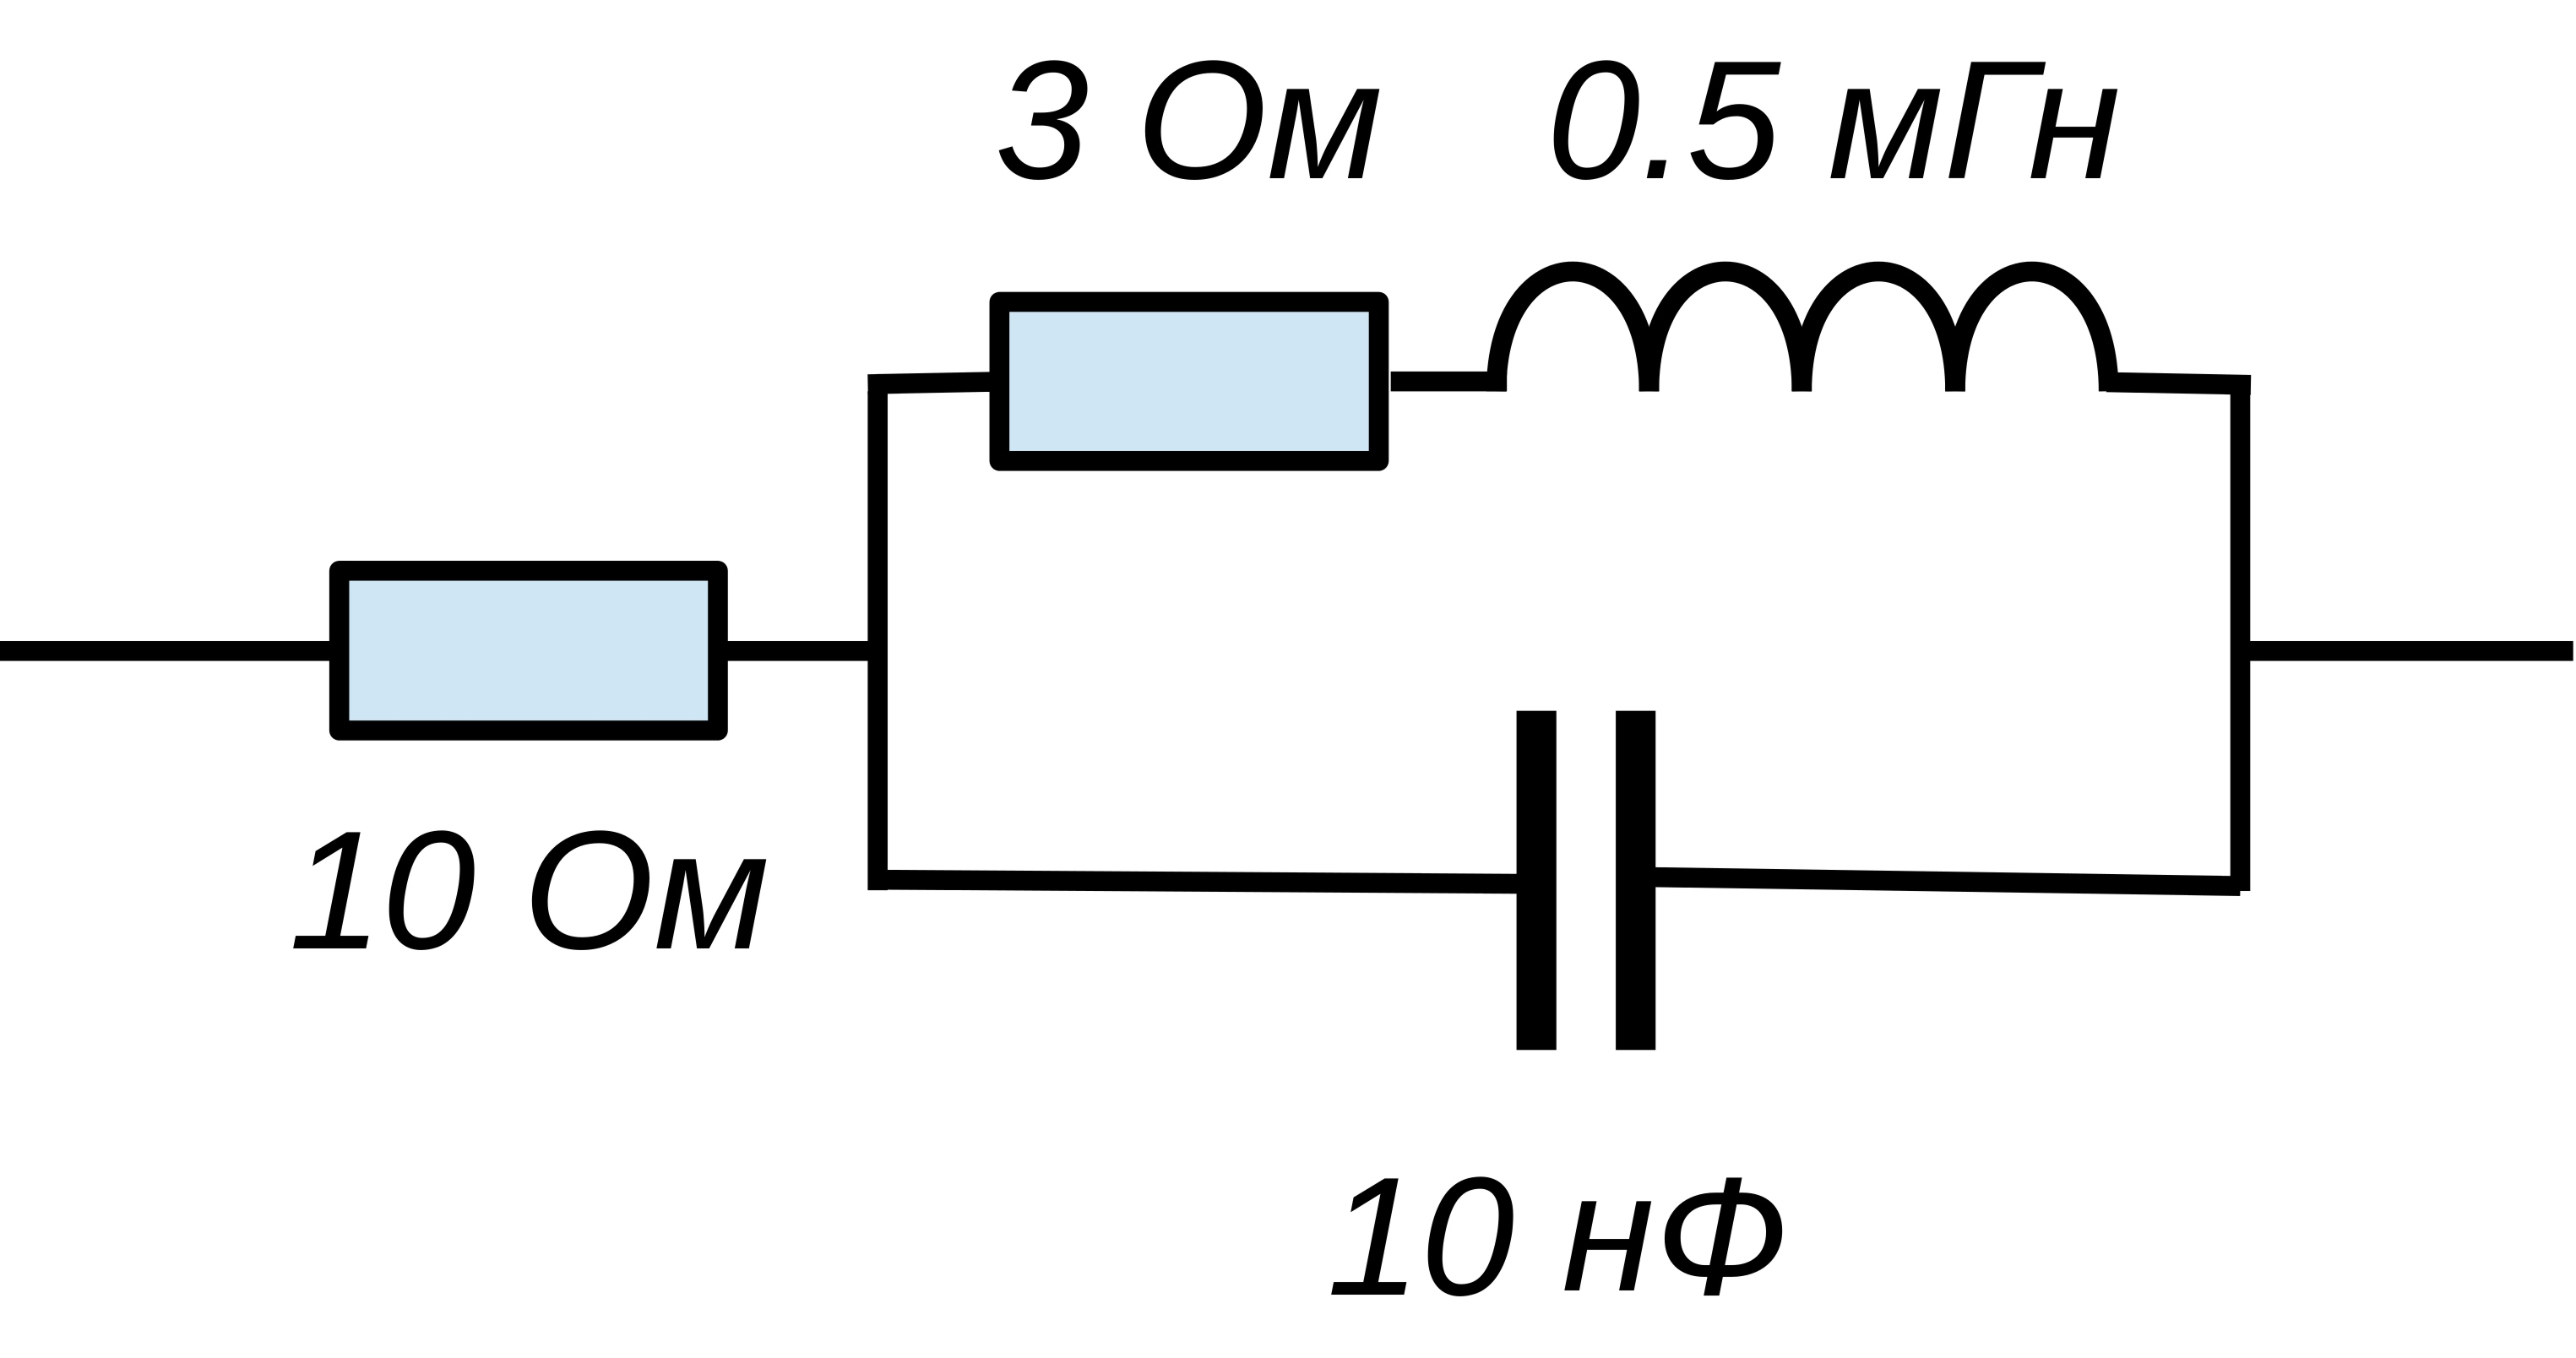
\includegraphics[width=\linewidth]{../figures/circuit.jpg}
\end{tabular}
\vspace{-\medskipamount}
\REPL{S}{'(-- (R 10) (|| (-- (R 3) (L 5e-06)) (C 10e-09)))}
\REPL{(is S Circuit)}{#t}
Символьное выражение, описывающее электрическую цепь, представляет собой обыкновенный список. Он может быть создан в программе при помощи формальных функций, а может быть считан из файла <<в готовом виде>>, как любой другой список. Таким образом, мы определили язык, пригодный для описания простых электрических цепей. Теперь нужно научиться его интерпретировать и производить расчёты.

Как известно, в~случае переменного тока, каждый из~рассмотренных нами типов элементов имеет полное сопротивление~--- \emph{импеданс}~$Z$, выражаемый комплексным числом. Действительная часть этого числа отражает активное сопротивление элемента, а мнимая --- реактивное. Для заданной частоты переменного тока в~цепи $\omega$ импедансы сопротивления $R$, индуктивности $L$, и ёмкости $C$ вычисляются следующим образом:
$$Z_R = R,\qquad Z_C = -\frac{i}{\omega C},\qquad Z_L = i\omega L.$$
А так вычисляются импедансы для последовательного и~параллельного соединения элементов цепи:
$$Z_\text{посл} = \sum\limits_i Z_i,\qquad  Z_\text{парал}= \left(\sum\limits_i\frac1{Z_i}\right)^{-1}.$$

Для представления электрических схем нужна форма записи, как для элементов, так и~для возможных типов их соединения. Мы будем использовать следующие обозначения:

\begin{itemize}
 \item[] \s{(R $x$)} для сопротивления в~$x$ ом;

 \item[] \s{(L $x$)} для катушки индуктивностью $x$ генри;

 \item[] \s{(C $x$)} для конденсатора ёмкостью $x$ фарад;

 \item[] \s{(-- $el_1$ $el_2$ ...)} для последовательного соединения элементов;

 \item[] \s{(|| $el_1$ $el_2$ ...)} для параллельного соединения.
\end{itemize}

 Интерпретатор должен по заданной цепи строить функцию, вычисляющую импеданс цепи $Z$ для заданной частоты $\omega$. 
Для наглядности, определим типы для этих величин: частота должна быть положительным действительным числом, а импеданс --- комплексным с положительной действительной частью.
\begin{Definition}
 (define-type $\omega$ positive?)
 (define-type Imp ($\circ$ real-part positive?))
\end{Definition}
Теперь мы можем записать сигнатуру и <<скелет>> функции\=/интерпретатора \s{impedance} следующим образом:
\label{example:impedance}%
\begin{SchemeCode}[emph={cir,w}]
(:: impedance (Circuit -> ($\omega$ -> Imp))
 (define (impedance cir)
   (lambda (w) ...)))
\end{SchemeCode}

В теле \lmфункции нужно определить, как вычисляются импеданс элементов и соединений. Это нетрудно сделать с помощью сопоставления с образцом. Определим вспомогательную функцию \s{Z}, которая и будет производить это сопоставление:
\newpage
\begin{Definition}[emph={cir,w,f,lst,r,c,l,i}]
(:: impedance (Circuit -> ($\omega$ -> Imp))
 (define (impedance cir)
   (lambda (w) 
     (define/. Z
       (R r) --> r
       (C c) --> (/ -i c w)
       (L l) --> (* +i l w)
       (-- i ...) --> (sum Z i)
       (|| i ...) --> (/ (sum / (map Z i))))
     (Z cir))))%\medskip%
(:: sum ((Any -> Num) list? -> Num)
  (define (sum f lst) 
    (apply + (map f lst))))
\end{Definition}
Здесь мы постарались максимально выразительно указать способ вычисления импеданса соединений через функцию \s[emph={f,lst}]{(sum f lst)}, вычисляющую сумму значений функции \lex{f} на элементах списка \lex{lst}. Внутрення \lmфункция  просто возвращает результат интерпретации входной цепи \lex{cir} функцией \s{Z}.

Теперь всё готово для расчётов:
\REPL
  {((impedance circuit) 1e6)}
  {13.027474329540581+0.4112319297625955i}

\begin{Assignment}
а) С помощью функции \s{plot} постройте график модуля импеданса цепи $S$ в диапазоне от 1\,МГц до 50\,MГц.

б) Имея функцию для импеданса какой-либо цепи, мы можем, например, вычислить резонансную частоту цепи, численно решив уравнение $\mathrm{Im} Z(\omega) = 0$.

Напишите функцию \fun{resonant-frequency}{circ $\omega_1$ $\omega_2$}, которая бы находила резонансную частоту для цепи \lex{circ} в~диапазоне частот от~$\omega_1$ до~$\omega_2$. Воспользуйтесь для решения уравнения функцией \s{bisection}, которую мы рассмотрели на~Занятии \ref{Less:recursion}  (стр.\,\pageref{bisection}).

в) Найдите при каком значении ёмкости $C$, резонансная частота цепи $S$, будет равна 20\,MГц. 

Подумайте, как с помощью мемоизации можно ускорить вычисления, не переписывая функции \s{bisection} и \s{impedance}?
\end{Assignment}

\section{Программа, \mbox{управляемая данными}}%
Существует другой весьма изящный, чисто функциональный способ решения рассмотренной нами задачи расчёта электрических цепей. Он основывается на подходе, иенуемом \emph{программированием, управляемым данными} (data-driven programming). В этом подходе стирается грань между данными и программой, так что описание данных и является обрабатывающей их программой.

Как и в предыдущей реализации будем обозначать элементы цепи функциями \s{R}, \s{C} и \s{L}. Но теперь это будут не формальные функции, а функции для расчёта импедансов отдельных элементов электрической цепи:
\begin{Definition}[emph={r,c,l,w}]
(:: R (positive? $\omega$ -> Imp)
  (define (R r w) r))

(:: C (positive? $\omega$ -> Imp)
  (define (C c w) (/ -i c w)))

(:: L (positive? $\omega$ -> Imp)
  (define (L l w) (* +i l w)))
\end{Definition}
\noindentТаким образом, например, выражение \s{(C 1e-9)} является частично\=/применённой функцией \s{C} и представляет собой функцию, имеющую сигнатуру \s{$\omega$ -> Imp}.

Функции, вычисляющие импедансы для последовательного и параллельного соединений элементов цепи должны оперировать именно такими функциями. Причём они должны комбинировать их так, чтобы в результате вновь получалась функция, пригодная к комбинированию. Ниже дана реализации этих функций, обратите внимание на их тип.
\begin{Definition}[emph={cs,c,w}]
(:: -- (($\omega$ -> Imp) .. -> ($\omega$ -> Imp))
  (define (-- . cs) 
    (lambda (w) (sum (lambda (c) (c w)) cs))))

(:: || (($\omega$ -> Imp) .. -> ($\omega$ -> Imp))
  (define (|| . cs) 
    (lambda (w) (/ (sum (lambda (c) (/ (c w))) cs)))))
\end{Definition}
Здесь мы используем такое же суммирование, как и в предыдущей реализации, но в роли интерпретирующей функции \s{Z} выступают сами комбинируемые функции.

На этом реализация интерпретатора, управляемого данными окончена. Теперь сама схема является функцией, которая <<умеет>> вычислять свой импеданс:

\begin{SchemeCode}
> (define S
    (-- (R 10)
        (|| (-- (R 3)
                (L 0.5e-6))
            (C 10e-9))))
\end{SchemeCode}
\REPL{S}{<#procedure>}
\REPL{(S 1e6)}{13.027474329540581+0.4112319297625955i}

\begin{Assignment}
 С помощью функции \sbi{time}, сравните быстродействие двух рассмотренных нами реализаций: символьной и управляемой данными.

 Какие преимущества даёт использование каждой из них?
\end{Assignment}

\section{Символьные данные \mbox{за~пределами~\Scheme}}%
Символы в~том виде, в~котором мы их использовали и~будем использовать в~наших программах, характерны для \emph{языков символьной обработки данных}. К~ним, в~первую очередь, относятся языки \Lang{SNOBOL, Refal,} \Lisp и~его диалекты.
В семействе языков \Lisp пространство имён и~пространство символов не~разделяются. Идентификатор отличается от~символа только тем, что с~ним связано некоторое значение. Это свойство делает языки семейства \Lisp по-настоящему символьными и~отличает их от~большинства других языков программирования (в том числе и~функциональных), где пространство имён переменных и~пространство символов или строк разделены.

Работа с~символами не~является специфичной для функционального программирования, но многие задачи обработки символьных данных очень изящно решаются именно в~рамках функциональной парадигмы. 

В большинстве языков программирования высокого уровня роль формальных функций играют \emph{структуры} или \emph{записи} --- именованные контейнеры, обеспечивающие доступ к своему содержимому и идентификацию структурированных данных. Однако  формальные функции являются более гибкими: они не регламентируют число и тип полей, хотя и это возможно.

В наибольшей степени, формальные функции, реализованые в \Scheme, соответствуют функциям в языка \Lang{Mathematica}. Там они так же играют роль контейнеров и идентификаторов типа, так же используются для сопоставления с образцом и для символьных вычислений.

В какой-то мере, их использование для определения типов соответствует контрукторам типов в языке \Lang{Haskell}. Существенная разница состоит в том, что в \Scheme формальные аппликации (результат применения формальных функций) представляют собой обыкновенные списки, то есть могут быть созданы любым другим способом или просто считаны из файла, однако их можно обрабатывать, как структурированные и типизированные данные с помощью сопоставления с образцом. В языке \Lang{Haskell} типизированные константы являются объектами более высокого класса.

\begin{Queeze}
 \item Какова роль символов в~языке \Scheme?

 \item Каким образом можно создать невычисленное выражение в~языке \Scheme? Как можно вычислить его целиком или частично?

 \item Чтотакое формальная функция и формальная аппликация?
\end{Queeze}

  %!TEX root = main.tex
\Lesson{Функции высшего~порядка и~функционалы}%
\label{Less:high-order}

\section[4]{Абстракция вычислительного процесса}%
В предыдущих главах мы познакомились с приёмами, хоть и характерными для функционального программирования, но успешно используемыми и вне этого подхода: рекурсия, абстрактные типы данных и символы используются в рамках самых разных парадигм. На этом занятии мы, наконец, займёмся <<настоящим>> функциональным программированием: модифицированием, комбинированием и созданием функций. 

Функциональное программирование подразумевает использование функций, как объектов первого класса, значит их можно передавать в качестве аргументов другим функциям и получать в качестве результатов.
Функция, принимающая в~качестве аргументов другие функции, называется \index{функция!высшего порядка}\emph{функцией высшего порядка}. Если функция возвращает функцию в~качестве результата, то мы будем её называть \index{функционал}\emph{функционалом}, или \index{оператор}\emph{оператором.} 

Мы уже рассматривали и~использовали функции высших порядков: \s{sum}, \s{bisection}, \s{accumulate}, \s{map} и~т.\,п. Некоторые из~них имеют достаточно узкое применение, другие используются очень широко, как универсальные инструменты. Последние являются \index{абстракция!процесса}\emph{абстракциями процессов}, обобщающими некоторые типичные вычислительные процессы. Например, функция \s{accumulate}~--- является абстракцией итерации с~накоплением в~заданном диапазоне числового индекса, \s{map}~--- отображения множества с~помощью заданной функции.

Позже мы рассмотрим ещё несколько полезных и~универсальных абстракций~--- свёртку (абстракцию структурной рекурсии), поиск неподвижной точки (к ней сводится, например, функция \s{bisection} и~вообще, произвольный рекурсивный процесс), монады, как абстракцию последовательных вычислений и~т.\,д.

В то время, как выразительная мощь и~модульность объектно-ориентированного подхода заключается в~абстракции данных, функциональная парадигма достигает этого же абстракцией процедур. Написание и~использование функций высшего порядка делает функциональные программы надёжными, модульными, расширяемыми и, при~правильном подходе, самодокументированными: прозрачными для человека. 
Однако, как и~везде, нужно уметь вовремя остановиться в~повышении уровня абстракции. Программисту необходимо помнить принцип: «Хуже обобщения одного примера может быть только обобщение вообще без~примеров»\footnote{Это один из~принципов, провозглашённых создателями оконной системы X~Windows, используемой в~UNIX-подобных системах и~в Mac OS X.}.


\section[2]{Аппликация}%
\index{аппликация}%
Одной из~самых важных функций высшего порядка является функция \sbi{apply}. Она применяет заданную функцию к последовательности или списку аргументов.

\begin{example}{%
  Примеры применения функции \s{apply}.

  Последний пример показывает, что не все аргументы нужно передавать в виде списка, однако последним аргументом функции \s{apply} должен быть список.}
  \REPLin{(define-formal f)}
  \REPL
    {(apply f '(x))}
    {(f x y)}
  \REPL
    {(apply f '(x y))}
    {(f x y)}
  \REPL
    {(apply f a b '(c))}
    {(f a b c)}
\end{example}

Эту функцию нельзя определить с~помощью других средств языка \Scheme. Процедура \emph{аппликации}, которую она осуществляет, является базовой, наряду с~процедурой \emph{абстракции},\footnote{Здесь имеется ввиду не~абстракция процесса, а~абстракция, как одна из~фундаментальных операций в~исчислении функций. Подробнее см.\,Занятие \ref{Less:lambda-calculus}, стр.\pageref{abstraction}.} реализуемой с~помощью \s{define} и~\s{lambda}.


\section{Каррирование и~сечение~функции}%
Часто бывает нужно многократно применить функцию от нескольких аргументов, при~этом зафиксировав часть из~них. Пусть, например, нам нужно увеличить все элементы списка на~единицу, или сравнить их с~числом. Мы можем решить эти задачи таким образом:

\begin{SchemeCode}
(map (lambda (x) (+ 1 x)) '(1 2 3))
(map (lambda (x) (< x 2)) '(1 2 3))
\end{SchemeCode}

\noindent%
Из бинарных функций \s{+} и~\s{<} мы с~помощью \lmфункций создали унарные функции. Абстракцией этой операции для функций произвольного количества аргументов является \emph{каррирование}.
\index{каррирование}

Функцию нескольких аргументов $f(x, y, z)$ можно представить, как несколько функций одной переменной, <<вложенных>> друг в друга:$$f(x, y, z) = x \mapsto (y \mapsto (z \mapsto f (x, y, z)))$$

Такое представление и~называется \emph{каррированием функции} нескольких переменных. Каррированная функция $f$ своему первому аргументу $x$ ставит в~соответствие функцию от~$y$ и~$z$. Если мы подставим два аргумента $x$ и~$y$, то в~результате получим функцию только от $z$. Подстановка всех трёх аргументов даёт конечный результат. Уменьшение валентности функции засчёт фиксирования некоторых её аргументов называется её \index{сечение}\emph{сечением} или \index{частичное применение}\emph{частичным применением}.

Мы уже встречались с усечёнными и каррированными функциями, когда рассматривали задачу расчёта импеданса электрических цепей. Посмотрите на сигнатуру функции \s{impedance} (стр.~\pageref{example:impedance}): она определена каррированной, для того чтобы для заданной цепи возвращать функцию, вычисляющую импеданс. Функциональное решение также использовало принципы каррирования. Бинарные функции \s{R}, \s{C} и \s{L}, вызываемые с одним агрументом, превращались в сечения --- унарные функции, преобразующие частоту в импеданс.

\label{ML-notation}\index{нотация!бесскобочная}В очень многих функциональных языках программирования все функции каррированы и~это позволяет обходиться без~функциональных скобок при~их применении. В языке \Scheme разрешён упрощённый синтаксис для сечения функций, таким образом, и в нём все функции можно воспринимать, как каррированные.

\begin{Assignment}

  а) Напишите определение для функционала \fun{curry}{f xs \ddd}, который возвращал бы сечение функции \lex{f}, фиксируя аргументы \lex{xs \ddd}. 

  \begin{Specification}
(test
  (map (curry * 2) '(1 2 3)) ==> '(2 4 6)  ;$(2\times1\ 2\times2\ 2\times3)$
  (map (curry - 2) '(1 2 3)) ==> '(1 0 -1) ;$(2-1\ 2-2\ 2-3)$
  ((curry list 1 2) 3 4)     ==> '(1 2 3 4))
  \end{Specification}

  б) Для некоммутативных операций не~всё равно, какой аргумент отбрасывается при~сечении. При использовании функционала \s{curry}, аргументы каррированной функции фиксируются «слева». Напишите функционал \si{curryr}, фиксирующий фаргументы «справа»: 

  \begin{Specification}
(test 
  (map (curryr - 2) '(1 2 3)) ==> '(-1 0 1)   ;$(1-2\ 2-2\ 3-2)$   
  (map (curryr < 2) '(1 2 3)) ==> '(#t #f #f)
  ((curryr list 1 2) 3 4)     ==> '(3 4 1 2))  
  \end{Specification}
\end{Assignment}

\section{Композиция функций}%
\index{композиция функций}%
\emph{Композицией} называется такая комбинация двух функций, что результат одной из них подставляется в~качестве аргумента другой. Математически это записывается так:$$(f \circ g)(x) = f(g(x))$$
Композиция является \emph{абстракцией комбинирования функций}: с~её помощью мы можем порождать новые функции не~используя явных связываний и~формальных аргументов.

В языках \Scheme и \Lang{Haskell} функции каррированы, это позволяет обобщить понятие композиции  для функций нескольких переменных. Рассмотрим, например, как можно свести к композиции следущее выражение, записанное в префиксной нотации:
$$(f~(g~x)~y).$$
Если считать бинарную функцию $f$ каррированной, то выражение можно переписать так:
$$((f~(g~x))~y),$$
при этом к аргументу \lex{y} применяется функция $(f~(g~x))$, которую можно представить, как: $((f\circ g)~x)$, опять же, при условии, что и функция $f$ и композиция каррированы. Таким образом, исходное выражение переписывается следущим образом: $$(((f \circ g)~x)~y) = ((f \circ g)~x~y).$$

\newpage
\begin{Assignment}
a) Определите функцию \s{compose}, возвращающую композицию произвольного числа унарных функций:
\begin{Specification}
(test
  ((compose sqr +) 1 2 3)           ==> 36
  ((compose list list sqr +) 1 2 3) ==> '((36))
  ((compose +) 1 2 3)               ==> 6)
\end{Specification}

б) Опертор композиции функций должен удовлетворять следующим свойствам:
\begin{itemize}
  \item \emph{ассоциативность}: $(f \circ g) \circ h = f \circ (g \circ h)$,
  \item \emph{наличие нейтрального элемента}: $f \circ id = id \circ f = f$.
\end{itemize}
Здесь \s{id} --- тождественная функция.
Проверьте, удовлетворяют ли этим свойствам написанный вами вариант оператора \s{compose} и обобщённая композиция $\circ$\footnote{Символ $\circ$ может быть введён, как \s{\\circ} + \MenuItem{Alt} \s{\\}}. Рассмотрите  композицию функций различной валентности.
\end{Assignment}


\section{Некоторые полезные функционалы}\label{operators}%
В арсенале функционального программирования существует много полезных операторов и функционалов, позволяющих комбинировать и модифицировать функции. В примерах к этому разделу будут использоваться формальные функции \s{f} и \s{g}.

\medskip
\fun{const}{C}~--- тождественная функция, возвращающая значение константы \lex{C} для любых аргументов.

\REPL
  {((const 5) 1 2)}
  {5}

% \REPL
%   {(map (const 'a) '(2 9 0))}
%   {(a a a)}

\medskip
\fun{arg}{n}~--- тривиальная функция, возвращающая \lex{n}-ный переданный ей аргумент.
\REPL
  {((arg 2) 'x 'y 'z)}
  {y}

Через функцию \s{arg} выражаются два часто встречающиеся оператора \si{I1} и \si{I2}:
\begin{SchemeCode}
  I1 = (arg 1),   I2 = (arg 2).
\end{SchemeCode}

\medskip
\fun{flipped}{f} -- возвращает функцию, эквивалентную $f$, но принимающую аргументы в обратном порядке.
\REPL
  {((flip f) 1 2)}
  {'(f 2 1)}

\medskip
\fun{fif}{test? f g}~--- оператор выбора функции по~функции\=/предикату. Все функции\=/аргументы этого оператора получают одинаковые аргументы.
\REPL
 {(map (fif even? f g) '(1 8 13 4))}
 {'((g 1) (f 8) (g 13) (f 4))}

\medskip
\fun{andf}{p q \ddd}, \fun{orf}{p q \ddd} и \fun{negated}{p}~--- операторы конъюнкции, дизъюнкции и отрицания предикатов.
\REPL
  {(filter (andf integer? (> 3)) '(2.5 -6 4 2 12))}
  {'(-6 2)}
\REPL
  {(map (negated <) '(1 2 3 4) '(3 3 3 3))}
  {'(#f #f #t #t)}

\medskip
\fun{argmap}{f g} --- оператор, применяющий перед аппликацией функции \lex{f} унарную функцию \lex{g} к её к аргуметам.
\REPL
  {((argmap f g) 'x 'y 'z)}
  {'(f (g x) (g y) (g z))}

\begin{Assignment}
Напишите определения для операторов \s{const}, \s{arg}, \s{flipped}, \s{fif}, \s{andf}, \s{orf}, \s{negated} и \s{argmap}. Дайте спецификацию их типа.
\end{Assignment}

\section[2]{Бесточечная нотация}\index{нотация!бесточечная}\label{tacit}%
Часто, при определении функции нет необходимости описывать, как она действует на~свои формальные аргументы. Вместо этого можно дать определение её действию в~целом.

Например, давая определение предикату \si{atom?}, который проверяет, является ли объект элементарным или составным, мы можем написать прямое определение:

\begin{SchemeCode}[emph=x]
(define (atom? x) 
  (not (pair? x)))
\end{SchemeCode}
\noindent или определение, использующее оператор \s{negated}:
\begin{SchemeCode}[emph=x]
(define (atom? x) 
  ((negated pair?) x))
\end{SchemeCode}
\noindent при~этом мы видим, что формальный аргумент \lex{x} никакой информации этому определению не~добавляет и~его можно опустить:
\vspace{-\bigskipamount}
\begin{SchemeCode}
(define atom? (negated pair?))
\end{SchemeCode}
\noindent Это пример определения, записанного в~\emph{бесточечной нотации}.

\label{union}Приведём ещё один простой пример. Посмотрите на~определение функции, возвращающей объединение двух множеств, представленных списками:
\begin{SchemeCode}[emph={s1,s2}]
(define (union s1 s2)
  (remove-duplicates (append s1 s2)))
\end{SchemeCode}
\noindent Видно, что мы передаём аргументы сначала функции \s{append}, которая объединяет два списка-множества в~один, а~потом результат передаём функции \s{remove-duplicates}. Она, в~свою очередь, выделяет множество элементов этого списка, удаляя дубликаты. Поток данных можно схематически показать так:
\begin{center}
\s{s1, s2  $\longrightarrow$  append  $\longrightarrow$  remove-duplicates}
\end{center}

\noindent С~точки зрения функционального программирования, мы имеем композицию функций \s{append} и~\s{remove-duplicates}. Следовательно, мы можем дать следующее определение операции объединения:

\begin{SchemeCode}
(define union ($\circ$ remove-duplicates append))
\end{SchemeCode}

Это именно определение функции, поскольку композиция является функцией, но указывать её формальные аргументы не~требуется. Более того, нам даже не~нужно указывать их количество, поскольку функция \s{append} обрабатывает любое число аргументов, наша функция \s{union} будет обладать таким же свойством!

\begin{example}{Функция \s{union} может работать с~любым количеством аргументов.

Попробуйте вызвать её с~одним аргументом или вовсе без~них.}
\REPL
  {(union '(1 2 3) '(2 3 4))}
  {(1 2 3 4)}

\REPL
  {(union '(a b c) '(1) '(b))}
  {(a b c 1)} 
\end{example}

Важную роль в бесточечном определении функций играет каррирование. Например, имея функцию \s{accumulate} (стр. \pageref{accumulate}), мы можем определить функцию \s{sumf}, вычисляющую $\sum_{i=a}^b f(i)$,  следующим образом:
\begin{SchemeCode}[emph={f,a,b}]
  (define (sumf f a b) (accumulate + 0 f a b))
\end{SchemeCode}
или с помощью сечения:
\begin{SchemeCode}
  (define sumf (accumulate + 0))
\end{SchemeCode}
При этом имеется в виду, что свободные аргументы \lex{f a b} становятся аргументами функции \s{sumf}. Это лаконичное определение очень точно отражает суть определяемой функции: сумма -- это аккумуляция с операцей сложения и нулём в качестве нейтрального элемента.

Так можно определить функцию, вычисляющую $\sum_{i=a}^b i^2$. Зафиксировав первый аргумент функции \s{sumf}, мы оставляем пределы суммирования свободными.
\begin{SchemeCode}
   > (define sumsq (sumf sqr))
\end{SchemeCode}
\REPL
  {(sumsq 1 3)}
  {14} 

В языке \Scheme для определений функций с использованием каррирования служит форма \sfi{define/c}:\label{define-c} 
\begin{SchemeCode}
(define/c (f x y ...) body).
\end{SchemeCode}
Выражение \s{(f x y ...)} представляет собой сечение определяемой функции \s{f}. При этом, если выражение \s{body} возвращает функцию, то её формальные аргументы становятся свободными аргументами функции \s{f}.

Вот, как с помощью формы \s{define/c}, можно определить функцию \s{map}:
\begin{SchemeCode}[emph={f,h,t}]
(define/c (map f)
  (/. '() --> '()
      (cons h t) --> (cons (f h) (map f t))))
\end{SchemeCode}
В заголовке этого определения мы зафиксировали первый аргумент функции \s{map}, оставив свободными аргументы функции, заданной подстановкой. Так как подстановка является унарной, то в результате, мы получаем бинарную функцию:
\REPL
  {(map sqr '(1 2 3))}
  {(1 4 9)} 

Бесточечная нотация делает функциональные программы более декларативными. Вместо описания функции, как последовательности действий над~аргументами, она описывает, чем является эта функция по~отношению к~другим функциям.

Бесточечный стиль характерен для функциональных языков и~широко используется в~языках семейства \Lang{ML}. Однако нужно уметь «вовремя остановиться», используя его. Основная цель такой записи~--- повысить понятность кода и~его надёжность. Однако, используя бесточечный стиль, очень легко превратить программу в~бессмысленный, на~первый взгляд, набор функций и~комбинаторов. Рекомендуется применять бесточечную запись только тогда, когда она чётко и~ясно отражает структуру определяемой функции, приближая определение к~словесному описанию.

\section[4]{Функции высшего~порядка \mbox{за~пределами~\Scheme}}%
Функции высшего порядка можно создавать и~использовать во~всех языках, которые позволяют передавать качестве аргументов функций другие функции или указатели на~них.
Во всех функциональных языках функции~--- объекты первого класса и~создание функций высшего порядка для них естественно.

В языке \Lang{С++} можно создавать такие функции с~помощью указателей на~функции. В~языке \Lang{Pascal} (\Lang{Delphi}) и~прочих объектно-ориентированных языках можно передавать функцию, как метод объекта.

\index{замыкание}Важным инструментом для создания функций высшего порядка является механизм замыкания, который позволил нам описать каррирование функций. Замыкание присутствует во~многих языках: \Lang{С++} использует для этого функторы или блоки; \Lang{Delphi}, \Lang{Perl}, \Lang{Python} и~\Lang{JavaScript}~--- анонимные функции, \Lang{Java}~--- использует анонимные классы внутри методов.

\begin{Queeze}

\item Какая функция называется функцией высшего порядка? Приведите примеры.

 \item Какую роль играют функции высшего порядка и~функционалы в~программировании?

 \item Абстракцией какого процесса является оператор \s{fif}?

 \item Какие функции являются абстракциями комбинирования функций, аппликации функций, частичного применения, рекурсивного обхода древообразной структуры?

 \item Что такое бесточечная нотация?

\end{Queeze}
  % %!TEX root = main.tex
\Lesson{Функция свёртки}%
\label{Less:fold}

\section[2]{Правая свёртка}%
Важным аспектом программирования является возможность обобщать различные вычислительные процессы, выделяя в~них общую схему вычислений. Мы уже делали это, разрабатывая функцию \s{accumulate,} к~которой сводятся функции \s{sum}, \s{product}, \s{table} и~т.\,д.

Многие функции, обрабатывающие списки имеют одинаковое функциональное <<ядро>>, соответствующее структурной рекурсии, которое можно выделить в форме абстрактной функции обработки списочных структур. 

В качестве примера, рассмотрим определения трёх функций, которые последовательно обрабатывают элементы списка.
Функция \fun{total}{lst} складывает элементы заданного списка; функция \fun{any}{p lst} выясняет, есть ли в списке хотя бы один элемент, удовлетворяющий предикату \lex{p}; и, наконец, функция \fun{map}{f lst} осуществляет отображение списка:
\begin{SchemeCode}[emph={lst,x}]
(define total
  (/. '() --> 0
      (cons h t) --> (+ h (total t))))

(define/c (any p)
  (/. '() --> #f
      (cons h t) --> (or (p h) (any p t))))

(define/c (map f)
  (/. '() --> '()
      (cons h t) --> (cons (f h) (map f t))))
\end{SchemeCode}

Чтобы выделить существенную часть в определениях этих функций, мы использовали форму \s{define/c}, которая позволяет оперировать функциями, как если бы они были каррированы (cм.~стр.~\pageref{define-c}). Таким образом, функция \s{any} имеет два аргумента~--- предикат \lex{p}, заданный в левой части определения, и список~--- аргумент функции\=/подстановки.

Рассмотренные нами три функции имеют очень похожую структуру~--- для некой бинарной функции $f$ и~некоего «нулевого» элемента $x_0$ определяется функция $F$ по~следующей схеме:
\begin{SchemeCode}[emph={lst,x}]
(define F
  (/. '() --> $x_0$
      (cons h t) --> ($f$ h ($F$ t))))
\end{SchemeCode}
\noindent%
Отличаются У этих трёх функций только $f$ и~$x_0$:

\begin{center}
\begin{threeparttable}
\begin{tabular}{>{\schemestyle}llc}\toprule
\multicolumn{1}{c}{$F$} & \multicolumn{1}{c}{$f$} & $x_0$\\\midrule
total & $x, y \rightarrow  x + y$ & \constantstyle 0\\
any & $x, y \rightarrow  (or~(p~x)~y)$ & \constantstyle{\#f}\\
map & $x, y \rightarrow  ((f~x)\ .\ y)$ & \schemestyle '()\\\bottomrule
\end{tabular}
\end{threeparttable}
\end{center}

Выделим функциональное ядро этих функций и~назовём его \index{свёртка!списка! правая}\emph{правой свёрткой}:\label{foldr}

\fnindex{foldr}
\begin{SchemeCode}[emph={f,h,t}]
(:: foldr ((A B -> B) B (list: A ..) -> B)
 (define/c (foldr f $x_0$)
   (/. '() --> $x_0$
       (cons h t) --> (f h (foldr f $x_0$ t))))
\end{SchemeCode}

Обратите внимание на~описание типа функции \s{foldr}. Первым её аргументом должна быть сворачивающая функция двух аргументов, вторым~--- «нулевой» элемент, а~третьим~--- список. При~этом типы элементов списка и~«нулевого» элемента должны соответствовать типам аргументов сворачивающей функции. На~выходе мы получаем результат того же типа, что возвращает сворачивающая функция.

Фактически, эта рекурсивная функция, применённая к~некоему списку, выполняет следующее преобразование:
\begin{SchemeCode}[emph=f]
        (foldr f $x_0$ '(a b c)) $\rightarrow$ (f a (f b (f c $x_0$)))
\end{SchemeCode}
Иными словами, для списка \s{'(a b c)} функция \s{foldr} делает формальную замену: \s[emph=f]{cons $\rightarrow$ f}, \s{null $\rightarrow$ $x_0$}
так, что получается преобразование:
\begin{SchemeCode}[emph=f]
    (cons a (cons b (cons c '()))) $\rightarrow$ (f a (f b (f c $x_0$)))
\end{SchemeCode}

\newpage\noindent
Например, для рассмотренных нами функций:

\begin{SchemeCode}
total:  
 cons $\rightarrow$ +,  '() $\rightarrow$ 0  
 (a . (b . (c . '()))) $\rightarrow$ (a + (b + (c + 0)))%\smallskip%
any: 
 cons $\rightarrow$ (lambda (x y) (or (p x) y)), '() $\rightarrow$ #f  
 (a . (b . (c . '()))) $\rightarrow$ (or (p a) (or (p b) (or (p c) #f)))%\smallskip%
map:
 cons $\rightarrow$ (lambda (x y) (cons (f x) y)), '() $\rightarrow$ '() 
 (a . (b . (c . '()))) $\rightarrow$ ((f a) . ((f b) . ((f c) . '())))
\end{SchemeCode}

Теперь мы можем выразить наши три рекурсивные функции через правую свёртку:

\begin{Definition}[emph={lst,x,y,lst1,lst2,p}]
(define (total lst)
  (foldr + 0 lst))%\medskip%
(define (any p lst)
  (foldr (lambda (x y) (or (p x) y)) #f lst))%\medskip%
(define (map lst1 lst2)
  (foldr (lambda (x y) (cons (f x) y))  lst1)) 
\end{Definition}

С помощью операторов, описанных на стр.~\pageref{operators} и бесточечной нотации (стр.~\pageref{tacit}), удобно давать чисто операторные определения функциям, использующим свёртку:

\label{fold:map}
\begin{Definition}[emph={f,p,test?}]
(define/c (total)  (foldr + 0))%\medskip%
(define/c (any p)  (foldr ($\circ$ or p) #f))%\medskip%
(define/c (map f)  (foldr ($\circ$ cons f) '()))%\medskip%
\end{Definition}

Такие определения не~всегда улучшают читаемость программы, однако они повышают её модульность, что увеличивает надёжность, упрощает отладку программы и~доказательство её корректности.

При~разработке функции, использующей свёртку, полезно мыслить по~следующей схеме: представляем себе исходный список в~виде цепочки вложенных пар: \s{(a . (b . (c . '())))} и~решаем, что мы должны сделать с~каждым элементом списка, на~что мы заменим операцию \s{(.)} и~с чего начинать свёртку. Функция с~помощью которой мы сворачиваем список имеет два аргумента: первый~--- это текущий элемент списка, второй~--- текущий результат свёртки.

Например, мы хотим написать функцию, возвращающую сумму квадратов всех элементов списка. Значит, мы должны сделать преобразование: 
\textrm{\normalfont($a$ . ($b$ . ($c$ . '()))) $\rightarrow$  $a^2$ + ($b^2$ + ($c^2$ + 0))}.  
Сворачивающая функция может выглядеть так:  $f(el,res) = el^2+res$.

\begin{Assignment}
Напишите, используя свёртку, определения следующих функций:

 а) \fun{every}{test? lst} --- возвращает \s{#t} тогда, когда все элементы списка \lex{lst} удовлетворяют предикату \lex{test?}.\vspace{-\smallskipamount}
\begin{Specification}
(test (every odd? '(1 3 5))
      (not (every odd? '(1 2 3))))
\end{Specification}

 б) \fun{count-if}{test? lst} --- подсчитывает число вхождений в список \lex{lst} элементов, удовлетворяющих предикату \lex{test?}.\vspace{-\smallskipamount}
\begin{Specification}
(test (count-if odd? '(1 2 3))  ==> 2
      (count-if odd? '(0 2 4))  ==> 0
      (count-if odd? '())       ==> 0)
\end{Specification}

 в) \fun{count}{el lst} --- подсчитывает число вхождений элемента \lex{el} в~список \lex{lst}. Здесь воспользуйтесь функцией \s{count-if}, написанной вами ранее. \vspace{-\smallskipamount}
\begin{Specification}
(test (count 1 '(2 1 2 1 1))  ==> 3
      (count 3 '(2 1 2 1 1))  ==> 0
      (count 3 '())           ==> 0)
\end{Specification}
\end{Assignment}

\section[2]{Левая свёртка}\index{свёртка!списка!левая}%
Рассмотрим, как может быть реализована функция \si{reverse}, возвращающая список с~элементами, данными в~обратном порядке. Вспомним, что вычисление правой свёртки начинается с~конца списка. Значит, если мы будем сворачивать список функцией \s{appendr}:
\begin{SchemeCode}[emph={x,lst}]
(define (appendr x lst)
  (append lst (list x)))
\end{SchemeCode}

\noindentто каждый следующий элемент будет приклеиваться к~результату справа и~мы получим то, что нужно:

\begin{SchemeCode}
(a . (b . (c . '()))) arrow
arrow (append (append (append '() '(c)) '(b)) '(a)) arrow
arrow (c . (b . (a . '())))
\end{SchemeCode}

Таким образом, получаем определение:

\begin{Definition}
(define (reverse lst)
  (foldr appendr '() lst))
\end{Definition}

Однако эта функция неэффективна: она, проходя по~списку, вынуждена проходить по~каждому вызову \s{append} все достраиваемые подсписки. Таким образом, для списка из~$N$ элементов эта функция совершает $N^2/2$ операций \s{cons}. Вот если бы свёртка осуществлялась не~с конца, а~с начала списка, то можно было бы обойтись использованием только функции \s{cons}. Напишем такую функцию свёртки:

\fnindex{foldl}
\begin{Definition}[emph={f,h,t}]
(:: foldl ((A B -> B) B (list: A ..) -> B)
 (define/c (foldl f $x_0$)
   (/. '() --> $x_0$
       (cons h t) --> (foldl f (f h $x_0$) t))))
\end{Definition}

\noindent
Она выполняет следующее преобразование:

\begin{SchemeCode}
      (foldl $f$ $x_0$ '(a b c))  $\rightarrow$  ($f$ c ($f$ b ($f$ a $x_0$)))
\end{SchemeCode}

\noindent Заметим, что список сворачивается слева направо, поэтому такая свёртка называется \emph{левой}. Обратите так же внимание на~то, что левая свёртка реализует итеративный процесс.

С помощью левой свёртки, функция \s{reverse} выражается очень просто и эффективно:
\begin{SchemeCode}
(define reverse (foldl cons '()))
\end{SchemeCode}

\begin{Assignment}
Определите через свёртку следующие универсальные функции:

\s{(length $lst$)} --- возвращает длину списка $lst$.

\s{(max $lst$)} --- возвращает максимальный элемент списка $lst$.

\fun{filter}{test? lst}~--- фильтрует список \lex{lst}, оставляя в~нём только те элементы, которые удовлетворяют условию \lex{test?}.
\medskip

 \fun{append}{lst1 lst2}~--- объединяет списки \lex{lst1} и \lex{lst2} в один.
\medskip

 \fun{member?}{el lst}~--- отвечает на~вопрос: содержит~ли список \lex{lst} элемент \lex{el}?
\medskip

 \fun{compose}{f \ddd}~--- композиция произвольного числа функций. При этом самая правая функция может принимать сколько угодно аргументов, а прочие~--- унарны.
\medskip

\label{remove-duplicates} \fun{remove-duplicates}{lst}~--- возвращает список уникальных элементов списка \lex{lst}.
\medskip

\fun{from-digits}{digit-list base}~--- возвращает целое число в десятичной системе исчисления, состоящее из~цифр, перечисленных в~списке \lex{digit-list}, используя основание \lex{base}. Если основание не задано, функция должна использовать десятичную систему.
\begin{Specification}
(test 
  (from-digits '(1 2 3))     123  ;основание 10
  (from-digits '(1 0 0) 2)   4)   ;основание 2
\end{Specification}
\end{Assignment}

\section{Абстракция структурной~рекурсии}%
Мы увидели, что через свёртку можно выразить множество разнообразных функций, обрабатывающих списки. Такая универсальность не случайна. Вспомним, как определяется абстрактный тип для списков:
\begin{SchemeCode}
(define-type List 
  '()
  (cons: Any List))
\end{SchemeCode}

\noindent
Абстрактные типы, построенные таким образом, называют \index{тип!алгебраический}\emph{алгебраическими}. Они определяются, через \emph{суммы} и \emph{произведения} типов. Сумма типов представляется с помощью объединения, а в качестве операции <<перемножения>> может выступать любая функция\=/констуктор, имеющая более одного агрумента. В случае типа \s{List} --- это сумма единичного типа \s{'()} и произведения типов \s{Any} и \s{List}, выполненного с помощью конструктора \s{cons}.

Определение любой структурно-рекурсивной функции обязательно должно содержать в себе правила для всех слагаемых обрабатываемого алгебраического типа и рекурсивные вызовы. Свёртка является наиболее общей структурно-рекурсивной функцией, описывающей что делать со всеми слагаемыми и множителями в произведениях типов, и вызывающая саму себя для рекурсивных множителей.
Таким образом, она является \emph{абстракцией структурной рекурсии}, и значит, её можно определить для всякого индуктивного множества. 

В качестве примера, построим свёртку для множества натуральных чисел, тип для которых формально можно записать так:
\vspace{-\bigskipamount}
\begin{SchemeCode}
(define-type Nat
  0
  (+ 1 Nat))
\end{SchemeCode}

\noindent
Нам необходимо описать обработку базового случая \s{0} и произведения \s{(+ 1 Nat)}:
\begin{Definition}
(:: nat-fold ((Nat A -> A) A Nat -> A)
  (define/c (fold-nat f x0)
    (/. 0 --> x0
        (+ 1 x) --> (f (+ 1 x) (nat-fold f x0 x)))))
\end{Definition}

\begin{example}{%
Посмотрим, как работает эта функция:}
\REPLin{(define-formal f g)}
\REPL
  {(fold-nat f 'x0 3))}
  {'(f 3 (f 2 (f 1 x0)))}
\end{example}

Использование свёртки увеличивает модульность программы, гарантирует завершаемость и корректность обработки данных принадлежащих к алгебраическим типам.

\section[2]{Свёртка деревьев}%
\index{свёртка!дерева}
В~самом общем случае, любые заквотированные выражения представляют собой списки списков, то есть, древообразные структуры, или просто \emph{деревья}. Структуру такого дерева можно показать следующим образом: в~узлах находится конструктор \s{cons}, а~листьями являются атомы. На левом рисунке показано дерево, соответствующее выражению \s{'((a (b)) (c d e))}.
\begin{center}\label{fig:tree}
  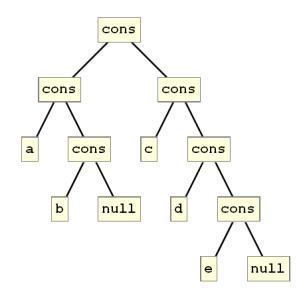
\includegraphics[width=0.43\textwidth]{../figures/tree1.jpg}
  \qquad
  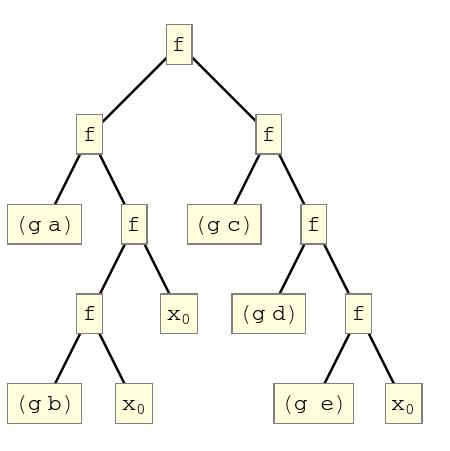
\includegraphics[width=0.43\textwidth]{../figures/tree4.jpg}
\end{center}

Так как \s{cons}~--- бинарная функция, из каждого узла может выходить только две ветви. Такие деревья называются \emph{бинарными}. 

Определим тип для бинарного дерева следующим образом:
\begin{Definition}
(define-type (BTree A)
  '()
  (cons: (BTree A) (BTree A))
  A)
\end{Definition}

Имея выражение для типа, можно сразу дать определение свёртки для него, описав, что делать с каждым слагаемым, и организуя рекурсивные вызовы для рекурсивных множителей в произведении типов:
\fnindex{foldt}
\begin{Definition}[emph={f,g,a,l,r}]
(:: foldt ((A A -> A) (Any -> A) A (BTree Any) -> A)
 (define/c (foldt f g $x_0$)
   (/. '() --> $x_0$
       (cons l r) --> (f (foldt f g $x_0$ l) 
                        (foldt f g $x_0$ r))
       a --> (g a)))
\end{Definition}
Результат свёртки выражения \s{'((a (b)) (c d e))} показан на правом рисунке на стр.~\pageref{fig:tree}.

Теперь мы можем написать, например, расширения на~случай деревьев для функций \s{length} и~\s{total}: назвав их, соответственно, \si{leaf-count} и~\si{leaf-total}:

\begin{SchemeCode}
(:: leaf-count ((BTree Any) -> Nat)
 (define leaf-count 
   (foldt + (const 1) 0)))

(:: leaf-total ((BTree Num) -> Num)
 (define leaf-total 
   (foldt + id 0)))
\end{SchemeCode}

Вот --- определение функции \si{flatten}, возвращающей список листьев дерева:
\begin{SchemeCode}
(:: flatten ((BTree Any) -> list?)
 (define flatten 
   (foldt append list '())))
\end{SchemeCode}

\newpage
\begin{Assignment}
а) Выразите через свёртку натуральных чисел \s{fold-nat} функцию \s{accumulate} (Задание \ref{accumulate}, стр.~\pageref{accumulate}).

б) Напишите определения следующих универсальных функций для деревьев:

 \fun{leaf-map}{f tree}~--- возвращает дерево \lex{tree}, ко~всем листьям которого применяется функция \lex{f}.
\begin{Specification}
; leaf-map :: (A \arrow B) Tree(A) \arrow Tree(B)
(test 
  (leaf-map sqr '((1 2) (3 (4))))  '((1 4) (9 (16)))
  (leaf-map odd? '(1 (2 (3) 2) 1)) '(#t (#f (#t) #f) #t)
  (leaf-map list '(1 2 3))         '((1) (2) (3))
  (leaf-map list 3)                '(3)
  (leaf-map sqr '(1. 12))          '(1. 144))
\end{Specification}

 \fun{find}{test? tree}~--- возвращает список листьев дерева \lex{tree}, которые удовлетворяют условию \lex{test?}.
\begin{Specification}
; find :: (A \arrow Bool) Tree(A) \arrow [A]
(test 
  (find odd? '(1 (2 (3) 2) 1))   '(1 3 1)
  (find odd? '(1 2 3 4))         '(1 3)
  (find zero? '(1 (2 (3) 2) 1))  '())
\end{Specification}

\fun{filter}{test? tree}~--- возвращает дерево с~той же структурой, что и~\lex{tree}, но в~котором присутствуют только листья, удовлетворяющие условию \lex{test?}.
\begin{Specification}
; filter :: (A \arrow Bool) Tree(A) \arrow Tree(A)
(test 
  (filter odd? '(1 2 3 4))              '(1 3)
  (filter odd? '((1 2) (3 4)))          '((1) (3))
  (filter odd? '(0 (1 (2 (3 4)))))      '((1 ((3))))
  (filter negative? '(0 (1 (2 (3 4))))) '(((())))
  (filter odd? 6)  #f)
\end{Specification}

в) Напишите функцию свёртки для типа <<размеченное дерево>>:
\begin{SchemeCode}
    Tree(A) ::= Empty
             |  Node(A, Tree(A), Tree(A))
\end{SchemeCode}
\end{Assignment}


\newpage
\begin{Assignment}
\label{as:set}Дайте определения следующим операциям теории множеств:

\fun{element?}{x s}~--- определяет является ли \lex{x} элементом множества \lex{s};

\fun{set}{lst}~--- возвращает множество элементов списка \lex{lst};

\fun{subset?}{s${}_1$ s${}_2$}~--- определяет является ли множество \lex{s${}_1$} подмножеством \lex{s${}_2$};

\fun{union}{s${}_1$ s${}_2$}~--- объединение двух множеств;

\label{intersection}\fun{intersection}{s${}_1$ s${}_2$}~--- пересечение двух множеств;

\label{complement}\fun{complement}{s${}_1$ s${}_2$}~---  множество, в~которое входят все элементы первого множества, не~входящие во~второе.
\end{Assignment}

\section{Свёртка \mbox{за~пределами \Scheme}}%
Свёртка списочных структур включена в~базовые или библиотечные функции многих языков программирования.

\medskip
\begin{tabular}{>{\smallskip\slshape}l>{\schemestyle}l}
C\#
&
{\syntaxform ienum.Aggregate}(x0, func )\\

C++
&
{\syntaxform std::accumulate}(begin, end, x0, func)\\

JavaScript
&
{\syntaxform array.reduce}(func, x0)\\

Perl 6
&
{\syntaxform reduce} block x0, list\\

PHP
&
{\syntaxform array\_reduce}(array, func, x0)\\

Python
&
{\syntaxform functools.reduce}(func, list, x0)
\end{tabular}
\medskip

В том или ином виде, свёртка входит в~число базовых функций во~все функциональные языки программирования.

\begin{Queeze}
  \item Что такое «свёртка»? Где и~как она используется?
  \item Чем отличаются правая и~левая свёртки списков?
  \item Как связаны свёртка дерева и~свёртка списков?
\end{Queeze}

  % %!TEX root = main.tex
\Lesson{Отложенные вычисления}\label{Less:delayed-computation}

\section[4]{Аппликативный и~нормальный порядок вычисления}%
\label{normal-order}Мы уже рассказывали, каким образом интерпретатор \Scheme вычисляет выражения: сначала вычисляются оператор и~операнды, а~затем получившаяся процедура применяется к~получившимся аргументам (см. Занятие \ref{Less:functions}, стр.\,\pageref{applicative-order}).

Существует и~другая модель, в~которой вычисление аргументов не~производится до~тех пор, пока не~понадобится их значение. Вместо этого в~функцию подставляются выражения-операнды, до~тех пор пока не~получится выражение, в~котором присутствуют только элементарные операторы, и~лишь затем производится вычисление всего выражения. Этот второй метод известен под~названием \index{порядок вычисления!\emph{нормальный}}\emph{нормальный порядок вычислений}.

Вычисления, основывающиеся на~аппликативном порядке называются \index{вычисления!интенсивные}\emph{интенсивными}, а~на нормальном~--- \index{вычисления!ленивые}\emph{ленивыми}. Существуют \index{языки программирования!\emph{ленивые}}\emph{ленивые языки программирования} в~которых используется только нормальный порядок вычислений. Ярким примером таких языков является язык \Lang{Haskell}.

\section[2]{Специальные формы}\index{специальная форма}%
В языке \Scheme преимущественно используется аппликативный порядок. Но никакой язык программирования не~сможет обойтись только им. 

Рассмотрим, для примера, как выполняется конструкция ветвления \s{(if test? P${}_1$ P${}_2$)}. В~зависимости от~результата процедуры \s{test?}, может быть выполнена либо процедура \s{P${}_1$} либо \s{P${}_2$}. Нам незачем сначала вычислять и~ту и~другую ветвь с~тем, чтобы выбрать результат одной из~них. Поэтому вычисление формы \s{if} не~должно подчиняться аппликативному порядку. 

Мы называем \s{if} или~\s{cond} не~функциями, а~\emph{специальными формами}~--- то есть конструкциями языка с неаппликативным порядком вычисления. Специальные формы сначала оперируют переданными им в~качестве аргументов выражениями, не~вычисляя их, и~только затем проводят вычисления, если это необходимо.

В~виде специальных форм определены и~логические операции \s{or} и~\s{and}. К~специальным формам относятся также \s{define} и~\s{lambda}~--- тела функций, которые описываются с~их помощью, не~должны вычисляться прежде, чем эти функции будут вызваны.


\section[2]{Макросы}\index{макрос}\label{macro}%
Возможность вводить в~язык \Scheme специальные формы обеспечивается механизмом \emph{макросов}. Макрос описывает \emph{синтаксическое преобразование выражения без~его вычисления}. \Scheme имеет чрезвычайно богатые средства для макропрограммирования.  

Здесь мы не~будем подробно останавливаться на~технике написания макросов, а~только укажем, как можно создать простейшую специальную форму с~их помощью. В~самом простом случае, описание макроса с именем \lex{name} имеет следующий вид:

\bsfindex{define-syntax-rule}
\begin{Specification}[emph={name,pat}]
(define-syntax-rule (name pat)
    body)
\end{Specification}

\noindent Здесь \lex{pat}~--- образец трансформируемой формы. В~элементарном случае, он может быть оформлен, подобно тому, как это делается в~определениях с~помощью формы \s{define}. Выражение \s{body} представляет собой выходное выражение, в~которое трансформируется форма.

Вот, например, определение простейшей формы \si{or}, выполненное с~помощью макроса:

\sfindex{or}
\begin{Definition}[emph={x,y}]
(define-syntax-rule (or x y)
  (if x x y))
\end{Definition}

Это определение предписывает выражение \s{(or x y)} переписать, как \s{(if x x y)}. Именно \emph{переписать} и~только потом вычислить. Основное отличие макроса от~обыкновенной функции и~состоит в~том, что его трансформация происходит до~компиляции. При~этом не~используются никакие связывания, возникающие во~время исполнения программы. Такой подход, характерный для языка \Lang{Scheme}, получил название «гигиеничный макрос».

\section{Когда использовать макросы?}%
Макропрограммирование позволяет существенно расширять синтаксис языка, добавляет ему выразительности и~делает его более предметно ориентированным. Однако, если какие-то из~этих задач можно решить с~помощью функций, стоит использовать функции.

\index{объект первого класса}Важным отличием синтаксической формы от~функции является то, что формы \emph{не являются объектами первого класса} языка \Scheme. Их невозможно комбинировать с  другими функциями. Для этого специальные формы приходится «прятать» внутрь функций.

Кроме того, как мы уже говорили, макросы позволяют обходить аппликативный порядок вычислений, это полезно, но только если это происходит осознанно, и~оправдано постановкой задачи. В~противном случае, нарушается стройность и единообразие функционального подхода, обеспечивающие его гибкость и расширяемость. К тому же, злоупотребление макросами может существенно затруднить анализ и отладку программы.

Таким образом, можно сказать, что макросы нужно применять только тогда, когда без~них обойтись невозможно.

\section{Отложенные вычисления}%
\label{delay}Несмотря на~то, что \Scheme не~является ленивым языком, мы можем расширить его так, что нам станут доступны некоторые приёмы ленивых вычислений.

\index{вычисления!отложенные}\emph{Отложенные вычисления} базируются на~том, что мы можем задержать вычисление того или иного выражения до~тех пор, пока это нам не~потребуется. Основой для реализации отложенных вычислений будут форма \sfi{(delay expr)}, оставляющая выражение \s{expr} невычисленным, до~тех пор, пока вычисление не~потребуется, и~функция \si{force}, которая вынуждает произвести задержанное вычисление.
\label{lazy}Вот, пример простой реализации этой пары:

\begin{Definition}
(define-formal (delayed 1))

(define-syntax-rule (delay expr)
  (delayed (lambda () expr)))

(define force
  (/. (delayed expr) --> (expr)))
\end{Definition}
\newpage

С помощью формальной функции \s{delayed} мы определили абстрактный полиморфный тип для задержанных вычислений. Собственно, вычисления задерживаются с помощью \lmфункции. Здесь мы пользуемся тем, что \lmфункция не~вычисляет своё тело до~тех пор, пока она не~будет вызвана с~каким-либо аргументом. А~функция \s{(lambda () expr)} не~будет требовать никаких аргументов. Такую структуру называют термином \emph{санк}\index{санк} (англ. \emph{thunk}). Функция \s{force} \emph{вычисляет} эту функцию, вызывая её без аргументов. 

Покажем, зачем могут понадобиться ленивые вычисления, на~примере обобщения рекурсивного обхода списка в~виде свёртки. Недостатком свёртки является то обстоятельство, что независимо от~необходимости, список проходится полностью. Тогда, как, например, для функции \fun{any}{test? lst}, проверяющей, есть ли в~списке \lex{lst} элементы, удовлетворяющие условию \lex{test?}, следовало бы остановить поиск, как только найдётся первый подходящий элемент. Вот каким образом мы можем определить эту функцию через свёртку:

\begin{Definition}[emph={el,res,test?,lst}]
(define/c (any test?)
  (foldr (lambda (el res) (or (test? el) res)) #f))
\end{Definition}

Свёртка~--- достаточно мощная и~удобная абстракция, и~отказываться от~неё не~хотелось бы. Вместо этого, модифицируем её, определив ленивую свёртку\index{свёртка!ленивая}\fnindex{foldr~}:

\begin{Definition}[emph={f,lst,h,t}]
(:: foldr~ ((Any Any -> Any) Any list? -> Any)
 (define/c (foldr~ f $x_0$)
   (/. '() --> $x_0$
       (cons h t) --> (f h (delay (foldr~ f $x_0$ t))))))
\end{Definition}
Определяя функцию \s{foldr~}, мы с~помощью формы \s{delay} задерживаем рекурсию, откладывая на~потом вычисление второго аргумента функции \lex{f}.

Посмотрим, как воспользоваться ленивой свёрткой, для определения функции \s{any?}:

\begin{Definition}[emph={test?,lst,el,res}]
(define/c (any~ test?)
  (foldr~ (lambda (el res) (or (test? el) (force res))) #f))
\end{Definition}
Теперь вычисление второго аргумента сворачивающей \lmфункции происходит только тогда, когда тест для очередного элемента не~выполняется. Если же тест пройден успешно, форма \s{or} возвращает \s{#t} и~рекурсия заканчивается.
\newpage

Так как мы работаем в рамках чистого функционального программирования, поведение функций \s{any} и \s{any~} будет неотличимым: на одинаковых данных они всегда возвращают одинаковый результат, так что тесты не выявят разницы в вычислительном процессе. Чтобы убедиться в том, что ленивый вариант действительно ленив, нужно добавить какой-либо побочный эффект, например вывод промежуточных результатов. Для этого напишем простой оператор, преобразующий любую функцию в <<говорящую>>:
\begin{Definition}[emph={f,x}]
(:: verbose (Fun -> Fun)
 (define (verbose f)
   (lambda x 
     (displayln (apply (hold f) x))
     (apply f x))))
\end{Definition}
Теперь мы можем убедиться в том, что функция \s{any~}, в отличие от \s{any}, завершает работу вовремя:
\REPLin{(any~ (verbose odd?) '(0 3 2 4))}
\REPLout{(odd? 0)}\vspace{-\smallskipamount}
\REPLout{(odd? 3)}\vspace{-\smallskipamount}
\REPLout{#t}
    
\REPLin{(any (verbose odd?) '(0 3 2 4))}
\REPLout{(odd? 0)}\vspace{-\smallskipamount}
\REPLout{(odd? 3)}\vspace{-\smallskipamount}
\REPLout{(odd? 2)}\vspace{-\smallskipamount}
\REPLout{(odd? 4)}\vspace{-\smallskipamount}
\REPLout{#t}

\begin{Assignment}
а) Реализуйте функцию \fun{take-while}{test? lst}, которая возвращает часть списка \s{lst} до~первого элемента, не~удовлетворяющего условию \s{test?}.

\begin{Specification}
(test
  (take-while (curryr < 3) '(1 2 3 4 5))  ==> '(1 2)
  (take-while (curryr < 3) '(5 6 7 8))    ==> '())
\end{Specification}
Убедитесь в том, что ваша функция делает только необходимые вычисления.

б) Для того, чтобы воспользоваться приведённым выше вариантом \s{foldr~}, пришлось в определении функции \s{any~}  переписывать сворачивающую \lmфункцию. К тому же, мы были вынуждены использовать особые свойства формы \s{or}. Этого можно избежать, если ленивую свёртку организовать следующим образом:
\begin{SchemeCode}[emph={f,lst,h,t}]
(:: foldr~ ((Any Any -> Any) Any list? -> Any)
 (define/c (foldr~ f $x_0$)
   (/. '() --> $x_0$
       (cons h t) --> (force (f h (delay (foldr~ f $x_0$ t)))))))
\end{SchemeCode}
Тогда можно будет использовать определение функции \s{any~}, не отличающееся от неленивого:
\begin{SchemeCode}[emph={el,res,test?,lst}]
(define/c (any test?)  (foldr  ($\circ$ or test?) #f))
(define/c (any~ test?) (foldr~ ($\circ$ or test?) #f))
\end{SchemeCode}
Это обеспечивает большую модульность, поскольку вся информация о характере вычислений сосредотачивается в функции свёртки.

Реализуйте этот вариант ленивой свёртки (для этого надо будет немного изменить определение для \s{force}). Реализуйте с её помощью функцию \s{take-while}.
\end{Assignment}


\section{Отложенные списки и~потоки}%
\index{отложенные списки}%
\index{поток}%
Как видим, ленивые вычисления дают нам определённую свободу в~управлении потоком вычисления. Но это ещё не~все, на~что они способны. С~помощью \s{delay} и~\s{force} мы реализуем так называемые \emph{отложенные} или \emph{ленивые списки}, которые позволят нам эффективно описывать \emph{потоки}~--- последовательности данных, потенциально бесконечные или цикличные.

Отложенный список будет устроен так же, как и~обыкновенная списочная структура~--- в~виде последовательности вложенных пар. Разница между ними состоит в~том, что вычисляется аппликативно только голова пары, в~то время, как вычисление её хвоста является отложенным и~будет выполняться только по~необходимости.

Таким образом, нам потребуется конструктор пары, задерживающий вычисление второго её элемента. Мы должны оформить конструктор отложенной пары в~виде специальной формы, поскольку нам необходимо, чтобы он не~вычислял свой второй аргумент. То есть он не~должен следовать аппликативному порядку вычислений.

\newpage
\label{lazy-cons}Вот один из возможных вариантов реализации конструктора отложенной пары, назовём его \s{cons~}\sfindex{cons~}:

\begin{Definition}[emph={h,t}]
(define-syntax-rule (cons~ h t)
   (cons h (delay t)))
\end{Definition}

Определим теперь селекторы \s{car~} и~\s{cdr~} для работы с~отложенными парами:

\begin{Definition}
(:: car~ (pair? -> Any)
 (define (car~ s) (car s)))

(:: cdr~ (pair? -> Any)
 (define (cdr~ s) (force (cdr s))))
\end{Definition}

Функция \s{car~} возвращает первый элемент пары, а~функция \s{cdr~} \emph{вычисляет} второй элемент с~помощью функции \s{force}. Таким образом, вычисление второго элемента будет происходить только при~вызове \s{cdr~}.

\begin{example}{Попробуем составить какую-нибудь пару. Как и~ожидалось, вторым её элементом является задержанная функция, а~\s{cdr~} от~нашей пары вынуждает провести отложенные вычисления.}
\REPLin
  {(define x (cons~ 1 2))}
\REPL
  {x}
  {(1 delayed \#<procedure>)}
\REPL
  {(list (car~ x) (cdr~ x))}
  {(1 2)}
\end{example}

\begin{example}{Так мы можем определить отложенную списочную структуру \s{(0 . (1 . 2))}.}
\REPLin
  {(define y (cons~ 0 x))}
\REPL
  {y}
  {(0 delayed \#<procedure>)}
\REPL
  {(cdr~ y)}
  {(1 delayed \#<procedure>)}
\end{example}

А теперь давайте воспользуемся нашими достижениями для следующего сомнительного определения:

\begin{Definition}
(define ones (cons~ 1 ones))
\end{Definition}

Если бы мы следовали подстановочной модели с~аппликативным порядком вычислений, то мы бы получили бесконечную рекурсию или сообщение об~ошибке. Однако, в~случае отложенных пар мы описали нечто вполне осмысленное. Посмотрим, что мы получим, вычисляя \s{ones} и~его части:

\REPL
  {ones}
  {(1 delayed \#<procedure>)}

\REPL
  {(cdr~ ones)}
  {(1 delayed \#<procedure>)}

\REPL
  {(cdr~ (cdr~ ones))}
  {(1 delayed \#<procedure>)}

Получается, что сколько бы раз мы ни~вычисляли \s{cdr~} от~пары \s{ones}, мы всегда будем получать один и~тот же результат и~никогда не~достигнем какого-либо конца. Эффективно, \s{ones} ведёт себя, как \emph{бесконечная} последовательность единиц: \s{(1 . (1 . (1 . ...)))}! Такие структуры будем называть \emph{потоками}.

Мы будем считать концом потока (если он не~бесконечен), объект \s{null}, также, как для списков. Дадим определение полиморфного алгебраического типа для потока \index{тип!алгебраический!поток \{\}} :

\begin{Definition}
(define-type (Stream A)
  '()
  (cons: A delayed?))
\end{Definition}
\REPL{(is ones (Stream 1))}{#t}

Приведём ещё один пример бесконечного потока:

\begin{Definition}[emph={n}]
(:: enum (Stream Num)
 (define (enum n)
   (cons~ n (enum (+ n 1)))))
\end{Definition}

\REPL
  {(enum 2)}
  {(2 delayed \#<procedure>)}

\REPL
  {(cdr~ (enum 2))}
  {(3 delayed \#<procedure>)}

\REPL
  {(cdr~ (cdr~ (enum 2)))}
  {(4 delayed \#<procedure>)}

Поток \s{(enum $n$)} описывает бесконечный ряд целых чисел, начинающихся с~$n$.

Теперь мы в~состоянии породить поток натуральных чисел:
\begin{Definition}
(:: enum (Stream Nat)
  (define naturals (enum 1)))
\end{Definition}
\newpage

\section[2]{Обработка потоков}%
По существу, обыкновенные списки и~отложенные не~отличаются друг от~друга. Устроены они одинаково~--- это последовательность вложенных пар; доступ к~элементам списка у~них одинаков, он осуществляется с~помощью селекторов головы и~хвоста списка. Это значит, что и~процедуры обработки этих списков, такие, например, как извлечение элемента по~номеру, отображение, фильтрация и~т.\,п. будут реализованы одинаково, как для обыкновенных списков, так и~для задержанных.

Для начала, создадим способ увидеть нашу последовательность. Напишем функцию, возвращающую список нескольких первых элементов (по умолчанию, шести):

\label{lazy-list}
\begin{Definition}[emph={str,n}]
(:: show ((Stream Any) (? Nat) -> list?)
 (define show
   (/. str   --> (show str 6)
       str 0 --> '()
       '() n --> '()
       (cons h t) n --> (cons h (show (force t) (- n 1)))))
\end{Definition}
Первое правило этой подстановки указывает, какое значение счётчика использовать по умолчанию. Следующие два правила завершают формируемый список в случае окончания потока или обнуления счётчика, третье~--- переписывает поток в список, по очереди вычисляя его элементы.

\begin{Assignment}
Напишите определения следующим функциям для работы с~потоками:

\fun{stream}{. x}~--- конструктор потока, подобный конструктору списка \s{list};
\begin{Specification}
(test 
  (stream)              ==> '()
  (show (stream 1))     ==> '(1)
  (show (stream 1 2 3)) ==> '(1 2 3))
\end{Specification}

\label{lazy-filter}\fun{filter~}{p s}, --- возвращает поток элементов \lex{s}, удовлетворяющих условию \lex{p};

\fun{until}{p s}, --- возвращает поток элементов \lex{s} до тех пор, пока для них не выполнится условие \lex{p};

\begin{Specification}
(test
  (show (until (= 4) (enum 1)))       ==> '(1 2 3)
  (show (until odd? (stream 2 4 6)))  ==> '(2 4 6)
  (show (until even? (stream 2 4 6))) ==> '())
\end{Specification}

\fun{map~}{f s \ddd}~--- применяет функцию \lex{f} к~элементам одного или нескольких потоков и~создаёт поток результатов;

\begin{Specification}
(test
  (show (map~ sqr (enum 1)))          ==> '(1 4 9 16 25 36)
  (show (map~ + (enum 1) ones))       ==> '(2 3 4 5 6 7)
  (show (map~ + ones (stream 1 2 3))) ==> '(2 3 4))
\end{Specification}

\end{Assignment}


\section{Комбинирование потоков}%
Пока наши потоки не~очень сильно отличались от~списков. Но с~потоками можно обращаться и~нестандартным образом.

Рассмотрим задачу суммирования элементов потока, то есть по~заданному потоку \s{(a b c ...)} построим поток последовательных сумм его элементов: \s{(a a+b a+b+c ...)}. Её можно решить следующим образом: будем многократно складывать исходный поток со~сдвигом:
\begin{SchemeCode}
  a  b  c  d  e $\cdots$
+    a  b  c  d $\cdots$
+       a  b  c $\cdots$
$\vdots$       $\vdots$
= a a+b a+b+c $\cdots$
\end{SchemeCode}

Реализуем это решение в~виде следующей функции:

\begin{Definition}[emph={s}]
(:: sum~ ((Stream Num) -> (Stream Num))
 (define (sum~ s)
   (map~ + s (cons~ 0 (sum~ s)))))
\end{Definition}

\noindent Так как потоки имеют бесконечную длину, добавление элемента не~помешает нам их складывать.

\newpage
\begin{Assignment}

a) Напишите обобщённую функцию аккумуляции для работы с~потоками:\fun{accumulate~}{f $x_0$ s} по~образцу функции \s{sum~}.

\begin{Specification}
(test 
  (show (accumulate~ + 0 ones))           ==> '(1 2 3 4 5 6)
  (show (accumulate~ - 0 ones))           ==> '(1 0 1 0 1 0)
  (show (accumulate~ + 0 (stream 1 2 3))) ==> '(1 3 6))
\end{Specification}

Создайте с помощью функции \s{accumulate~} последовательность факториалов натуральных чисел.

б) Определите поток чисел Фибоначчи $0,1,1,2,3,5,8,13,...$, пользуясь следующим свойством этого потока:
$$
\begin{array}{ccccccccc}
  & 1 & 1 & 2 & 3 & 5 & 8 & 13 & \ddd\\
+\\
  & 0 & 1 & 1 & 2 & 3 & 5 & 8 & \ddd\\
=\\
  & 1 & 2 & 3 & 5 & 8 & 13 & 21& \ddd\\
\end{array}
$$
То есть, поток чисел Фибоначчи есть поток, начинающийся с~0 и~1, такой, что остаток потока порождается сложением его с~собой самим, сдвинутым на~одну позицию.
\end{Assignment}

\section{Организация потока ввода}%
Чтобы показать, что использование потоков выходит за рамки чистой математики, приведём практический пример и~покажем, каким образом можно организовать поток данных, считываемых из какого-либо порта (файла или сетевого порта).

Язык \Scheme, как и полагается языку высокого уровня и широкого применения, имеет богатый инструментарий для работы с файлами. Мы же притворимся сейчас, что умеем только открывать файл и считывать оттуда отдельные знаки. Для этого нам понадобится функция \bfun{open-input-file}{name}, открывающая для чтения файл с именем \lex{name} и возвращающая соответствующий порт, а так же функция \bfun{read-char}{port}, читающая знак из указанного порта. 

Поставим перед собой задачу организовать поток чтения слов из файла. Решать её будем следующим образом. Сначала построим поток знаков, потом будем выбирать из него части, разделенные знаком-разделителем, например, пробелом, и организуем поток этих частей.

Начнём с создания потока знаков из заданного порта. Самым простым будет следующее решение:
\begin{Definition}[emph={p}]
(:: chars (port? -> (Stream char?))
  (define (chars p) 
    (until eof-object? 
           (cons~ (read-char p) (chars p)))))
\end{Definition}
\noindent
В результате мы получим поток знаков, считываемых из порта, ограниченный символом \s{eof}.
Назначение предиката \s{eof-object?} вполне очевидно --- он определяет конец файла. Предикат \s{char?} в сигнатуре функции определяет множество знаков ASCII или Unicode. Они обозначаются в \Scheme с помощью служебных символов \s{#\}. Например, знак \texttt{"a"} (код \s{97}) обозначается, как \s{#\a}. 

Давайте удостоверимся в том, что всё работает. Создадим в текущей директории текстовый файл \texttt{sample.txt} с таким содержанием:
\vspace{-\bigskipamount}
\begin{SchemeCode}
one two three four five six seven eight nine ten
\end{SchemeCode}
\noindent
Теперь откроем этот файл и прочитаем часть потока знаков из~него.
\REPLin{(define ch (chars (open-input-file "sample.txt")))}
\REPL{(show ch)}{'(#\\o #\\n #\\e #\\space #\\t #\\w)}

Мы уже говорили о том, что операции ввода-вывода нарушают чистоту функционального языка, а это значит, что для одних и тех же данных они могут вернуть различные результаты. Проверим, так ли это в нашем случае?
\REPL{(show ch)}{(#\\o #\\space #\\t #\\h #\\r #\\e)}
\REPL{(show ch)}{(#\\o #\\space #\\f #\\o #\\u #\\r)}
Результат неожиданный и абсурдный, поскольку мы запрашиваем первые шесть символов \emph{уже сформированного} потока \s{ch}, повторный запрос ничего изменить не должен!

Для того, чтобы разобраться, придётся восстанавливать действие программы по шагам, поскольку, использование разрушающих функций возвращает нас в императивную парадигму.
\begin{enumerate}
\item При создании потока \s{ch} мы выполнили один раз функцию \s{read-char}, сформировав голову этого потока. Она уже меняться не будет, поэтому первый знак \s{#\o} при повторных вызовах не меняется.
\item При считывании последующих элементов потока мы вновь и вновь обращаемся к функции  \s{read-char} и меняем состояние порта (смещаем указатель на текущую позицию в файле).
\end{enumerate}
Все эти неприятности не означают, провала функциональной парадигмы и отказа от принципов чистоты при использовании ввода-вывода. Достаточно только сделать так, чтобы задержанные вычисления мемоизировались, тогда повторный вызов \emph{уже вычисленного} однажды выражения не будет приводить к повторному вызову разрушающей функции. Для чистых функций мемоизация только даст выигрыш во времени вычислений, а для функций имеющих побочный эффект, позволит <<спрятать>> их разрушающее действие.

Всё, что нам нужно сделать для решения вставшей проблемы,~--- это добавить мемоизацию в определение формы \s{delay}:
\begin{Definition}
(define-syntax-rule (delay expr)
  (delayed (memoized (lambda () expr))))
\end{Definition}
Больше ничего изменять не потребуется. Теперь всё работает, как надо: повторное обращение к конструктору потока \s{chars} приводит к смещению указателя на текущую позицию в файле, в то время как повторное выделение первых десяти элементов уже сформированного потока \s{ch} даёт одинаковые результаты.

\REPL{(show ch)}{'(#\\o #\\n #\\e #\\space #\\t #\\w)}
\REPL{(show ch)}{'(#\\o #\\n #\\e #\\space #\\t #\\w)}

Имея поток символов можно приступить к выделению из этого потока отдельных слов, разделённых пробелами.
\begin{Definition}
(:: words (port? -> (Stream Str))
  (define (words p) 
    (until (equal? "")
           (cons~ (chars->string (until (equal? #\space) 
                                        (chars p)))
             (words p)))))

(:: chars->string ((Stream char?) -> Str)
  (define (chars->string s) 
    (apply string (show s +inf.0))))
\end{Definition}
\newpage
Здесь функция \s{chars->string} преобразует конечный поток знаков в строку, используя базовый конструктор строки \sbi{string}. 

Проверим, что мы получили желаемый результат:
\REPLin{(define w (words (open-input-file "sample.txt")))}
\REPL{(show w)}{'("one" "two" "three" "four" "five" "six")}

Пусть нам нужно отыскать в файле слова, начинающиеся на букву "t". Для этого мы можем использовать фильтр потоков \s{filter~} (см. Задание~\ref{lazy-filter} на стр.~\pageref{lazy-filter}).
\begin{SchemeCode}
> (define w (words (open-input-file "sample.txt")))
> (filter~ (regexp-match? #rx"^r") w)
\end{SchemeCode}

Чего же мы добились использованием потоков? Во-первых, мы создали интерфейс, адекватный процессу последовательного чтения данных из файла и пригодный для обработки универсальными инструментами, оперирующими с потоками.
Во-вторых, мы получили возможность оборвать процесс чтения в любом месте, когда нам это понадобится. Причём это решение мы принимаем не в процедуре низкоуровневого чтения файла, а на самом верхнем уровне – на стадии формулировки задачи. 

\begin{Assignment}
Напишите определение для функциии \s{(read-word p)}, которая работала бы подобно функции \s{read-char}, но считывала из файла отдельные слова. Убедитесь в том, что эта функция имеет побочный эффект. Перепишите функцию \s{words}, используя \s{read-word}.
\end{Assignment}


\section{Ленивые~вычисления за~пределами~\Scheme}%
Отложенные вычисления в~том или ином виде встречаются, как в~функциональных языках, так и~в нефункциональных. В~языках, имеющих анонимные функции можно реализовать отложенные вычисления по~тому же принципу, что мы показали для \Scheme~--- с~помощью функций без~аргументов, задерживающих вычисление своего тела (санков). В~большинстве языков (и в~базовой реализации \s{delay} и~\s{force} в~\Scheme) при~этом происходит запоминание уже полученных результатов~--- мемоизация. Это существенно повышает эффективность ленивых программ.

В языке \Lang{Mathematica} различают непосредственные замены (присваивания) и~замены (присваивания) с~задержкой, имитирующие ленивые вычисления.

Существуют языки программирования, в~которых все вычисления ленивы (\Lang{Miranda}, \Lang{Haskell}, \Lang{Lazy Scheme} и~др.). Это позволяет работать с~любыми списками, как с~потоками, и~использовать для потоков такую удобную и~мощную абстракцию, как \emph{list comprehension}, позволяющую давать лаконичные и~очень выразительные описания списков.

\begin{Queeze}

 \item В чём состоит отличие аппликативного и~нормального порядка вычисления? Какой порядок вычисления используется для функций в~\Scheme?

 \item Для каких синтаксических конструкций языка \Scheme нарушается аппликативный порядок вычислений?

 \item Как создать макрос в~\Scheme? Как его можно использовать? Когда будет выполняться вызов макроса?

 \item Зачем нужны отложенные вычисления?

 \item В~чём состоит назначение формы \s{delay} и~функции \s{force} языка \Scheme? Как их можно было бы реализовать?

 \item Что такое отложенный список? Какие новые возможности даёт использование отложенных списков?

 \item Приведите пример простой функции и~её вызова, для которой нормальнаный порядок вычисления требовал бы меньшего количества элементарных операций, чем аппликативный.

 \item Приведите пример простой функции и~её вызова, для которой аппликативный порядок вычисления требовал меньшего количества элементарных операций, чем нормальный. Изучите на~этом примере возможность повышения эффективности нормального порядка вычислений за~счёт мемоизации.

\end{Queeze}

  % %!TEX root = main.tex
\Lesson{Подстановки и переписывание}\label{Less:rewriting}

\newcommand{\term}{\ensuremath{\mathop{\,\rightarrow\!\!.\,}}}

\section{Семантика  переписывания}\index{переписывание}%
В предыдущих главах мы использовали подстановки\index{подстановка}, в качестве конструктора анонимных функций. Однако, это лишь одно из многих возможных их применений. Основная цель введения подстановок в язык программирования~--- реализация \emph{техники переписывания}.

\emph{Переписывание (rewriting)} --- техника последовательной замены частей формул или термов формального языка по заданной \emph{системе переписывающих правил} (редукционной системе).

Редукционная система, представляет собой упорядоченное множество отношений вида $$P\to E~\quad\text{или}\quad~P\term E,$$ называемых правилами переписывания. Левая часть правила ($P$) называется \emph{образцом} и представляет собой выражение, состоящее из  специальных символов~--- \emph{шаблонов}, в правой части ($E$) может находиться произвольное выражение. Правило $P \term E$ называется \emph{терминальным}.

Переписывание осуществляется по следующему алгоритму:

\begin{Algorythm}\label{rewriting-semantics}
  \item Входные данные по очереди сопоставляются с образцами;
  \begin{Algorythm}
    \item в случае успешного сопоставления с образцом, производится соответствующее ему переписывание;
    \item если ни один из образцов не мог быть сопоставлен с данными, последние возвращаются без изменений.
  \end{Algorythm}
  \item Операция подстановки применяется к результату переписывания повторно, начиная с шага 1.
  \item Система останавливается в двух случаях:
  \begin{Algorythm} 
    \item после применения терминального правила,
    \item если в результате подстановки данные не изменяются.
  \end{Algorythm}
\end{Algorythm}

В диалекте \FLP\footnote{http://planet.racket-lang.org/display.ss?package=rewrite.plt\&owner=samsergey} для реализации описанного процесса переписывания существует форма \sfi{replace-repeated}:

\begin{example}{Определим простую редукционную систему.

Применяя её к~символам \s{'a}, \s{'b}, \s{'c} и~\s{'d}, мы видим, что в~результате переписываний, символы \s{'a} и~\s{'b} преобразуются в~\s{'c}. В~свою очередь, для символа \s{'c} правил нет, и~поэтому он~оставляется без~изменений. То~же относится и~к~символу \s{'d}.
}
  \begin{ExampleCode}
(define f
  (replace-repeated
    'a --> 'b
    'b --> 'c))
  \end{ExampleCode}
  \REPL{(map f '(a b c d))}
       {'(c c c d)}
\end{example}
\begin{example}{В этой редукционной системе первое правило -- терминальное.
Поэтому переписывание символа \s{'a} завершается после первого применения подстановки.}
  \begin{ExampleCode}
(define f
  (replace-repeated
    'a -->. 'b
    'b --> 'c))
  \end{ExampleCode}
  \REPL{(map f '(a b c d))}{'(b c c d)}
\end{example}

\begin{example}{Форма \sfi{replace} создаёт редукционную систему, в которой все правила являются терминальными.}
  \begin{ExampleCode}
(define f
  (replace
    'a --> 'b
    'b --> 'a))
  \end{ExampleCode}
  \REPL{(map f '(a b c d))}{'(b a c d)}
\end{example}


Для обработки алгебраических типов, (списков, деревьев и т.п.), важно иметь возможность применять подстановки не только ко всему входному выражению, но и к его частям. Для этой цели служат формы \sfi{replace-all} (или \sfi{/.}) и \sfi{replace-all-repeated} (или~\sfi{//.}).

\begin{example}{Это правило заменяет символы \s{'a} на \s{'b} и наоборот во всех частях выражения.}
  \begin{ExampleCode}
(define f
  (/. 'a --> 'b
      'b --> 'a))
  \end{ExampleCode}
  \REPL{(f '((a b) (a c d) b))}
       {'((b a) (b c d) a)}
\end{example}

\section[4]{Сопоставление с~образцом}\index{сопоставление с~образцом}%
По-настоящему мощной техника переписывания становится при использовании шаблонов в образцах.

Шаблонами мы будем называть формы, соответствующие \emph{структуре} передаваемых аргументов. 

Основные виды шаблонов:
  \begin{itemize}
    \item константы: числа, строки, символы и т.д.;
    \item бланки;
    \item охраняющие шаблоны;
    \item алгебраические типы, содержащие другие образцы и шаблоны;
    \item шаблоны последовательностей.
  \end{itemize}

Приведём синтаксис основных шаблонов в \Lang{Racket}.

\medskip
\begin{threeparttable}\small
\begin{tabularx}{\textwidth}{p{3cm}>{\itshape}X<{\smallskip}} \toprule                     
{\bfseries шаблон} & \normalfont\bfseries соответствие и примеры\\

\midrule
Константа, символ или заквотированное выражение & выражение, эквивалентное указанному символу, константе или выражению.\newline \s{1}, \s{2/3}, \s{'x}, \s{'(+ x y)}, \s{#t}\\

\s{x} & Произвольное выражение, которое будет связано с~идентификатором \s{x}.\\

\s{_}  & бланк --- произвольное выражение. \\

\s{(? test?)} \s{(? test? x)} &
Охраняющий шаблон --- соответствует выражениям, удовлетворяющим условию \lex{test ?}. Идентификатор \lex{x} связывается с~таким выражением.\newline \s{(? number?)}, \s[emph=x]{(? symbol? x)}\\

\s{(cons P1 P2)} & Точечная пара элементов, соответствующих шаблонам \s{P1} и~\s{P2}.\newline  \s{(cons h t)}, \s{(cons 1 _)}\\

\s[emph={f,P}]{(list P ...)} & Список из~элементов, соответствующих шаблонам  \lex{P ...}\newline \s{(list 1 2)}, \s[emph=x]{(list _ 'a x)}\\

\s[emph={f,P}]{(f P ...)} & Объект алгебраического типа, определяемый формальной функцией \lex{f} и~полями \lex{P ...}\\

\bottomrule
\end{tabularx}
\end{threeparttable}
\medskip

\begin{threeparttable}\small
\begin{tabularx}{\textwidth}{p{3cm}>{\itshape}X<{\smallskip}} \toprule                     
{\bfseries шаблон} & \normalfont\bfseries соответствие и примеры\\

\midrule

\s{x ___} &  Последовательность из~произвольного (возможно, нулевого) количества аргументов.\newline \s[emph={x,y}]{(list x y ___)}\\

\s[emph={x,k}]{x __k} &  Последовательность из~\lex{k} и~более аргументов.\newline \s[emph=x]{(list x y __2)}\\

\s[emph={P}]{(or P ...)}
&
Аргументы соответствуют какому-либо из~образцов \lex{P ...} \newline \s{(or 1 2)},  \s[emph=a]{(cons (or 1 2) a)}\\

\s[emph={P}]{(and P ...)} & 
Аргументы одновременно соответствуют образцам  \lex{P ...} Часто используется для связывания идентификатора с~ более сложными образцами.\newline
\s[emph=x]{(and x (or 1 2 3))}, \s[emph={x,h,t}]{(and x (cons h t))}\\

\bottomrule
\end{tabularx}
\end{threeparttable}
\medskip

В \Lang{Racket} существует множество других шаблонов (всего их более~20-ти). Мы перечислили несколько наиболее часто используемых. Полную информацию можно получить по~контекстной справке к~форме \s{match} в документации \Lang{Racket}.

Основная задача сопоставления с~образцом состоит в~том, чтобы распознать структуру переданного выражения и~поименовать, если необходимо, его части.


\section{Интерпретатор для Машины Тьюринга}%
В качестве развёрнутого примера использования подстановок, рассмотрим построение интерпретатора программ для машины Тьюринга~--- абстрактной вычислительной модели, используемой в теории вычислительных процессов для анализа проблемы алгоритмической разрешимости задач и формализации понятия алгоритма.

Она представляет собой бесконечную в обе стороны ленту, разделённую на ячейки (позиции), в которые могут быть записаны символы из заданного алфавита, и управляющее устройство, которое может находиться в одном из заданных программой состояний. Управляющее устройство может сдвигать ленту вправо или влево, считывать и записывать символы в текущей позиции. Алфавит обязательно включает в себя пустой символ, означающий не заполненную ячейку.

Программой для машины Тьюринга является неупорядоченный набор правил перехода. Каждое правило, в зависимости от текущего состояния и наблюдаемого в текущей клетке символа, указывает записать в эту клетку како-либо новый символ, перейти в новое состояние и переместиться на одну клетку влево или вправо. 

Например, в следующей программе
\label{TM-prog}
\begin{align*}
S_0~0 &\to S_1~1~l\\
S_0~1 &\to S_2~0~r\\
S_1~\# &\to E~\#~p
\end{align*}
первое правило перехода предписывает в состоянии $S_0$, в случае символа 0 в текущей позиции, перейти в состояние $S_1$, поместить в текущую позицию символ 1 и после этого сместить ленту на одну позицию влево; второе правило~--- в состоянии $S_0$ при считывании символа 1, перейти в состояние $S_2$, записать вместо 1 символ 0 и сместить ленту вправо; наконец, согласно третьему правилу, в случае считывания пустого символа в состоянии $S_1$, следует перейти в состояние $E$ и, оставив ячейку пустой, ленту не смещать.

Машина останавливается в только том случае, когда ни одно из правил перехода не может быть применено к текущим состоянию и символу на ленте.

Наша задача состоит в создании абстрактного типа данных для представления эффективно бесконечной ленты, а так же, в разработке интерпретатора программ для управляющего устройства машины Тьюринга.

\subsection*{Тип данных, представляющий ленту}
Для типа данных, представляющего ленту, необходимо определить следующие функции: \s{tape}~--- создание ленты с начальной записью, \s{get}~--- считывание символа в текущей позиции, \s{put}~--- запись указанного символа в текущую позицию, \s{shift-right} и \s{shift-left} для перемотки ленты на одну позицию вправо или влево, \s{show-tape}~--- для визуализации записей на ленте.

Ленту представим в виде совокупности трёх частей: левой части, текущей позиции и правой части. Левая и правая части будут представлены списками:
\begin{type}
  (Tape [S] S [S])
\item S ::= \s{null} | Sym
\end{type}
Здесь \s{null} представляет пустой символ, а \Type{Sym} --- произвольный символ или цифру.

Конструктором типа для ленты может быть формальная функция.
\begin{Definition}
  (define-formal Tape)
\end{Definition}

Вот как можно определить функцию \fun{tape}{lst}, принимающую список символов и возвращающую ленту с текущей позицией на самом левом символе записанном на ленте.
\begin{Definition}[emph={h,t}]
  (define tape
    (/. (list h t ___) --> (Tape '() h t)))
\end{Definition}
Обратите внимание на то, как мы с помощью образца <<разобрали>> входной список и собрали экземпляр ленты, не прибегая к селекторам \s{first}, \s{rest} и т.\,п.

\begin{example}{Создадим, в качестве примера, ленту с записью "1011011".}
\begin{ExampleCode}
> (tape '(1 0 1 1 0 1 1))
\end{ExampleCode}
\REPLout{(Tape '() 1 '(0 1 1 0 1 1))}
\end{example}

\begin{Assignment}
a) Сдвиг ленты влево требует рассмотрения трёх случаев: 1) текущая позиция находится на левом краю записи на ленте, 2) текущая позиция --- в правом краю записи и 3) общий случай.
 Дополните определение для функции \s{shift-left}
\begin{Definition}
(define shift-left
  (/. (Tape '() '() (cons h t)) --> ...   ; левый край записи
      (Tape  l x '())           --> ...   ; правый край записи
      (Tape  l x (cons h t))    --> ...)) ; общий случай
\end{Definition}
При этом все три случая должны обрабатываться за время $O(1)$, то  есть, не зависящее от длины записи на ленте.

б) Сдвиг ленты вправо можно свести к левому сдвигу, если поменять местами правую и левую части ленты:
\begin{Definition}
(define shift-right
  (compose flip-tape shift-left flip-tape))
\end{Definition}
Напишите определение для функции \s{flip-tape}.

в) Напишите определения для функций \s{get} и \s{put}.

г) Определите функцию \s{show-tape}, так, чтобы она показывала какая позиция является текущей, например, таким образом: \s{'(a (b) c d)} для текущей позиции, содержащей символ \s{b}.
\end{Assignment}

\subsection*{Интерпретация правил перехода}

Правила перехода для машины Тьюринга естественно представить в виде правил переписывания, а программу~--- в виде подстановки. Например, программа, приведённая на стр. \pageref{TM-prog}, может быть определена таким образом:
\begin{SchemeCode}
  (define PROG
    (/. '(S0 0) --> '(S1 1 l)
        '(S0 1) --> '(S2 0 r)
        '(S1 ()) --> '(E () p)))
\end{SchemeCode}
Тогда процесс выполнения программы на машине Тьюринга может быть описан как итеративная подстановка:
\begin{Definition}[emph={S,T,prog}]
  (define (run prog)
    (//. `(,S ,T) --> (interprete (prog `(,S ,(get T))) T)))
\end{Definition}
Здесь \lex{S} --- текущее состояние машины, \lex{T} --- лента. Программа \lex{prog} применяется к паре \s{`(,S ,(get T))} --- состоянию и символу в текущей позиции, и возвращает тройку: новое состояние, новый символ и направление смещения ленты. Эта тройка и лента обрабатываются функцией \fun{interprete}{triple tape}, которая должна  возвращать обновлённые состояние машины и ленту. К этим данным снова можно применить описанную подстановку. 

Согласно алгоритму применения подстановок (см.~стр.~\pageref{rewriting-semantics}), итеративный процесс завершится в случае, если ни одно из правил программы применено быть не может, что соответствует завершению работы машины Тьюринга.

\begin{Assignment}
  Функция \s{interprete} должна обрабатывать команды, возвращаемые программой и возвращать новое состояние и изменённую ленту. При этом, если ни одно из правил прехода программы не применяется, программа вернёт не тройку, а пару: состояние и символ в текущей позиции. Этот случай соответствует окончанию работы программы
Завершите определение этой функции.
\begin{SchemeCode}[emph={S,T,v}]
(define interprete
  (/. (list S _) T --> (list S T) ; окончание работы
      (list S x 'r) T --> ...
      (list S x 'l) T --> ...
      (list S x 'p) T --> ...))
\end{SchemeCode}

Проверьте правильность работы интерпретатора на примере программы, прибавляющей единицу к числу, записанному в двоичной нотации:
\begin{SchemeCode}
(define ADD1
  (/. '(Start 1) --> '(Start 1 l) 
      '(Start 0) --> '(Start 0 l) 
      '(Start ()) --> '(Add () r) 
      '(Add 0) --> '(End 1 p) 
      '(Add 1) --> '(Add 0 r) 
      '(Add ()) --> '(End 1 p)))
\end{SchemeCode}
\end{Assignment}

Функция \s{run} уже может выполнять программу и возвращать состояние машины и ленту после остановки. Однако, чаще всего, интерес представляет не конечный результат, а протокол выполнения программы: последовательность состояний и записей на ленте.

Дополним определение функции \s{run}, так, чтобы по ходу выполнения программы выводился протокол:
\begin{Definition}[emph={S,T,prog}]
(define (run prog)
  (//. `(,S ,T) --> (begin
                      (show-protocol S T)
                      (interprete (prog `(,S ,(get T))) T))))%\medskip%
(define (show-protocol S T)
  (printf "~a \t ~a \n" S (show-tape T)))
\end{Definition}

Форма \sfi{begin} задаёт последовательность выполнения нескольких функций, возвращая результат последней из них. Функция \bfun{printf}{s arg ...} выполняет форматированный вывод значений \lex{arg ...}, в соответствии с форматирующей строкой \lex{s} (в приведённом нами примере \s{"\t"} и \s{"\n"}~--- символы табуляции и перевода строки, соответственно, флаг \s{"~a"} обеспечивает вывод агрументов функции).

\subsection*{Реификация машины Тьюринга}
В качестве последнего дополнения, абстрагируем интепретарор машины Тьюринга, так чтобы задавая программу для неё мы получали функцию, способную обрабатывать произвольную запись на ленте и возвращать конечную запись:

\begin{Definition}[emph={l,rules}]
(define-syntax-rule (Turing-Machine rules ___)
  (lambda (t)
    (displayln "Program starts")
    (second ((run (/. rules ___)) (list 'Start t)))))
\end{Definition}

\noindent При этом мы предполагаем, что начальное состояние машины всегда задаётся символом \s{'Start}. 

При определении этого макроса тоже используются образцы: \s{rules ___} обозначает последовательность аргументов. В теле макроса эта последовательность <<вписывается>> в форму \s{/.} и превращается в подстановку.

Теперь мы можем определять, применять и комбинировать машины Тьюринга так же естественно, как и любые другие функции:

\begin{SchemeCode}
(define ADD1
  (Turing-Machine
    '(Start 1) --> '(Start 1 l) 
    '(Start 0) --> '(Start 0 l) 
    '(Start ()) --> '(Adder () r) 
    '(Adder 0) --> '(End 1 p) 
    '(Adder 1) --> '(Adder 0 r) 
    '(Adder ()) --> '(End 1 p)))
\end{SchemeCode}
\REPLin{(ADD1 (tape '(1 0 1)))}
\REPLout{Program starts}\vspace{-\medskipamount}
\REPLout{Start  ((1) 0 1)}\vspace{-\medskipamount}
\REPLout{Start  (1 (0) 1)}\vspace{-\medskipamount}
\REPLout{Start  (1 0 (1))}\vspace{-\medskipamount}
\REPLout{Start  (1 0 1 ())}\vspace{-\medskipamount}
\REPLout{Adder  (1 0 (1))}\vspace{-\medskipamount}
\REPLout{Adder  (1 (0) 0)}\vspace{-\medskipamount}
\REPLout{End    (1 (1) 0)}
\REPLout{'(Tape (1) 1 (0))}

Функция \s{ADD1} возвращает новую запись на ленте, так что мы можем снова применить к ней эту же программу или другую программу для Машины Тьюринга, обрабатывающую двоичные числа. Вот, так, например, можно прибавлять к двоичному числу тройку: \s{(compose ADD1 ADD1 ADD1)}

Форма \s{Turing-Machine} преобразуется в функцию и таким образом становится объектом первого класса языка \Scheme. Превращение объекта или типа данных в объект первого класса называется его \emph{реификацией}.


\section{Символьные преобразования}%
Переписывание является чрезвычайно удобной техникой для программирования символьных преобразований, поскольку правила переписывания соответствуют аксиомам, используемым при преобразованиях.

Для примера, рассмотрим правило разложения логарифма произведения.
\begin{Definition}
(define-formal ln)
(define ln-expand
  (//. (ln x __1 '* y __1) --> `((ln ,x) + (ln ,y)) 
       (ln (? list? x))    --> `(ln ,@x)))
\end{Definition}

Второе правило предписывает избавляться от лишних скобок, окружающих простые выражения.

Использование формы \s{//.} (\s{replace-all-repeated}) приводит к тому, что преобразования будут сделаны во всех частях выражения.
\REPL{(ln-expand '(ln x * y))}
     {((ln x) + (ln y))}
\REPL{(ln-expand '(5 + (ln x * y)))}
     {(5 + ((ln x) + (ln y)))}
\REPL{(ln-expand '(ln x * y * z))}
     {(((ln x) + (ln y)) + (ln z))}
\REPL{(ln-expand '(ln (x + y) * z))}
     {((ln x + y) + (ln z))}

\begin{Assignment}
Дополните редукционную систему для преобразования логарифмической функции правилами для разложения логарифма разности и степенной функции.

Подумайте, каким образом определяется приоритет обрабатываемых вами арифметических операций.
\end{Assignment}\newpage

\section[4]{Сопоставление с~образцом за~пределами~\Scheme}%
Описание процедур с~помощью шаблонов появилось в~языке \Lang{SNOBOL}, в~котором шаблоны являются объектом первого класса. Первым языком, в~котором появились шаблоны для древообразных структур был \Lisp. Сейчас на~сопоставлении с~образцом базируются такие функциональные языки, как \Lang{Haskell} и~\Lang{OCaml}.

Унификация, как обобщение сопоставления с~образцом, является базовым механизмом в~языке логического программирования \Lang{Prolog}.

Одну из~самых богатых и~последовательных систем программирования с~помощью подстановок демонстрирует язык \Lang{Mathematica}, в~котором подстановки и образцы являются объектами первого класса и~сопоставление является ключевым механизмом обработки данных.

Кроме этого, шаблоны используются в~языке обработки текстов \Lang{sed, awk} и~в оболочках операционных систем в~виде регулярных выражений.

С 2001 года успешно развивается язык \Lang{Tom}, добавляющий примитивы для работы с~шаблонами в~языки \Lang{C++} и~\Lang{Java}. Он используется для преобразования XML\=/документов, создания продукционных систем и~систем символьной алгебры.

\begin{Queeze}
 \item В чём состоит отличие в семантике \lmфункций и подстановок? Почему мы можем использовать подстановки для создания \lmфункций?
\end{Queeze}

  % %!TEX root = main.tex
\Lesson{Недетерминистическое программирование}

\section{Неоднозначные вычисления}\index{вычисления!детерминистические}%
Привычный подход к программированию подразумевает, что всякая величина (переменная, аргумент или значение функции) в каждый момент времени выполнения программы может иметь единственное значение. Если же возникает необходимость перебрать несколько вариантов значений, организуется явный цикл.
Однако, при формулировке и решении ряда задач полезно мыслить иначе. Можно <<разрешить>> константам и аргументам функций иметь множество значений <<одновременно>>, при этом функции тоже должны иметь возможность возвращать множество результатов. Такие величины и функции называются \emph{неоднозначными}.

Для того, чтобы отличать неоднозначные величины от обычных, введём абстрактный тип \Type{amb} (от~английского \emph{ambivalent}):\smallskip
\begin{SchemeCode}
(define-type amb)
\end{SchemeCode}\smallskip
Таким образом, выражение
\begin{SchemeCode}
(define x (amb 1 2 3))
\end{SchemeCode}
будем воспринимать так: величина \s{x} может быть равна $1$, $2$ или~$3$.~ А~выражение
\begin{SchemeCode}
(define y (amb 42))
\end{SchemeCode}
означает, что \s{y} принимает одно единственное значение~$42$.

Особый смысл имеет выражение \s{(amb)}. Оно означает как отсутствие вариантов, так и <<невозможное>> значение, логическое противоречие.

Неоднозначные функции могут возвращать множество возможных значений.
Например, для действительных $x$ и $y$, если $y^2 = x$, то $y = \pm\sqrt{x}$, а если $x<0$, то решения не существует. Таким образом, вещественный квадратный корень можно представить как неоднозначную функцию:
\label{n-sqrt}%
\begin{SchemeCode}
(:: real-sqrt (Real -> amb?)
  (define (real-sqrt x)
    (if (< x 0)
        (amb)
        (let ([y (sqrt x)]) 
          (amb y (- y))))))
\end{SchemeCode}
В этом определении с помощью \s{(amb)} отражена невозможность вычисления  квадратного корня для отрицательного аргумента
\REPL{(real-sqrt 4)}{(amb -2 2)}
\REPL{(real-sqrt -4)}{(amb)}

\section[4]{Комбинирование недетерминистических~вычислений}%
Рассмотрим теперь, каким образом мы сможем передавать функциям аргументы в рамках недетерминистических вычислений. Пусть, например, величина $x$ может быть равена $0$, $1$ или $16$, чему может быть равен квадратный корень из $x$? Ответ в этом случае такой: $0, 1, -1, 4$ или $-4$. То есть, решением будет объединение всех возможных значений функции для всех возможных значений аргументов.

Обозначим функцию, объединяющую возможные варианты символом \s{amb-plus}:
\begin{Definition}[emph={x,f}]
(:: amb-plus (amb? amb? -> amb?)
  (define/. amb-plus
    (amb x ___) (amb y ___) --> (apply amb (append x y))))
\end{Definition}

Введём функцию \fun{amb-bind}{x f}, обобщающую понятие аппликации для недетерминистических функций.
\begin{Definition}[emph={x,f}]
(:: amb-bind (amb? (Any -> amb?) -> amb?)
  (define/. amb-bind
    (amb x ___) f --> (foldr ($\circ$ amb-plus f) (amb) x)))
\end{Definition}
Эта функция сходна с~отображением \s{map} (см.~стр.~\pageref{fold:map}), отличаясь от~неё использованием вместо конструктора \s{cons} функции \s{amb-plus} и~вместо пустого списка --- выражения \s{(amb)}.

Теперь мы можем связывать неоднозначные величины и~функции:
\REPL{(amb-bind (amb 0 1 16) real-sqrt)}
     {(amb 0 -1 1 -4 4)}
Попробуем применить неоднозначную функцию \s{real-sqrt} повторно:
\REPL{(amb-bind (amb-bind (amb 0 1 16) real-sqrt) real-sqrt)}
     {(amb 0 -1 1 -2 2)}
Обратите внимание на то, что наличие отрицательных чисел среди вариантов аргумента функции \s{real-sqrt} не~привело к~ошибке, поскольку согласно нашему определению, для таких аргументов решения просто не~существует.

\section{<<Синтаксический сахар>>}%
Функция \s{real-sqrt} была специально разработана так, чтобы возвращать варианты ответов. Однако, существует способ превратить любую функцию в неоднозначную. Так, например, мы можем вычислить квадрат от неоднозначной величины:
\begin{SchemeCode}[emph={x}]
   > (amb-bind (amb 1 2 3) (lambda (x) (amb (sqr x))))
\end{SchemeCode}\vspace{-\medskipamount}
\REPLout{(amb 1 4 9)}
А так --- возможные значения суммы двух неоднозначных величин \s{(amb 10 20)} и \s{(amb 3 4 5)}:
\begin{SchemeCode}[emph={x,y}]
   > (amb-bind (amb 10 20) 
               (lambda (x) (amb-bind (amb 3 4 5)
                                (lambda (y) (amb (+ x y))))))
\end{SchemeCode}\vspace{-\medskipamount}
\REPLout{(amb 13 14 15 23 24 25)}
Обратите внимание на то, каким образом с помощью \lmфункций с символами \lex{x} и \lex{y} связываются их возможные значения. Приведённая здесь цепочка вычислений соответстует \emph{стилю передачи продолжений} (CPS~--- continuation passing style). При этом строго задаётся последовательность вычислений, и каждая из вложенных \lmфункций содержит в себе информацию об оставшихся вычислениях. Такие функции называются \emph{продолжениями}.

Очевидно, что показанный нами способ вычислений универсален (на месте функций  \s{sqrt} и \s{+} могли оказаться любые другие функции), но он неудобен и громоздок. В таких случаях имеет смысл прибегнуть к помощи макропрограммирования и создать подходящую специальную форму, т.\,н. <<синтаксический сахар>>.

Определим форму \s{amb-do}, абстрагирующую связывание недетерминистических величин и произвольных функций:

\sfindex{amb-do}
\begin{Definition}[emph={x,A,res,B}]
(define-syntax amb-do
  (syntax-rules (<-) 
    [(amb-do (x <- A) res) (amb-bind A (lambda (x) res))]
    [(amb-do A B ___ res)  (amb-do A (amb-do B ___ res))]))
\end{Definition}

Здесь мы используем несколько более сложные приёмы макропрограммирования, чем прежде. Это связано с тем, что определяемая нами форма раскрывается рекурсивно, а поэтому требует рассмотрения нескольких вариантов. 

Разберёмся, как устроен этот макрос. Для представления синтаксических вариантов используется форма \sfi{syntax-rules}, в ней с помощью образцов описывается возможный синтаксис. Первый параметр этой формы \s{(<-)} указывает, что символ \s{<-} не требует определения и является ключевым (как, например, символ \s{else} в форме \s{cond}).
Третья строчка предписывает \emph{переписать} выражение вида \s{(amb-do (x <- A) res)} в соответствующее выражение, использующее \s{amb-bind}. Последняя строка показывает, как следует переписывать последовательность операторов в форме \s{amb-do} (образец последовательности {\schemestyle B ...} должен указываться не только в левой, но и в правой части макроса).

Вот как записываются приведённые нами выше примеры с помощью формы \s{amb-do}:

\begin{SchemeCode}
(amb-do (x <- (amb 1 2 3)) (amb (sqr x)))
\end{SchemeCode}

\begin{SchemeCode}
(amb-do 
  (x <- (amb 10 20))
  (y <- (amb 3 4 5)) 
  (amb (+ x y)))
\end{SchemeCode}

Эту запись можно толковать так: с помощью оператора \s{<-} мы <<извлекаем>> по одному варианты из входных данных, именуем их, а~в~конце --- комбинируем с помощью тех или иных функций и~<<возвращаем>> результат обратно в коллекцию вариантов, используя конструктор \s{amb}.

\section[2]{Охраняющие условия}%
Нам удалось инкапсулировать полный перебор всех возможных вариантов. Теперь необходимо научиться накладывать ограничения.
Мы~уже видели, как с помощью выражения \s{(amb)} удалось исключить из рассмотрения отрицательные числа при вычислении квадратного корня. Условие в определении функции \s{real-sqrt} одновременно служит охраной от возникновения исключительной ситуации и обеспечивает отбрасывание нежелательных вариантов из возможных возвращаемых значений.

Абстракцией такой охраны будет служить функция \fun{guard}{p}:

\begin{Definition}[emph={p}]
(:: guard (Any -> amb?)
  (define (guard p)
    (if p (amb null) (amb))))
\end{Definition}

Она устроена следующим образом. В случае невыполнения охраняющего условия \lex{p}, она возвращает  выражение \s{(amb)}~--- признак <<неудачи>>. Если же охраняющее условие выполняется, возвращается, вообще говоря, произвольное значение, в нашем случае~--- символ \s{null}, хотя на его месте могло быть всё, что угодно.

Каким же образом можно использовать эту странную функцию? Посмотрите на следующее выражение, записанное в CPS:

\begin{SchemeCode}[emph={x,y,z}]
(amb-bind (amb 1 2 3) 
          (lambda (x) 
            (amb-bind (guard (odd? x))
                      (lambda (y) 
                        (amb-bind (amb 10 20 30)
                                  (lambda (z) (amb (+ x z))))))))
\end{SchemeCode}

Сначала первое значение из \s{(amb 1 2 3)} будет связано с символом $x$. В этом случае выполнится охраняющее условие и функция \s{guard} вернёт выражение \s{(amb null)}. Символ \lex{y} будет связан со значением \s{null} и вычисления продолжатся, но, так как символ \lex{y} нигде в дальнейших вычислениях не используется, это никак не отразится на их результате.  Теперь понятно, почему совершенно неважно, что именно возвращает функция \s{guard} в случае успеха, однако, необходимо, чтобы возвращаемая величина могла быть связана с помощью \s{amb-bind}, и для этого она <<обёрнута>> конструктором~\s{amb}.

После того, как будут обработаны все варианты для величины~\lex{z}, вычисления обратятся к следующему значению \lex{x}. В этом случае \s{guard} вернёт \s{(amb)}, никакого связывания с \lex{y} вообще не произойдёт: выражение \s{(amb-bind (amb) (lambda (y) ...))} немедленно вернёт \s{(amb)}, продолжение \s{(lambda (y) ...)} ни разу не будет выполнено, а значит, не будет и перебора вариантов для \lex{z}. Полученное значение \s{(amb)} будет отброшено и вычислительный процесс перейдёт к очередному значению \lex{x}.

Таким образом, охраняющая функция \s{guard} не просто исключает нежелательные варианты из всех возможных значений ответа, но и избавляет от ненужных вычислений, отбрасывая соответствующие им продолжения. В рассмотренном нами примере, вместо девяти вычислений суммы, будет произведено только шесть~--- это столько, сколько существует решений для заданного ограничения.

Для того, чтобы функцию \s{guard} можно было включать в форму \s{amb-do}, следует добавить в определение формы разбор ещё одного образца:

\begin{Definition}[emph={x,A,res,B}]
(define-syntax amb-do
  (syntax-rules (<-) 
    [(amb-do (x <- A) res) (amb-bind A (lambda (x) res))]
    [(amb-do A res)        (amb-bind A (lambda (_) res))]
    [(amb-do A B ___ res)  (amb-do A (amb-do B ___ res))]))
\end{Definition}

Добавленная строчка показывает, каким образом обрабатываются операторы, которые возвращают не используемые в дальнейшем значения. Здесь символ \s{_} играет роль произвольной переменной.

Вот как записывается с использованием формы \s{amb-do} разобранный нами пример:

\begin{SchemeCode}
(amb-do
  (x <- (amb 1 2 3))
  (guard (odd? x))
  (z <- (amb 10 20 30))
  (amb (+ x z)))
\end{SchemeCode}

\section[2]{Монады}%
Давайте воспользуемся всеми нашими инструментами и перепишем определение функции \s{n-sqrt}, данное на стр. \pageref{n-sqrt}:
\begin{SchemeCode}[emph={x,y}]
(:: n-sqrt (Real -> amb?)
  (define (n-sqrt x)
    (amb-do (guard (not (< x 0)))
            (y <- (amb (sqrt x)))
            (amb y (- y)))))
\end{SchemeCode}

Обратите внимание на то, что формулировка решения изменилась и стала напоминать \emph{описание последовательности действий}: сначала проверяем входной аргумент \lex{x} на положительность, затем <<присваиваем>> символу \lex{y} значение квадратного корня из \lex{x} и, наконец, возвращаем возможные значения функции. Выходит, к концу курса функционального программирования мы  пришли к <<императивной>> программе? 

На самом деле, мы получили нечто гораздо большее, чем эмуляция императивного стиля программирования. Нам удалось задать \emph{семантику} последовательных вычислений, то есть, определить что означают слова <<затем>>, <<присвоить>> и <<вернуть>>. Это значит, что мы построили абстракцию для таких чрезвычайно важных операций, как  аппликация функции, связывание величины с переменной и управление вычислительным потоком. В наших руках оказался мощный инструмент, представляющий собой \emph{абстракцию последовательных вычислений}, который называется \emph{монада}. 

\index{монада}Монада определяется тройкой объектов:
\begin{enumerate}
  \item aбстрактным типом \Type{m},
  \item единичной функцией 
  \begin{center}
  \Type{\s{return ::} A -> (m A)},
  \end{center}
  \item и функцией связывания 
  \begin{center}
  \Type{\s{bind ::} (m A) (A -> (m B)) -> m(B)},
  \end{center}
\end{enumerate}
для которых должны выполняться следующие соотношения:
\begin{SchemeCode}
  (bind (return x) f) = (f x);
  (bind x return) = x;
  (bind (bind x f) g) = (bind x (lambda (y) (bind (f y) g))).
\end{SchemeCode}
Первые два соотношения показывают, как работает единичная функция, а последнее~--- как организуется цепочка связываний.

Кроме того, для ряда монад можно определить <<нулевой>> элемент \s{mzero}, такой что:

\begin{SchemeCode}
  bind mzero f = bind x (lambda (y) mzero) = mzero
\end{SchemeCode}
\noindentи операцию сложения \s{mplus}, для которой \s{mzero} является нейтральным элементом.

В нашем случае, мы имеем монаду, определённую следующим образом\footnote{Построенная нами монада функционально эквивалентна монаде \s{List}, реализующей списки в языке \Lang{Haskel}.}:

\begin{SchemeCode}
  return = amb
  bind x f = foldr (nest mplus f) mzero x
  mplus = amb-append
  mzero = (amb)
\end{SchemeCode}

Что же позволяют делать монады? Во-первых они являются абстракцией вычислительного процесса и в этом смысле, позволяют определять различные парадигмы программирования. 

Во-вторых, любая монада позволяет использовать так называемую do-нотацию (в нашем случае, ей соответствует форма \s{amb-do}), которая является абстракцией последовательности операторов связывания и управления потоком вычислений с семантикой, задаваемой монадой.

Наконец, для любой монады с нулёвым элементом существует охраняющая функция:

\begin{SchemeCode}
  guard p = if p (return null) mzero
\end{SchemeCode}
в нашем случае, \s{guard = guard}.
Кроме неё, существует множество универсальных монадических функций, таких, как монадические свёртка и фильтрация, поднятие функций в монаду и т.п. которые определены и могут быть использованы для любых монад.

В функциональном программировании используется множество различных монад. С их помощью в рамках чистого ФП реализуются такие фундаментальные концепции, как последовательность вычислений и побочные эффекты (ввод-вывод, отладка, обработка исключений и т.п.), продолжения, объекты с изменяемым состоянием и объекты с общим доступом, оперирование коллекциями: списками, множествами, распределениями вероятностей и т.п.

\begin{Assignment}
Диалект \FLP предоставляет богатый инструментарий для определения и использования монад (см. справочное руководство по \FLP).

а) Определите монаду \Type{Amb} с помощью формы \s{define-monad-plus} и убедитесь, что монадические операторы и формы работают для неё корректно.

б) Используя функции для работы с множествами (см. \Asref{as:set}), определите монаду \Type{Set}, подобную монаде \Type{Amb}, но оперирующую вместо списков, множествами возможных значений. 

\end{Assignment}

\section{Генерация последовательностей}%
Рассмотрим задачу получения множеств или списков с заданными свойствами. Допустим, нам необходимо получить множество квадратов чётных чисел, не превышающих $N$.  Вот как принято записывать определение для такого множества в математике:  $$\left\{ x^2~|~x \in {1, 2, ..., N};~~ x~mod~2 = 0 \right\}$$
А вот, как это же определение можно записать с помощью формы \s{amb-do}:
\begin{SchemeCode}[emph={x,N}]
  (amb-do
    (x <- (apply amb (range N)))
    (guard (even? x))
    (amb (sqr x)))
\end{SchemeCode}

Такой способ описания списков, множеств или последовательностей, полностью соответствующих их математическому описанию, называется \emph{генерацией} (\emph{list comprehension}) и используется во многих функциональных языках. Этот способ определения множеств будет для нас чрезвычайно полезен, поэтому ст\'{о}ит для удобства немного упростить его синтаксис, введя новую форму \sfi{collect} для генерации списков:

\begin{Definition}[emph={x,res}]
(define-syntax-rule (collect res x ...)
  (amb-do x ... (amb res)))
\end{Definition}
Теперь мы можем записать определение для множества квадратов чётных чисел, не превышающих $N$, совсем близко к традиционной записи:
\begin{SchemeCode}[emph={x,N}]
  (collect (sqr x) (x <- (apply amb (range N))) (guard (even? x)))
\end{SchemeCode}

\section[2]{Решение головоломок}%

 или неудачу в процессе поиска решения. Решение недетерминистической задачи заключается в поиске всех вариантов, не приводящих к противоречию.


Мы уже пользовались таким подходом, когда оперировали списками и множествами, как единым целым, используя вместо циклов операторы отображения, фильтрации или свёртки. 

Но сейчас мы пойдём дальше, и сделаем весь поток выполнения программы неявным. Программа будет содержать только лишь информацию о \emph{возможных} значениях входящих в неё величин, соотношения между этими величинами, а так же ограничения, определяющие цель --- решение задачи. При этом, на этапе написания программы неизвестно, какие именно значения из множества возможных, приведут к решению задачи. Такой подход называется \emph{недетерминистическим}.\index{вычисления!недетерминистические}

Рассмотренный алгоритм перебора вариантов, удовлетворяющих некоему условию, исключающий часть вычислений, называется \emph{методом поиска в глубину с возвратом} (backtracking) или \emph{хронологическим поиском с возвратом}. Он позволяет существенно повысить эффективность алгоритмов систематического поиска.


Недетерминистическое программирование имеет широкое применение в самых разнообразных областях: в математике, при обработке текстов, в экспертных системах, в системах искуственного интеллекта и т.п. В качестве примеров и заданий мы рассмотрим задачи, которые принято относить к логическим и математическим головоломкам, чтобы с их помощью показать изящество и лаконичность недетерминистического подхода.

Рассмотрим следующую задачу. Имеется четыре списка слов:

\begin{itemize}
  \item \s{("the" "that" "a")}
  \item \s{("frog" "elephant" "thing" "turtle")}
  \item \s{("walked" "eats" "treaded" "grows")}
  \item \s{("slowly" "quickly" "salad")}
\end{itemize}

Необходимо найти, какие фразы можно составить, используя ровно по одному слову из всех этих списков, при двух условиях: 1) слова должны следовать в том же порядке, в котором указаны списки и 2) в каждой последовательной паре слов последняя буква первого слова должна совпадать с первой буквой второго. Например пара \s{"the"} и \s{"elephant"} удовлетворяют этому условию, а пара \s{"the"} и \s{"frog"} --- нет. 

Определим предикат \fun{joined?}{a b}, который определяет, связаны ли, согласно условию задачи, слова \lex{a} и \lex{b}:
\begin{SchemeCode}[emph={a,b}]
(define (joined? a b)
  (equal? (last (string->list a)) 
          (first (string->list b))))
\end{SchemeCode}

А теперь запишем условие задачи в терминах недетерминистических вычислений:

\begin{SchemeCode}[emph={w1,w2,w3,w4}]
> (collect (list w1 w2 w3 w4)
    (w1 <- (amb "the" "that" "a"))
    (w2 <- (amb "frog" "elephant" "thing" "turtle"))
    (guard (joined? w1 w2))
    (w3 <- (amb "walked" "eats" "treaded" "grows"))
    (guard (joined? w2 w3))
    (w4 <- (amb "slowly" "quickly" "salad"))
    (guard (joined? w3 w4)))%\smallskip%
%\outputstyle((amb "that"\ "thing"\ "grows"\ "slowly")%
 %\outputstyle(amb "that"\ "thing"\ "grows"\ "salad")%
 %\outputstyle(amb "that"\ "turtle"\ "eats"\ "slowly")%
 %\outputstyle(amb "that"\ "turtle"\ "eats"\ "salad"))% 
\end{SchemeCode}

Обратите внимание на то, как расположены ограничения. Первый охраняющий оператор \s[emph={w1,w2}]{(guard (joined? w1 w2))} исключит перебор вариантов, не удовлетворяющих заданному условию. Таким образом, например, для слов \s{"the"} и \s{"frog"} третье слово подбираться не будет. Если бы мы сгруппировали охраняющие операторы по другому, скажем поместили бы их после определения списков слов, решение было бы точно таким же, изменилась бы только его эффективность: потребовалось бы рассмотреть $3\times4\times4\times3=144$ варианта. Поиск с возвратом находит решение, перебирая только $3\times4+3\times4+3\times3=33$ варианта.

Это любопытное замечание: порядок следования операторов корректной логической программы, как правило, не влияет на ответ; от порядка зависит только её эффективность.

Рассмотрим ещё одну классическую задачу. Фермер купил 100~голов скота на 100~долларов. Сколько каких животных он купил, если корова стоит 12~долларов, свинья --- 4~доллара, а овца --- 50~центов?

Приведём недетерминистическую программу, решающую эту задачу методом перебора:

\begin{SchemeCode}[emph={c,p,s}]
   > (collect `((,c cows) (,p pigs) (,s sheeps))
      (c <- (apply amb (range 100/12)))
      (p <- (apply amb (range 100/4)))
      (s <- (apply amb (range 200)))
      (guard (= 100 (+ c p s)))
      (guard (= 100 (+ (* c 12) (* p 4) (* s 1/2)))))
\end{SchemeCode}
\REPLout{(amb ((1 cows) (11 pigs) (88 sheeps)))}

Здесь мы воспользовались тем, что недетерминистические величины представляются списками, таким образом, список натуральных чисел, возвращаемый функцией \s{range} годится в качестве множества возможных вариантов.

Эта задача, на первый взгляд, кажется чересчур простой для того, чтобы решать её методом перебора. Однако её аналитическое решение сводится к решению диофантового уравнения, и~оно вовсе не~тривиально. К~тому же, решений может быть несколько (например, если бы корова стоила 8~долларов, существовало бы шесть способов решить задачу, а~для цены в~11~долларов решений не~существует).

\begin{Assignment}
Решите следующие задачи:

\medskip
а) Пять школьниц написали экзаменационную работу и все получили разные оценки. Они решили, что каждая девочка должна сообщить домой о результатах экзамена и при этом сделать одно верное и
одно неверное утверждение. Вот соответствующие выдержки из их писем:
\begin{itemize}
  \item Бетти: «Китти была на экзамене второй, а я только третьей».
  \item Этель: «Вам будет приятно узнать, что я написала лучше всех. Второй была Джоан».
  \item Джоан: «Я была третьей, а бедная Этель последней».
  \item Китти: «Я оказалась второй. Мэри была только четвертой».
  \item Мэри: «Я была четвертой. Первое место заняла Бетти».
\end{itemize}
 В каком порядке на самом деле расположились отметки девочек?
 
 \medskip
 г)\label{as:rectangles} Какие стороны должен иметь прямоугольник, сложенный на плоскости из одинаковых кубиков так, чтобы число кубиков оказавшихся на его границе было равно числу внутренних кубиков? Решите эту же задачу для трёх измерений.

  \medskip
 в) Задача <<Сплетники>>: $A$ говорит, что $B$ отрицает, что $C$ считает, что $A$ всегда врёт, но в cвою очередь, $B$ рассказывает всем, что $A$ не склонен верить $C$. При этом $C$ уверяет, что слышал, как $A$ говорил о том, что $B$ считает $C$ лжецом. Выясните, кто из них говорит правду, а кто врёт.
 
 Для выражения отношения <<$x$ сказал, что $y$>>, используйте бинарный предикат \fun{says}{x y}, который возвращает истину, только тогда, когда $x$ и $y$ совпадают.

\medskip
 б) Как следует расставить знаки арифметических операций: $+, -, \times, /$ в выражении $$(((1~?~2)~?~3)~?~4)~?~5,$$ чтобы в результате получилось заданное число, например, $9$? Какие числа можно получить, если каждый знак может быть использован только один раз?
\end{Assignment}



\section{Логическое программирование}%
Логическими называют программы, представляющие собой набор утверждений или отношений между элементами перечислимых множеств. 

Приведём ряд простых примеров логических программ.

Функция \s{palindrom} определяет, является ли список палиндромным (одинаково читающимся как справа налево, так и в обратном порядке)

\begin{SchemeCode}[emph={x,y}]
(define palindrom?
  (/. '() --> #t
      `(,x) --> #t
      `(,x ,y ___ ,x) --> (palindrom? y)
      _ --> #f))
\end{SchemeCode}

Определяя эту функцию мы просто перечислили, в каких случаях список можно считать палиндромным: если он пуст или содержит единственный элемент, а так же, если его первый и последний элементы совпадают, а средняя часть является палиндромной. Во всех прочих случаях, согласно последней строчке определения, список палиндромным не является.

Ещё один пример: функция \fun{distinct}{x y ...} определяющая все ли её аргументы различны:

\begin{SchemeCode}
(define distinct
  (/. x x _ ___ --> #f
      x y z ___ --> (and (apply distinct x z)
                         (apply distinct y z))))
\end{SchemeCode}

Первая строчка гласит, что если первые два аргумента совпадают, то предикат возвращает \s{#f}. Вторая~--- что агрументы различны, если все они различны попарно.

Характерной особенностью логических программ является то, что все определяемые функции являются предикатами. Но это не означает, что такие программы позволяют получать только ответы <<да>> или <<нет>>. Пользуясь предикатами, как утверждениями, можно выводить новые отношения и получать информацию с помощью дедуктивного метода.

Рассмотрим следующий набор утверждений, касающий некоторой семьи:
Эндрю и Анна являются родителями Боба и Билла. Боб, в свою очередь, женившись на Бесси, родил Джесси и Джеймса. Вот как можно описать эти отношения:

\begin{Definition}
(define family '(Ann Andrew Bob Bill Bessy Jessy James))

(define mother
  (/. 'Ann 'Bob --> #t
      'Ann 'Bill --> #t
      'Bessy 'Jessy --> #t
      'Bessy 'James --> #t
      _ _ --> #f))

(define father
  (/. 'Andrew 'Bob --> #t
      'Andrew 'Bill --> #t
      'Bob 'Jessy --> #t
      'Bob 'James --> #t
      _ _ --> #f))
\end{Definition}
Эти предикаты можно рассматривать, как базу данных. Как мы можем извлечь информацию из этой базы? Можно задавать простые вопросы:
\REPL{(mother 'Ann 'Bob)}{#t}
\REPL{(mother 'Ann 'Chester)}{#f}
Но это не столь уж полезное применение. Попробуем выяснить, кто является матерью Джесси:

\begin{SchemeCode}[emph={x}]
   > (collect x
       (x <- family)
       (guard (mother x 'Jessy)))
\end{SchemeCode}
\REPLout{(Bessy)}

\newpage
А кому является отцом Эндрю?
\begin{SchemeCode}[emph={x}]
   > (collect x 
       (x <- family)
       (guard (father 'Andrew x)))
\end{SchemeCode}
\REPLout{(Bob Bill)}

Видно, что мы можем получать ответы на запросы к нашей базе. Оформим для удобства запрос в виде макроса:
  
\sfindex{?}
\begin{Definition}[emph={p,x,set}]
(define-syntax ?
  (syntax-rules (<-)
    [(? (x <- set) p) (collect x (x <- set) (guard p))]
    [(? (x <- set) ___ p) (collect (list x ___)
                            ( x <- set ) ___
                            (guard p))]))
\end{Definition}

Теперь можно обращаться к нашей базе таким образом:
\REPL{(? (x <- family) (mother x 'Jessy))}{(Bessy)}
\REPL{(? (x <- family) (father 'Andrew x))}{(Bob Bill)}
\REPL{(? (x <- family) (y <- family) (father x y))}
{((Andrew Bob) (Andrew Bill) (Bob Jessy) (Bob James))}

Характерно, что запросы работают симметрично. Мы можем выяснять, кто чей сын и кто чей отец, располагая одной и той же формой.

Определим теперь отношение <<родитель>> следующим образом:
\begin{Definition}[emph={x,y}]
(define (parent x y)
  (or (mother x y)
      (father x y)))
\end{Definition}
Теперь можно выяснить, кто является родителями Джесси:
\REPL{(? (x <- family) (parent x 'Jessy))}{(Bob Bessy)}

Следующим шагом будет определение отношения <<прародитель>>. Сформулируем его так: $x$ является прародителем $y$, если существует~$z$, такой что $x$~--- родитель $z$, и~$z$ --- родитель $y$. 

Для этого нам необходимо ввести квантор существования. Оформим его в виде макроса\footnote{Символ $\exists$ можно ввести в \Lang{DrRacket} следующим образом: набрать \s{\\exists} а потом нажать \MenuItem{Alt} + \s{\\}.}:

\sfindex{exists@$\exists$}
\begin{Definition}[emph={x,set,p}]
(define-syntax-rule ($\exists$ (x <- set) %...% p)
  (not (empty? (? (x <- set) %...% p)))) 
\end{Definition}

С его помощью запишем опредление для прародителя:
\begin{Definition}[emph={x,y,z}]
(define (grand-parent x y)
  ($\exists$ (z <- family) (and (parent x z)
                        (parent z y))))
\end{Definition}
\REPL{(? (x <- family) (grand-parent 'Ann x))}{(Jessy James)}
\REPL{(? (x <- family) (grand-parent x 'James))}{(Ann Andrew)}

Наконец, укажем кого можно считать предком:
\begin{Definition}[emph={x,y,z}]
(define (ancestor x y) 
  (or (parent x y)
      ($\exists$ (z <- family) (and (parent x z)
                            (ancestor z y)))))  
\end{Definition}

Выясним с его помощью является ли Эндрю предком Джесси:
\REPL{(? (x <- family) (ancestor 'Andrew 'Jessy))}{#t}
и кто является потомком Анны:
\REPL{(? (x <- family) (ancestor 'Ann x))}{(Bob Bill Jessy James)}

\begin{Assignment}
а)  Напишите определения для следующих отношений:
\begin{itemize}
  \item жена, муж, супруги;
  \item бабушка, дедушка,  внук;
  \item брат или сестра;
  \item тётя, дядя, племянник.
\end{itemize}

\medskip
б)  Дано, что в ориентированном графе вершины соединяются следующим образом: $A\to B$, $A\to C$, $B\to D$, $B\to E$, $D\to C$, $E\to C$. Найдите
\begin{itemize}
\item какие вершины достижимы из вершины $A$,
\item из каких вершин множно попасть в $E$,
\item какие вершины не связаны ни одним путём в графе.
\end{itemize}

\medskip
в) Для повышения эффективности логических программ, особенно использующих квантор существования, следовало бы сделать монаду \s{Amb} ленивой. Кроме того, ленивые вычисления позволили бы оперировать с потенциально бесконечными множествами и находить ответы для задач, в которых заранее не известно, сколько вариантов нужно рассмотреть, как, например в задаче про прямоугольники (\Asref[г]{as:rectangles}).

Что нужно изменить в определении монады для того, чтобы перебор и объединение вариантов стали ленивыми?
\end{Assignment}

\begin{Assignment}
Определите множество так называемых пифагоровых троек (египетских треугольников):
$$T = \left\{ [a~b~c]~|~a,b,c \in Z; a^2 + b^2 = c^2 \right\}$$
Описав это множество,
\begin{itemize}
  \item получите множество почти равнобедренных пифагоровых треугольников (таких, у которых длины двух сторон отличаются на единицу);
  \item получите множество примитивных пифагоровых треугольников, у которых все стороны взаимно просты;
  \item получите множество пар пифагоровых треугольников с одинаковой а) площадью, б) периметром в) стороной.
\end{itemize}
\end{Assignment}

\section[2]{Язык \Lang{Prolog}}%
Созданные нами формы и функции позволили реализовать некоторые из основных принципов логического программирования: поиск с возвратом, построение программ, как совокупности отношений и возможность решения, как <<прямых>>, так и <<обратных>> задач (так, определив отношение <<предок>>, мы смогли с его помощью найти потомков заданного человека). 

Однако за пределами нашего рассмотрения оказались другие важные механизмы логического программирования, например, унификация или неполные структуры данных. Они в полной мере представлены в таких языках, как \Lang{Prolog} или \Lang{Curry}.


Семантика языка \Lang{Prolog} близка к построенной нами модели недетерминистических вычислений, однако его синтаксис лучше приспособлен к особенностям логического программирования. Вот, например, как на языке \Lang{Datalog} (диалекте \Lang{Prolog}, входящем в \Lang{DrRacket}\footnote{Язык \Lang{Datalog} является языком запросов к базам данных и не в полной мере реализует парадигму логического программирования. Полноценным логическим языком, включённым в \Lang{DrRacket} является язык \Lang{Racklog} с синтаксисом \Scheme.}), формулируются семейные отношения из рассмотренного нами примера:


\begin{Definition}
  #lang datalog

  mother(ann, bob).
  mother(ann, bill).
  mother(bessy, jessy).
  mother(bessy, james).

  father(andrew, bob).
  father(andrew, bill).
  father(bob, jessy).
  father(bob, james).

  parent(X, Y) :- mother(X, Y).
  parent(X, Y) :- father(X, Y).

  grandparent(X, Y) :- parent(X, Z), parent(Z, Y).

  ancestor(X, Y) :- parent(X, Y),
  ancestor(X, Y) :- parent(X, Z), ancestor(Z, Y).
\end{Definition}

Запросы в \Lang{Datalog} оформляются таким образом:

\begin{SchemeCode}
  > mother(ann,A)?
  %\outputstyle mother(ann, bob).%
  %\outputstyle mother(ann, bill).\smallskip%
  > grandparent(X, jessy)?
  %\outputstyle grandparent(ann, jessy).%
  %\outputstyle grandparent(andrew, jessy).%
\end{SchemeCode}


Как видите, при определении отношений нам не приходится добавлять тривиальных утверждений о ложности всех неперечисленных случаев, нет необходимости явно задавать множество возможных значений и использовать квантор существования для вспомогательных переменных. Повторные определения выполняют роль дизъюнктов, а отношения, перечисляемые через запятую являются конъюнктами. Отношение  \s{$A$ :- $B$} означает, что $A$ является истинным, если $B$ является истинным.

Язык \Lang{Prolog} и его аналоги используется, как альтернатива и расширение \Lang{SQL} при работе с базами данных, для решения прикладных логических задач (составление расписаний, анализ текстов, построение экспертных систем и онтологий и т.п.)

\begin{Queeze}
 \item В чём состоит основное отличие традиционных и недетерминистических вычислений?
 \item В чём состоит принцип хронологического поиска с возвратом?
 \item Что такое монады и для чего они нужны? 
 \item Каким образом организуются логические программы?
\end{Queeze}

  % \include{09-lambda-calculus}

\small\printindex
\end{document}
